% -*- mode: Latex; fill-column: 120; -*-
\documentclass{article}\usepackage[]{graphicx}\usepackage[]{color}
%% maxwidth is the original width if it is less than linewidth
%% otherwise use linewidth (to make sure the graphics do not exceed the margin)
\makeatletter
\def\maxwidth{ %
  \ifdim\Gin@nat@width>\linewidth
    \linewidth
  \else
    \Gin@nat@width
  \fi
}
\makeatother

\definecolor{fgcolor}{rgb}{0.345, 0.345, 0.345}
\newcommand{\hlnum}[1]{\textcolor[rgb]{0.686,0.059,0.569}{#1}}%
\newcommand{\hlstr}[1]{\textcolor[rgb]{0.192,0.494,0.8}{#1}}%
\newcommand{\hlcom}[1]{\textcolor[rgb]{0.678,0.584,0.686}{\textit{#1}}}%
\newcommand{\hlopt}[1]{\textcolor[rgb]{0,0,0}{#1}}%
\newcommand{\hlstd}[1]{\textcolor[rgb]{0.345,0.345,0.345}{#1}}%
\newcommand{\hlkwa}[1]{\textcolor[rgb]{0.161,0.373,0.58}{\textbf{#1}}}%
\newcommand{\hlkwb}[1]{\textcolor[rgb]{0.69,0.353,0.396}{#1}}%
\newcommand{\hlkwc}[1]{\textcolor[rgb]{0.333,0.667,0.333}{#1}}%
\newcommand{\hlkwd}[1]{\textcolor[rgb]{0.737,0.353,0.396}{\textbf{#1}}}%
\let\hlipl\hlkwb

\usepackage{framed}
\makeatletter
\newenvironment{kframe}{%
 \def\at@end@of@kframe{}%
 \ifinner\ifhmode%
  \def\at@end@of@kframe{\end{minipage}}%
  \begin{minipage}{\columnwidth}%
 \fi\fi%
 \def\FrameCommand##1{\hskip\@totalleftmargin \hskip-\fboxsep
 \colorbox{shadecolor}{##1}\hskip-\fboxsep
     % There is no \\@totalrightmargin, so:
     \hskip-\linewidth \hskip-\@totalleftmargin \hskip\columnwidth}%
 \MakeFramed {\advance\hsize-\width
   \@totalleftmargin\z@ \linewidth\hsize
   \@setminipage}}%
 {\par\unskip\endMakeFramed%
 \at@end@of@kframe}
\makeatother

\definecolor{shadecolor}{rgb}{.97, .97, .97}
\definecolor{messagecolor}{rgb}{0, 0, 0}
\definecolor{warningcolor}{rgb}{1, 0, 1}
\definecolor{errorcolor}{rgb}{1, 0, 0}
\newenvironment{knitrout}{}{} % an empty environment to be redefined in TeX

\usepackage{alltt}

\usepackage[letterpaper,margin=1in]{geometry}
\usepackage[breaklinks=true,colorlinks=true,urlcolor=blue]{hyperref}
\usepackage{bookmark}
\usepackage{times}
\usepackage{amsmath}
%\usepackage{graphicx}\usepackage[]{color}  knitr adds these
\IfFileExists{upquote.sty}{\usepackage{upquote}}{}
\begin{document}
\title{Exonic vs non-exonic SNPs and Desert ``Bursts''}
\maketitle

\tableofcontents

\section{Intro}
Our initial evidence for a ``burst'' of desert-creation looked at SNP rates (SNPs per Kb) in deserts  
vs nondeserts, showing a strongly bimodal rate distribution, with non-desert rates about 4x higher 
that desert rates (except for some very short ones, where of course variance is much higher), 
and very similar rates in most deserts (within ~1 sigma of each other, except for a couple of 
very large deserts, which have much lower rates).  On reflection, it seemed possible that a 
bias in deserts in the representation of coding sequence (presumably under purifying selection) vs 
noncoding SNPs (presumably ``neutral'') may distort/partially explain these these stats.

Tony reports the exonic fractions on Chr1 are 
  ``Chromosomal Proportion: 0.63, Desert Proportion: 0.61,''
which mitigates this concern, but still leaves a possibility that deserts are dominated by 
especially well-conserved genes.  See ``Background'' (section~\ref{sec:background}) and ``Chance'' 
(section~\ref{sec:sim}) below for more stats and discussion.

Hence, we modified \texttt{snp.rates} in \texttt{wlr.R} to calculate SNP rates for the non-exonic
fractions of deserts and intervening nondeserts.  Results below, along with some general statistics 
about exonic vs non-exonic vs deserts.

The initial conclusion was that Chr 1 deserts in 1335 all have very similar noncoding SNP rates, 
too, again excluding the few largest deserts.

HOWEVER, a later re-examination poked a hole in this simple interpretation.  In particular, the
Chr1 plot for Italy looks almost like plot for NY: desert SNP rates well below non-desert rates 
and similar to each other, which is not what we'd expect for the many short deserts in H-clade.
On reflection, this now makes some sense to me.  Most deserts are a few Kb long, with 5--10 SNPs.  
They can't have many more SNPs without ceasing to be called deserts.  A bit more later, esp. last 4 
sections.

ALSO, this file is the convenient context in which to create Fig 2B.

\section{Preliminaries}
Load utility R code; do setup:
% latex font sizes: \tiny \scriptsize \footnotesize \small \normalsize \large \Large \LARGE \huge \Huge

\begin{knitrout}\footnotesize
\definecolor{shadecolor}{rgb}{0.969, 0.969, 0.969}\color{fgcolor}\begin{kframe}
\begin{alltt}
\hlkwd{source}\hlstd{(}\hlstr{'../../../R/wlr.R'}\hlstd{)} \hlcom{# load util code; path relative this folder or sibling in scripts/larrys }
\end{alltt}
\begin{verbatim}
## Running as: ruzzo @ bicycle.cs.washington.edu; SVN Id, I miss you.  $Id: wlr.R  2017-07-20 or later $
\end{verbatim}
\begin{alltt}
\hlkwd{setup.my.wd}\hlstd{(}\hlstr{'nc-snps'}\hlstd{)}     \hlcom{# set working dir; UPDATE if this file moves, or if COPY/PASTE to new file}
\hlkwd{setup.my.knitr}\hlstd{(}\hlstr{'figs-knitr/'}\hlstd{)}
\hlkwd{generic.setup}\hlstd{(}\hlstr{'figs-mine/'}\hlstd{)}
\end{alltt}
\begin{verbatim}
## Created dir figs-mine/  with status TRUE
\end{verbatim}
\end{kframe}
\end{knitrout}

Subsequent analysis is partially directed at Chr1, partially at all chromosomes; load both.

\begin{knitrout}\footnotesize
\definecolor{shadecolor}{rgb}{0.969, 0.969, 0.969}\color{fgcolor}\begin{kframe}
\begin{alltt}
\hlstd{snp.tables.chr1} \hlkwb{<-} \hlkwd{load.snp.tables}\hlstd{(}\hlkwc{use.chr1.tables}\hlstd{=}\hlnum{TRUE}\hlstd{,}  \hlkwc{data.name} \hlstd{=} \hlstr{'full.tables.01.26.14'}\hlstd{)}
\end{alltt}
\begin{verbatim}
# Loading ../00common/mycache/snp.tables.chr1.unqfiltered.rda ...Loaded.
\end{verbatim}
\begin{alltt}
\hlstd{snp.tables.full} \hlkwb{<-} \hlkwd{load.snp.tables}\hlstd{(}\hlkwc{use.chr1.tables}\hlstd{=}\hlnum{FALSE}\hlstd{,} \hlkwc{data.name} \hlstd{=} \hlstr{'full.tables.01.26.14'}\hlstd{)}
\end{alltt}
\begin{verbatim}
# Loading full tables from ../../../data/ungit-data/full.tables.01.26.14.rda ...Loaded.
# ../00common/mycache/snp.tables.chr1.unqfiltered.rda saved.
\end{verbatim}
\begin{alltt}
\hlkwd{cat}\hlstd{(}\hlstr{'This analysis focuses on'}\hlstd{,} \hlkwd{which.snp.tables}\hlstd{(snp.tables.chr1),} \hlstr{'\textbackslash{}n'}\hlstd{)}
\end{alltt}
\begin{verbatim}
# This analysis focuses on Chr1-unfiltered
\end{verbatim}
\end{kframe}
\end{knitrout}

Also load (and convert) the desert tables:

\begin{knitrout}\footnotesize
\definecolor{shadecolor}{rgb}{0.969, 0.969, 0.969}\color{fgcolor}\begin{kframe}
\begin{alltt}
\hlcom{# from svn+ssh://ceg1.ocean.washington.edu/var/svn/7_strains/trunk/code/snpNB/data}
\hlkwd{load}\hlstd{(}\hlstr{'../../../data/des.rda'}\hlstd{)} \hlcom{# defines "des"}
\hlstd{des.df} \hlkwb{<-} \hlkwd{des.to.df}\hlstd{(des)}      \hlcom{# convert to data.frame}
\end{alltt}
\end{kframe}
\end{knitrout}

\section{Correlation with CNVnator}

Some of the ``deserts'' are doubtless the result of hemi- or full-deletions in some strains in 
culture.  So, load CNVnator calls to correlate.

\begin{knitrout}\footnotesize
\definecolor{shadecolor}{rgb}{0.969, 0.969, 0.969}\color{fgcolor}\begin{kframe}
\begin{alltt}
\hlstd{cnv.chronly} \hlkwb{<-} \hlkwd{load.cnv.tables}\hlstd{(}\hlstr{'../../../data/cnv.txt'}\hlstd{,} \hlkwc{chrs.only}\hlstd{=}\hlnum{TRUE}\hlstd{)}

\hlkwd{str}\hlstd{(cnv.chronly)}
\end{alltt}
\begin{verbatim}
# 'data.frame':	1956 obs. of  11 variables:
#  $ strain   : Factor w/ 7 levels "IT","tp1007",..: 3 3 3 3 3 3 3 3 3 3 ...
#  $ chr      : Factor w/ 65 levels "BD1_7","BD10_65",..: 38 38 38 38 38 38 38 38 38 38 ...
#  $ start    : int  10601 112001 215001 358901 536501 554801 673401 781801 806901 853201 ...
#  $ end      : int  13500 116500 221100 370300 538600 559300 685000 787400 811100 855600 ...
#  $ length   : int  2900 4500 6100 11400 2100 4500 11600 5600 4200 2400 ...
#  $ filtered : logi  FALSE FALSE FALSE TRUE FALSE FALSE ...
#  $ type     : Factor w/ 1 level "CNVnator": 1 1 1 1 1 1 1 1 1 1 ...
#  $ cov_ratio: num  0.63738 1.54893 1.65381 0.00204 0.68486 ...
#  $ dup_frac : num  0.41188 0.00908 0.01178 0.97997 0.0211 ...
#  $ iStart   : num  10601 112001 215001 358901 536501 ...
#  $ iEnd     : num  13500 116500 221100 370300 538600 ...
\end{verbatim}
\begin{alltt}
\hlstd{cnv.chronly[}\hlkwd{c}\hlstd{(}\hlnum{1}\hlopt{:}\hlnum{4}\hlstd{,}\hlkwd{nrow}\hlstd{(cnv.chronly)}\hlopt{+}\hlkwd{c}\hlstd{(}\hlopt{-}\hlnum{1}\hlstd{,}\hlnum{0}\hlstd{)),]}                     \hlcom{## first/last few rows}
\end{alltt}
\begin{verbatim}
#      strain   chr  start    end length filtered     type  cov_ratio   dup_frac   iStart     iEnd
# 1    tp1012  Chr1  10601  13500   2900    FALSE CNVnator 0.63738000 0.41187900    10601    13500
# 2    tp1012  Chr1 112001 116500   4500    FALSE CNVnator 1.54893000 0.00907677   112001   116500
# 3    tp1012  Chr1 215001 221100   6100    FALSE CNVnator 1.65381000 0.01178470   215001   221100
# 4    tp1012  Chr1 358901 370300  11400     TRUE CNVnator 0.00204431 0.97997300   358901   370300
# 1955 tp1335 Chr24 259901 278000  18100    FALSE CNVnator 1.41458000 0.38091100 31264334 31282433
# 1956 tp1335 Chr24 286901 289800   2900    FALSE CNVnator 1.74941000 0.74228100 31291334 31294233
\end{verbatim}
\end{kframe}
\end{knitrout}

Plan: see how much of ``desert'' real estate is actually hemizygous or fully deleted in each strain.  
Step 1: build a list of 7 x 32M Bool vectors showing CNVnator deletion predictions 
(cov.thresh.lo $\le$ cov\_ratio $\le$ cov.thresh.hi).

NB: If I ever redo this, it might be good to look at unususally HIGH coverage regions, too; SNPs private to one copy of a duplicated region (esp triplicate or more) may not rise to sufficient read coverage to earn a SNP call, so these may look like deserts, too.  I suspect there aren't too many of these, so not worrying about it now, but perhaps worth doing.  --- wlr 6/17

\begin{knitrout}\footnotesize
\definecolor{shadecolor}{rgb}{0.969, 0.969, 0.969}\color{fgcolor}\begin{kframe}
\begin{alltt}
\hlstd{get.cnv.dels} \hlkwb{<-} \hlkwa{function}\hlstd{(}\hlkwc{cov.thresh.lo} \hlstd{=} \hlnum{0.0}\hlstd{,}
                         \hlkwc{cov.thresh.hi} \hlstd{=} \hlnum{0.8}\hlstd{,}
                         \hlkwc{cnv}\hlstd{,}
                         \hlkwc{snp.tables} \hlstd{=} \hlkwa{NULL}\hlstd{,}
                         \hlkwc{DEBUG} \hlstd{=} \hlnum{FALSE}
\hlstd{)\{}
  \hlcom{# build list of 7 Bool vectors of genome length, with i-th == T iff }
  \hlcom{#  * i-th pos is 'NA' in genome seq (if snp.tables are provided), or }
  \hlcom{#  * in CNVnator call for coverage in half-open [cov.thresh.lo, hi), and}
  \hlcom{#  * not marked 'filtered' by CNVnator}
  \hlstd{cnv.deletions} \hlkwb{<-} \hlkwd{vector}\hlstd{(}\hlkwc{mode}\hlstd{=}\hlstr{'list'}\hlstd{,}\hlnum{7}\hlstd{)}                \hlcom{# make list of bool vectors}
  \hlkwa{if}\hlstd{(}\hlkwd{is.null}\hlstd{(snp.tables))\{}
    \hlcom{# if no tables, assume full}
    \hlstd{t.len} \hlkwb{<-} \hlkwd{genome.length.constants}\hlstd{()}\hlopt{$}\hlstd{genome.length.trunc}
  \hlstd{\}} \hlkwa{else} \hlstd{\{}
    \hlstd{t.len} \hlkwb{<-} \hlkwd{nrow}\hlstd{(snp.tables[[}\hlnum{1}\hlstd{]])}
  \hlstd{\}}
  \hlkwa{for}\hlstd{(st} \hlkwa{in} \hlnum{1}\hlopt{:}\hlnum{7}\hlstd{)\{}
    \hlkwa{if}\hlstd{(}\hlkwd{is.null}\hlstd{(snp.tables))\{}
      \hlstd{cnv.deletions[[st]]} \hlkwb{<-} \hlkwd{logical}\hlstd{(t.len)}                        \hlcom{# all F}
    \hlstd{\}} \hlkwa{else}  \hlstd{\{}
      \hlstd{cnv.deletions[[st]]} \hlkwb{<-} \hlkwd{is.na}\hlstd{(snp.tables[[st]]}\hlopt{$}\hlstd{Pos[}\hlnum{1}\hlopt{:}\hlstd{t.len])}  \hlcom{# NA positions in genome}
    \hlstd{\}}
  \hlstd{\}}
  \hlstd{strain.names} \hlkwb{<-} \hlkwd{c}\hlstd{(}\hlkwd{paste}\hlstd{(}\hlstr{'tp10'}\hlstd{,}\hlkwd{c}\hlstd{(}\hlstr{'07'}\hlstd{,}\hlnum{12}\hlopt{:}\hlnum{15}\hlstd{),}\hlkwc{sep}\hlstd{=}\hlstr{''}\hlstd{),}\hlstr{'IT'}\hlstd{,}\hlstr{'tp1335'}\hlstd{)}
  \hlkwd{names}\hlstd{(cnv.deletions)} \hlkwb{<-} \hlstd{strain.names}
  \hlkwa{for}\hlstd{(i} \hlkwa{in} \hlnum{1}\hlopt{:}\hlkwd{nrow}\hlstd{(cnv))\{}
    \hlkwa{if}\hlstd{(}\hlopt{!}\hlstd{cnv}\hlopt{$}\hlstd{filtered[i]} \hlopt{&&}
       \hlstd{cnv}\hlopt{$}\hlstd{cov_ratio[i]} \hlopt{>=} \hlstd{cov.thresh.lo} \hlopt{&&}
       \hlstd{cnv}\hlopt{$}\hlstd{cov_ratio[i]} \hlopt{<}  \hlstd{cov.thresh.hi)}
    \hlstd{\{}
      \hlkwa{if}\hlstd{(DEBUG)\{}
        \hlkwd{print}\hlstd{(cnv[i,])}
        \hlkwd{print}\hlstd{(}\hlkwd{as.character}\hlstd{(cnv}\hlopt{$}\hlstd{strain[i]))}
      \hlstd{\}}
      \hlcom{# following ASSUMES no CNVnator call crosses a chromosome bdry, & that }
      \hlcom{# t.len ends at chr end (typically chr1 or chr24)}
      \hlkwa{if}\hlstd{(cnv}\hlopt{$}\hlstd{iEnd[i]} \hlopt{<=} \hlstd{t.len)\{}
        \hlstd{cnv.deletions[[}\hlkwd{as.character}\hlstd{(cnv}\hlopt{$}\hlstd{strain[i])]][cnv}\hlopt{$}\hlstd{iStart[i]}\hlopt{:}\hlstd{cnv}\hlopt{$}\hlstd{iEnd[i]]} \hlkwb{<-} \hlnum{TRUE}
      \hlstd{\}}
    \hlstd{\}}
  \hlstd{\}}
  \hlkwd{return}\hlstd{(cnv.deletions)}
\hlstd{\}}

\hlcom{# sanity check:}
\hlstd{cnv.dels.38} \hlkwb{<-} \hlkwd{get.cnv.dels}\hlstd{(}\hlnum{0.3}\hlstd{,} \hlnum{0.8}\hlstd{, cnv.chronly,} \hlkwc{snp.tables} \hlstd{=} \hlkwa{NULL}\hlstd{)}
\hlkwd{unlist}\hlstd{(}\hlkwd{lapply}\hlstd{(cnv.dels.38,sum))} \hlcom{# does it match low.length.38 in tic ?}
\end{alltt}
\begin{verbatim}
#  tp1007  tp1012  tp1013  tp1014  tp1015      IT  tp1335 
# 1672500 1781500 1383600 1313700  988400  320900 1453000
\end{verbatim}
\begin{alltt}
\hlcom{# 1672500 1781500 1399400 1313700 988400 336500 1453000 <== low.length.38 from tic (circa page 8)}
\hlkwd{rm}\hlstd{(cnv.dels.38)}

\hlcom{# the ones we want for the current analysis:}
\hlstd{cnv.dels.08.chr1} \hlkwb{<-} \hlkwd{get.cnv.dels}\hlstd{(}\hlnum{0.0}\hlstd{,} \hlnum{0.8}\hlstd{, cnv.chronly, snp.tables.chr1)}
\hlstd{cnv.dels.08.full} \hlkwb{<-} \hlkwd{get.cnv.dels}\hlstd{(}\hlnum{0.0}\hlstd{,} \hlnum{0.8}\hlstd{, cnv.chronly, snp.tables.full)}
\hlkwd{rbind}\hlstd{(}
  \hlkwc{chr1}\hlstd{=}\hlkwd{unlist}\hlstd{(}\hlkwd{lapply}\hlstd{(cnv.dels.08.chr1, sum)),}
  \hlkwc{full}\hlstd{=}\hlkwd{unlist}\hlstd{(}\hlkwd{lapply}\hlstd{(cnv.dels.08.full, sum))}
\hlstd{)}
\end{alltt}
\begin{verbatim}
#       tp1007  tp1012  tp1013  tp1014  tp1015     IT  tp1335
# chr1   12357   17653   24937   11603   19824  52854   15367
# full 1908724 2008639 1627881 1538068 1202047 626996 1661856
\end{verbatim}
\end{kframe}
\end{knitrout}

\section{Background}
\label{sec:background}

Some general stats on SNPs vs exons vs deserts, mostly looking at Chr1 only.  Main point of the 
code in this chunk is to calculate some summary statistics, make some plots of them, and to print 
the summary ``data.frame'' given at the end.  Variable names and data.frame column headings are a
bit terse, but hopefully the comments in the next $\approx50$ lines and near the end are enough 
detail.

\begin{knitrout}\footnotesize
\definecolor{shadecolor}{rgb}{0.969, 0.969, 0.969}\color{fgcolor}\begin{kframe}
\begin{alltt}
\hlstd{des.dens.calc} \hlkwb{<-} \hlkwa{function}\hlstd{(}\hlkwc{chr1.only}\hlstd{=}\hlnum{TRUE}\hlstd{,}        \hlcom{# just do chr 1?}
                          \hlkwc{oldschool}\hlstd{=chr1.only,}   \hlcom{# if T, use Tony's des tables, else my des.df}
                          \hlkwc{des.df}\hlstd{=}\hlkwd{des.to.df}\hlstd{(des),} \hlcom{# convert Tony's des tables to data.frame}
                          \hlkwc{cnv.deletions} \hlstd{=} \hlkwa{NULL}\hlstd{,}  \hlcom{# if present, see how much is deleted}
                          \hlkwc{snp.tables}\hlstd{=snp.tables.chr1,}
                          \hlkwc{DEBUG}\hlstd{=}\hlnum{FALSE}\hlstd{)\{}
  \hlcom{# snp/des summary stats}
  \hlkwa{if}\hlstd{(oldschool} \hlopt{&& !} \hlstd{chr1.only)\{}
    \hlkwd{cat}\hlstd{(}\hlstr{'*** Unlikely to work; no code for old des tables beyond chr 1. ***\textbackslash{}n'}\hlstd{)}
  \hlstd{\}}
  \hlkwa{if}\hlstd{(}\hlopt{!}\hlstd{oldschool} \hlopt{&&} \hlstd{chr1.only)\{}
    \hlcom{# hack: truncate local copy of des.df tables to just chr1}
    \hlkwa{for}\hlstd{(st} \hlkwa{in} \hlnum{1}\hlopt{:}\hlnum{7}\hlstd{)\{}
      \hlcom{# cat(nrow(des.df[[st]]))}
      \hlstd{des.df[[st]]} \hlkwb{<-} \hlstd{des.df[[st]][des.df[[st]]}\hlopt{$}\hlstd{Chr}\hlopt{==}\hlstr{'Chr1'}\hlstd{,]}
      \hlcom{# cat('==>', nrow(des.df[[st]]), '\textbackslash{}n')}
    \hlstd{\}}
  \hlstd{\}}

  \hlstd{data.len}  \hlkwb{<-} \hlkwd{nrow}\hlstd{(snp.tables[[}\hlnum{1}\hlstd{]])}           \hlcom{# total length}
  \hlstd{data.exon} \hlkwb{<-} \hlkwd{sum}\hlstd{(snp.tables[[}\hlnum{1}\hlstd{]][,}\hlstr{'exon'}\hlstd{])}   \hlcom{# total positions in exons}

  \hlstd{st.name}      \hlkwb{<-} \hlkwd{character}\hlstd{(}\hlnum{7}\hlstd{)} \hlcom{# strain name/location}
  \hlstd{snp.tot}      \hlkwb{<-} \hlkwd{integer}\hlstd{(}\hlnum{7}\hlstd{)}   \hlcom{# per strain total snps}
  \hlstd{snp.c}        \hlkwb{<-} \hlkwd{integer}\hlstd{(}\hlnum{7}\hlstd{)}   \hlcom{# per strain total snps in coding (exonic, really)}
  \hlstd{snp.nc}       \hlkwb{<-} \hlkwd{integer}\hlstd{(}\hlnum{7}\hlstd{)}   \hlcom{# per strain total snps in noncoding}
  \hlstd{snp.d}        \hlkwb{<-} \hlkwd{integer}\hlstd{(}\hlnum{7}\hlstd{)}   \hlcom{# per strain total snps in deserts }
  \hlstd{snp.nd}       \hlkwb{<-} \hlkwd{integer}\hlstd{(}\hlnum{7}\hlstd{)}   \hlcom{# per strain total snps in nondeserts }
  \hlstd{des.len}      \hlkwb{<-} \hlkwd{integer}\hlstd{(}\hlnum{7}\hlstd{)}   \hlcom{# per strain total positions in deserts}
  \hlstd{des.len.uncnv}\hlkwb{<-} \hlkwd{integer}\hlstd{(}\hlnum{7}\hlstd{)}   \hlcom{# per strain total positions in deserts NOT deleted (per CNVnator)}
                               \hlcom{# (not bothering to calc this one in oldschool)}
  \hlstd{des.frac}     \hlkwb{<-} \hlkwd{numeric}\hlstd{(}\hlnum{7}\hlstd{)}   \hlcom{# per strain fraction in deserts}
  \hlstd{exon.d}       \hlkwb{<-} \hlkwd{integer}\hlstd{(}\hlnum{7}\hlstd{)}   \hlcom{# per strain total of exonic positions in deserts}
  \hlstd{exon.nd}      \hlkwb{<-} \hlkwd{integer}\hlstd{(}\hlnum{7}\hlstd{)}   \hlcom{# per strain total of exonic positions in nondeserts}
  \hlstd{exon.frac.d}  \hlkwb{<-} \hlkwd{numeric}\hlstd{(}\hlnum{7}\hlstd{)}   \hlcom{# per strain, fraction of desert positions that are exonic}
  \hlstd{exon.frac.nd} \hlkwb{<-} \hlkwd{numeric}\hlstd{(}\hlnum{7}\hlstd{)}   \hlcom{# per strain, fraction of nondesert positions that are exonic}
  \hlstd{snp.d5}       \hlkwb{<-} \hlkwd{integer}\hlstd{(}\hlnum{7}\hlstd{)}   \hlcom{# per strain total snps in deserts >5k}
  \hlstd{des5.len}     \hlkwb{<-} \hlkwd{integer}\hlstd{(}\hlnum{7}\hlstd{)}   \hlcom{# per strain total positions in deserts >5k}
  \hlstd{exon.d5}      \hlkwb{<-} \hlkwd{integer}\hlstd{(}\hlnum{7}\hlstd{)}   \hlcom{# per strain total of exonic positions in deserts >5k}
  \hlstd{des.df.new}   \hlkwb{<-} \hlkwd{vector}\hlstd{(}\hlstr{'list'}\hlstd{,}\hlnum{7}\hlstd{)} \hlcom{# per strain desert info}
  \hlstd{desert.data}  \hlkwb{<-} \hlkwd{vector}\hlstd{(}\hlstr{'list'}\hlstd{,}\hlnum{7}\hlstd{)} \hlcom{# per strain desert summary to plot}

  \hlkwa{for}\hlstd{(st} \hlkwa{in} \hlnum{1}\hlopt{:}\hlnum{7}\hlstd{)\{}
    \hlkwa{if}\hlstd{(DEBUG)\{}\hlkwd{cat}\hlstd{(}\hlstr{'st='}\hlstd{,st,}\hlstr{'\textbackslash{}n'}\hlstd{)\}}
    \hlcom{# calculate various summaries}
    \hlstd{st.name[st]} \hlkwb{<-} \hlkwd{sub}\hlstd{(}\hlstr{'CCMP'}\hlstd{,} \hlstr{''}\hlstd{,} \hlkwd{st.loc}\hlstd{(st))} \hlcom{# strain name/loc, trimmed of 'CCMP'}
    \hlstd{snp.tot[st]} \hlkwb{<-} \hlkwd{sum}\hlstd{(snp.tables[[st]][,}\hlstr{'snp'}\hlstd{])}
    \hlstd{snp.c[st]}   \hlkwb{<-} \hlkwd{sum}\hlstd{(snp.tables[[st]][,}\hlstr{'snp'}\hlstd{]}\hlopt{==}\hlnum{1} \hlopt{&} \hlstd{snp.tables[[st]][,}\hlstr{'exon'}\hlstd{])}
    \hlstd{snp.nc[st]}  \hlkwb{<-} \hlstd{snp.tot[st]} \hlopt{-} \hlstd{snp.c[st]}

    \hlkwa{if}\hlstd{(oldschool)\{}
      \hlstd{n.deserts} \hlkwb{<-} \hlkwd{nrow}\hlstd{(des[[st]][[}\hlnum{1}\hlstd{]])}
    \hlstd{\}} \hlkwa{else} \hlstd{\{}
      \hlstd{n.deserts} \hlkwb{<-} \hlkwd{nrow}\hlstd{(des.df[[st]])}
    \hlstd{\}}
    \hlkwa{if}\hlstd{(DEBUG)\{}\hlkwd{cat}\hlstd{(}\hlstr{'n.deserts='}\hlstd{,n.deserts,} \hlstr{'\textbackslash{}n'}\hlstd{)\}}

    \hlstd{des.lengths} \hlkwb{<-} \hlkwd{integer}\hlstd{(n.deserts)}
    \hlstd{des.uncnv}   \hlkwb{<-} \hlkwd{integer}\hlstd{(n.deserts)}

    \hlkwa{if}\hlstd{(oldschool)\{}
      \hlstd{des.lengths} \hlkwb{<-} \hlstd{des[[st]][[}\hlnum{1}\hlstd{]][,}\hlstr{'Length'}\hlstd{]} \hlopt{+} \hlnum{1}
      \hlstd{des.uncnv} \hlkwb{<-} \hlnum{NA} \hlcom{# inconvenient to calc with old tables}
    \hlstd{\}} \hlkwa{else} \hlstd{\{}
      \hlstd{des.lengths} \hlkwb{<-} \hlstd{des.df[[st]]}\hlopt{$}\hlstd{Length}
      \hlkwa{if}\hlstd{(}\hlkwd{is.null}\hlstd{(cnv.deletions))\{}
        \hlstd{des.uncnv} \hlkwb{<-} \hlnum{NA}
      \hlstd{\}} \hlkwa{else} \hlstd{\{}
        \hlkwa{for}\hlstd{(i} \hlkwa{in} \hlnum{1}\hlopt{:}\hlstd{n.deserts)\{}
          \hlstd{des.uncnv[i]} \hlkwb{<-} \hlstd{des.lengths[i]} \hlopt{-}
            \hlkwd{sum}\hlstd{(cnv.deletions[[st]][des.df[[st]]}\hlopt{$}\hlstd{iStart[i]}\hlopt{:}\hlstd{des.df[[st]]}\hlopt{$}\hlstd{iEnd[i]])}
        \hlstd{\}}
      \hlstd{\}}
      \hlstd{des.df.new[[st]]} \hlkwb{<-} \hlkwd{data.frame}\hlstd{(des.df[[st]],} \hlkwc{Length.uncnv}\hlstd{=des.uncnv)} \hlcom{## save it}
      \hlkwa{if}\hlstd{(DEBUG)\{}\hlkwd{print}\hlstd{(}\hlkwd{str}\hlstd{(des.df.new[[st]]))\}}
    \hlstd{\}}

    \hlstd{ex}  \hlkwb{<-} \hlkwd{integer}\hlstd{(}\hlkwc{length} \hlstd{= n.deserts)}
    \hlstd{snp} \hlkwb{<-} \hlkwd{integer}\hlstd{(}\hlkwc{length} \hlstd{= n.deserts)}
    \hlcom{# count exonic- and snp-positions per desert}
    \hlkwa{for} \hlstd{(i} \hlkwa{in} \hlnum{1}\hlopt{:}\hlstd{n.deserts)\{}
      \hlkwa{if}\hlstd{(oldschool)\{}
        \hlstd{ex[i]}  \hlkwb{<-} \hlkwd{sum}\hlstd{(snp.tables[[st]][des[[st]][[}\hlnum{1}\hlstd{]][i,}\hlnum{1}\hlstd{]}\hlopt{:}\hlstd{(des[[st]][[}\hlnum{1}\hlstd{]][i,}\hlnum{2}\hlstd{]}\hlopt{-}\hlnum{1}\hlstd{),} \hlstr{'exon'}\hlstd{])}
        \hlstd{snp[i]} \hlkwb{<-} \hlkwd{sum}\hlstd{(snp.tables[[st]][des[[st]][[}\hlnum{1}\hlstd{]][i,}\hlnum{1}\hlstd{]}\hlopt{:}\hlstd{(des[[st]][[}\hlnum{1}\hlstd{]][i,}\hlnum{2}\hlstd{]}\hlopt{-}\hlnum{1}\hlstd{),} \hlstr{'snp'}\hlstd{])}
      \hlstd{\}} \hlkwa{else} \hlstd{\{}
        \hlkwa{if}\hlstd{(DEBUG)\{}\hlkwd{cat}\hlstd{(}\hlstr{'des.irg='}\hlstd{,des.df.new[[st]]}\hlopt{$}\hlstd{iStart[i],des.df.new[[st]]}\hlopt{$}\hlstd{iEnd[i],}\hlstr{'\textbackslash{}n'}\hlstd{)\}}
        \hlstd{des.irange} \hlkwb{<-} \hlstd{des.df.new[[st]]}\hlopt{$}\hlstd{iStart[i]}\hlopt{:}\hlstd{des.df.new[[st]]}\hlopt{$}\hlstd{iEnd[i]}
        \hlstd{ex[i]}  \hlkwb{<-} \hlkwd{sum}\hlstd{(snp.tables[[st]][des.irange,} \hlstr{'exon'}\hlstd{])}
        \hlstd{snp[i]} \hlkwb{<-} \hlkwd{sum}\hlstd{(snp.tables[[st]][des.irange,} \hlstr{'snp'}\hlstd{])}
      \hlstd{\}}
    \hlstd{\}}
    \hlstd{exon.d[st]} \hlkwb{<-} \hlkwd{sum}\hlstd{(ex)}

    \hlkwa{if}\hlstd{(oldschool)\{}
      \hlstd{exon.d5[st]}\hlkwb{<-} \hlkwd{sum}\hlstd{(ex[(des[[st]][[}\hlnum{1}\hlstd{]][,}\hlnum{3}\hlstd{]}\hlopt{+}\hlnum{1}\hlstd{)}\hlopt{>}\hlnum{5000}\hlstd{])}
    \hlstd{\}} \hlkwa{else} \hlstd{\{}
      \hlstd{exon.d5[st]}\hlkwb{<-} \hlkwd{sum}\hlstd{(ex[des.df.new[[st]]}\hlopt{$}\hlstd{Length}\hlopt{>}\hlnum{5000}\hlstd{])}
    \hlstd{\}}

    \hlstd{exon.nd[st]}\hlkwb{<-} \hlstd{data.exon}\hlopt{-}\hlstd{exon.d[st]}
    \hlstd{snp.d[st]}  \hlkwb{<-} \hlkwd{sum}\hlstd{(snp)}

    \hlkwa{if}\hlstd{(oldschool)\{}
      \hlstd{snp.d5[st]} \hlkwb{<-} \hlkwd{sum}\hlstd{(snp[(des[[st]][[}\hlnum{1}\hlstd{]][,}\hlnum{3}\hlstd{]}\hlopt{+}\hlnum{1}\hlstd{)}\hlopt{>}\hlnum{5000}\hlstd{])}
    \hlstd{\}} \hlkwa{else} \hlstd{\{}
      \hlstd{snp.d5[st]} \hlkwb{<-} \hlkwd{sum}\hlstd{(snp[des.df.new[[st]]}\hlopt{$}\hlstd{Length}\hlopt{>}\hlnum{5000}\hlstd{])}
    \hlstd{\}}

    \hlstd{snp.nd[st]} \hlkwb{<-} \hlstd{snp.tot[st]}\hlopt{-}\hlstd{snp.d[st]}

    \hlkwa{if}\hlstd{(oldschool)\{}
      \hlstd{des.len[st]}       \hlkwb{<-} \hlkwd{sum}\hlstd{(des[[st]][[}\hlnum{1}\hlstd{]][,}\hlnum{3}\hlstd{]}\hlopt{+}\hlnum{1}\hlstd{)}
      \hlstd{des.len.uncnv[st]} \hlkwb{<-} \hlnum{NA}
      \hlstd{des5.len[st]}      \hlkwb{<-} \hlkwd{sum}\hlstd{(des[[st]][[}\hlnum{1}\hlstd{]][(des[[st]][[}\hlnum{1}\hlstd{]][,}\hlnum{3}\hlstd{]}\hlopt{+}\hlnum{1}\hlstd{)}\hlopt{>}\hlnum{5000}\hlstd{,}\hlnum{3}\hlstd{]}\hlopt{+}\hlnum{1}\hlstd{)}
    \hlstd{\}} \hlkwa{else} \hlstd{\{}
      \hlstd{des.len[st]}       \hlkwb{<-} \hlkwd{sum}\hlstd{(des.df.new[[st]]}\hlopt{$}\hlstd{Length)}
      \hlstd{des.len.uncnv[st]} \hlkwb{<-} \hlkwd{sum}\hlstd{(des.df.new[[st]]}\hlopt{$}\hlstd{Length.uncnv)}
      \hlstd{des5.len[st]}      \hlkwb{<-} \hlkwd{sum}\hlstd{(des.df.new[[st]]}\hlopt{$}\hlstd{Length[des.df.new[[st]]}\hlopt{$}\hlstd{Length}\hlopt{>}\hlnum{5000}\hlstd{])}
    \hlstd{\}}

    \hlstd{des.frac[st]}     \hlkwb{<-} \hlstd{des.len[st]}\hlopt{/}\hlstd{data.len}
    \hlstd{exon.frac.d[st]}  \hlkwb{<-} \hlstd{exon.d[st]}\hlopt{/}\hlstd{des.len[st]}
    \hlstd{exon.frac.nd[st]} \hlkwb{<-} \hlstd{exon.nd[st]}\hlopt{/}\hlstd{(data.len}\hlopt{-}\hlstd{des.len[st])}

    \hlkwa{if}\hlstd{(oldschool)\{}
      \hlstd{desert.data[[st]]} \hlkwb{<-} \hlkwd{data.frame}\hlstd{(}\hlkwc{dlen} \hlstd{=} \hlkwd{log2}\hlstd{(des[[st]][[}\hlnum{1}\hlstd{]][,}\hlnum{3}\hlstd{]}\hlopt{+}\hlnum{1}\hlstd{),}
                                      \hlkwc{snprate} \hlstd{=} \hlnum{1000}\hlopt{*}\hlstd{snp}\hlopt{/}\hlstd{(des[[st]][[}\hlnum{1}\hlstd{]][,}\hlnum{3}\hlstd{]}\hlopt{+}\hlnum{1}\hlstd{),}
                                      \hlkwc{exfrac} \hlstd{= ex}\hlopt{/}\hlstd{(des[[st]][[}\hlnum{1}\hlstd{]][,}\hlnum{3}\hlstd{]}\hlopt{+}\hlnum{1}\hlstd{))}
    \hlstd{\}} \hlkwa{else} \hlstd{\{}
      \hlstd{desert.data[[st]]} \hlkwb{<-} \hlkwd{data.frame}\hlstd{(}\hlkwc{dlen} \hlstd{=} \hlkwd{log2}\hlstd{(des.df.new[[st]]}\hlopt{$}\hlstd{Length),}
                                      \hlkwc{snprate} \hlstd{=} \hlnum{1000}\hlopt{*}\hlstd{snp}\hlopt{/}\hlstd{des.df.new[[st]]}\hlopt{$}\hlstd{Length,}
                                      \hlkwc{exfrac} \hlstd{= ex}\hlopt{/}\hlstd{des.df.new[[st]]}\hlopt{$}\hlstd{Length)}
    \hlstd{\}}
  \hlstd{\}}

  \hlstd{des.dens.summary.df} \hlkwb{<-} \hlkwd{data.frame}\hlstd{(}
    \hlstr{'all_exon_%'}     \hlstd{=} \hlnum{100} \hlopt{*} \hlstd{data.exon}\hlopt{/}\hlstd{data.len,}                       \hlcom{# % exonic positions (all data) }
    \hlstr{'d_exon_%'}       \hlstd{=} \hlnum{100} \hlopt{*} \hlstd{exon.frac.d,}                              \hlcom{#   ditto, in deserts}
    \hlstr{'nd_exon_%'}      \hlstd{=} \hlnum{100} \hlopt{*} \hlstd{exon.frac.nd,}                             \hlcom{#   ditto, not in deserts}
    \hlstr{'des_%'}          \hlstd{=} \hlnum{100} \hlopt{*} \hlstd{des.frac,}                                 \hlcom{# % desert positions (all data)}
    \hlstr{'tot_snps'}       \hlstd{= snp.tot,}                                        \hlcom{# total number of SNPs (all data)}
    \hlstr{'nonex_snps/Kb'}  \hlstd{=} \hlnum{1000} \hlopt{*} \hlstd{(snp.nc)}\hlopt{/}\hlstd{(data.len}\hlopt{-}\hlstd{data.exon),}           \hlcom{# SNPS per kilobase, non-exons}
    \hlstr{'exon_snps/Kb'}   \hlstd{=} \hlnum{1000} \hlopt{*} \hlstd{snp.c}\hlopt{/}\hlstd{data.exon,}                         \hlcom{#   ditto, exons}
    \hlstr{'ne:e_snp_ratio'} \hlstd{= (snp.nc)}\hlopt{/}\hlstd{(data.len}\hlopt{-}\hlstd{data.exon)}\hlopt{/}\hlstd{(snp.c}\hlopt{/}\hlstd{data.exon),}\hlcom{# ratio of those rates}
    \hlstr{'nd_snps/Kb'}     \hlstd{=} \hlnum{1000}\hlopt{*}\hlstd{snp.nd}\hlopt{/}\hlstd{(data.len}\hlopt{-}\hlstd{des.len),}                 \hlcom{# SNPS per kilobase, non-desert}
    \hlstr{'d_snps/Kb'}      \hlstd{=} \hlnum{1000}\hlopt{*}\hlstd{snp.d}\hlopt{/}\hlstd{des.len,}                             \hlcom{#   ditto, deserts}
    \hlstr{'nd:d_snp_ratio'} \hlstd{= snp.nd} \hlopt{/} \hlstd{(data.len}\hlopt{-}\hlstd{des.len)} \hlopt{/} \hlstd{snp.d} \hlopt{*} \hlstd{des.len,}  \hlcom{# ratio of those rates}
    \hlstr{'d5_exon_%'}      \hlstd{=} \hlnum{100} \hlopt{*} \hlstd{exon.d5} \hlopt{/} \hlstd{des5.len,}                       \hlcom{# % exonic in big deserts (> 5k)}
    \hlstr{'d5_snp/Kb'}      \hlstd{=} \hlnum{1000} \hlopt{*} \hlstd{snp.d5} \hlopt{/} \hlstd{des5.len,}                       \hlcom{# SNPS/Kb, in big deserts (> 5k)}
    \hlstd{des.len,}                                                           \hlcom{# Tot desert length}
    \hlstd{des.len.uncnv,}                                                     \hlcom{#   ditto, minus CNVnator dels}
    \hlkwc{check.names}\hlstd{=F}
  \hlstd{)}
  \hlkwd{rownames}\hlstd{(des.dens.summary.df)} \hlkwb{<-} \hlstd{st.name}
  \hlkwd{print}\hlstd{(des.dens.summary.df,}\hlkwc{digits}\hlstd{=}\hlnum{3}\hlstd{)}

  \hlcom{# return summary stats as a large blob;  all vars defined at the top of the function,  + summary}
  \hlkwd{return}\hlstd{(}\hlkwd{list}\hlstd{(}\hlkwc{data.len}\hlstd{=data.len,}
              \hlkwc{data.exon}\hlstd{=data.exon,}
              \hlkwc{st.name}\hlstd{=st.name,}
              \hlkwc{snp.tot}\hlstd{=snp.tot,}
              \hlkwc{snp.c}\hlstd{=snp.c,}
              \hlkwc{snp.nc}\hlstd{=snp.nc,}
              \hlkwc{snp.d}\hlstd{=snp.d,}
              \hlkwc{snp.nd}\hlstd{=snp.nd,}
              \hlkwc{des.len}\hlstd{=des.len,}
              \hlkwc{des.len.uncnv}\hlstd{=des.len.uncnv,}
              \hlkwc{des.frac}\hlstd{=des.frac,}
              \hlkwc{exon.d}\hlstd{=exon.d,}
              \hlkwc{exon.nd}\hlstd{=exon.nd,}
              \hlkwc{exon.frac.d}\hlstd{=exon.frac.d,}
              \hlkwc{exon.frac.nd}\hlstd{=exon.frac.nd,}
              \hlkwc{snp.d5}\hlstd{=snp.d5,}
              \hlkwc{des5.len}\hlstd{=des5.len,}
              \hlkwc{exon.d5}\hlstd{=exon.d5,}
              \hlkwc{des.df.new}\hlstd{=des.df.new,}
              \hlkwc{desert.data}\hlstd{=desert.data,}
              \hlkwc{des.dens.summary.df}\hlstd{=des.dens.summary.df}
  \hlstd{))}
\hlstd{\}}
\end{alltt}
\end{kframe}
\end{knitrout}

\begin{knitrout}\footnotesize
\definecolor{shadecolor}{rgb}{0.969, 0.969, 0.969}\color{fgcolor}\begin{kframe}
\begin{alltt}
\hlstd{des.dens.plot} \hlkwb{<-} \hlkwa{function}\hlstd{(}\hlkwc{ddb}\hlstd{,} \hlkwc{DEBUG}\hlstd{=}\hlnum{FALSE}\hlstd{)\{}
  \hlcom{# desert snp density plots.  Param 'ddb' is the 'desert density blob' returned by des.dens.calc.}

  \hlcom{# plot layout}
  \hlstd{opar} \hlkwb{<-} \hlkwd{par}\hlstd{(}\hlkwc{oma}\hlstd{=}\hlkwd{c}\hlstd{(}\hlnum{0}\hlstd{,}\hlnum{0}\hlstd{,}\hlnum{0}\hlstd{,}\hlnum{.8}\hlstd{),}\hlkwc{mar}\hlstd{=}\hlkwd{c}\hlstd{(}\hlnum{4.1}\hlstd{,}\hlnum{4.1}\hlstd{,}\hlnum{2}\hlstd{,}\hlnum{2}\hlstd{),}\hlkwc{tck}\hlstd{=}\hlopt{-}\hlnum{.02}\hlstd{);} \hlkwd{on.exit}\hlstd{(}\hlkwd{par}\hlstd{(opar))}
  \hlstd{rows} \hlkwb{<-} \hlnum{3}
  \hlstd{cols} \hlkwb{<-} \hlkwd{ceiling}\hlstd{(}\hlnum{7}\hlopt{/}\hlstd{rows)}
  \hlkwd{layout}\hlstd{(}\hlkwd{matrix}\hlstd{(}\hlkwd{c}\hlstd{(}\hlnum{1}\hlopt{:}\hlnum{7}\hlstd{,}\hlnum{8}\hlstd{,}\hlnum{8}\hlstd{),}\hlkwc{nrow}\hlstd{=}\hlnum{3}\hlstd{,}\hlkwc{ncol}\hlstd{=}\hlnum{3}\hlstd{,}\hlkwc{byrow}\hlstd{=T))} \hlcom{# more general than mfrow - doublewide 8th panel}

  \hlcom{# Two alternate plot styles.  exon fraction overlays on SNP rate plot, using right y axis; }
  \hlcom{#   alt=F scales their 0/1 from ymin to ymax; }
  \hlcom{#   alt=T uses only top part of y range, to minimize overplotting}
  \hlcom{# exfrac.xform function does this scaling.  Currently I prefer alt=T.  Might be even better to}
  \hlcom{# do two entirely separate, abutting subpanels, but that's fun for another day.}
  \hlstd{alt} \hlkwb{<-} \hlnum{TRUE}
  \hlstd{ymin} \hlkwb{<-} \hlnum{0}
  \hlstd{ymax} \hlkwb{<-} \hlnum{6}
  \hlkwa{if}\hlstd{(alt)\{}
    \hlstd{exfrac.xform} \hlkwb{<-} \hlkwa{function}\hlstd{(}\hlkwc{x}\hlstd{,}\hlkwc{ymn}\hlstd{=ymin,}\hlkwc{ymx}\hlstd{=ymax)\{}\hlkwd{return}\hlstd{(}\hlnum{2}\hlopt{*}\hlstd{x} \hlopt{+} \hlstd{ymx}\hlopt{-}\hlnum{2}\hlstd{)\}}
    \hlcom{# par(oma=c(0,0,0,1.8)) # extra margin for axis label?}
  \hlstd{\}} \hlkwa{else} \hlstd{\{}
    \hlstd{exfrac.xform} \hlkwb{<-} \hlkwa{function}\hlstd{(}\hlkwc{x}\hlstd{,}\hlkwc{ymn}\hlstd{=ymin,}\hlkwc{ymx}\hlstd{=ymax)\{}\hlkwd{return}\hlstd{(ymn}\hlopt{+}\hlstd{(ymx}\hlopt{-}\hlstd{ymn)}\hlopt{*}\hlstd{x)\}}
  \hlstd{\}}
  \hlkwa{for}\hlstd{(st} \hlkwa{in} \hlnum{1}\hlopt{:}\hlnum{7}\hlstd{)\{}
    \hlkwa{if}\hlstd{(DEBUG)\{}\hlkwd{cat}\hlstd{(}\hlstr{'dd.plot: st='}\hlstd{, st,} \hlstr{'\textbackslash{}n'}\hlstd{)\}}
    \hlstd{row} \hlkwb{<-} \hlstd{st} \hlopt \hlstd{cols}      \hlcom{# which row/column of plot grid are we building}
    \hlstd{col} \hlkwb{<-} \hlstd{(st}\hlopt{-}\hlnum{1}\hlstd{)} \hlopt  \hlstd{cols}
    \hlstd{ylab} \hlkwb{<-} \hlkwd{ifelse}\hlstd{(col}\hlopt{==}\hlnum{0}\hlstd{,}\hlstr{'SNPs/Kb'}\hlstd{,}\hlstr{''}\hlstd{)}  \hlcom{# label y axis only in 1st column of plots}
    \hlstd{xlab} \hlkwb{<-} \hlstr{'log2(desert length)'}
    \hlstd{xmin} \hlkwb{<-} \hlnum{10}
    \hlkwa{if}\hlstd{(}\hlnum{FALSE}\hlstd{)\{}
      \hlcom{# stretch axis a bit in Italy/Wales?}
      \hlstd{xmax} \hlkwb{<-} \hlkwd{ifelse}\hlstd{(st}\hlopt{==}\hlnum{3}\hlopt{||}\hlstd{st}\hlopt{==}\hlnum{6}\hlstd{,}\hlnum{16}\hlstd{,}\hlnum{18.5}\hlstd{)}
    \hlstd{\}} \hlkwa{else} \hlstd{\{}
      \hlcom{# no, common axis }
      \hlstd{xmax} \hlkwb{<-} \hlkwd{log2}\hlstd{(}\hlnum{3.3e5}\hlstd{)}
    \hlstd{\}}

    \hlcom{# Check that we don't clip. }
    \hlcom{# (Exon frac doesn't need to be checked; always in [0..1], & scaled appropriately.)}
    \hlstd{xrange} \hlkwb{<-} \hlkwd{range}\hlstd{(ddb}\hlopt{$}\hlstd{desert.data[[st]]}\hlopt{$}\hlstd{dlen)}
    \hlstd{yrange} \hlkwb{<-} \hlkwd{range}\hlstd{(ddb}\hlopt{$}\hlstd{desert.data[[st]]}\hlopt{$}\hlstd{snprate)}

    \hlkwa{if}\hlstd{(xrange[}\hlnum{1}\hlstd{]} \hlopt{<} \hlstd{xmin} \hlopt{||} \hlstd{xmax} \hlopt{<} \hlstd{xrange[}\hlnum{2}\hlstd{]} \hlopt{||} \hlstd{yrange[}\hlnum{1}\hlstd{]} \hlopt{<} \hlstd{ymin} \hlopt{||} \hlstd{ymax} \hlopt{<} \hlstd{yrange[}\hlnum{2}\hlstd{])\{}
      \hlkwd{cat}\hlstd{(}\hlstr{'Some points in'}\hlstd{,} \hlkwd{st.loc}\hlstd{(st),} \hlstr{'clipped;  xrange is'}\hlstd{, xrange,} \hlstr{', yrange is'}\hlstd{, yrange,} \hlstr{'\textbackslash{}n'}\hlstd{)}
    \hlstd{\}}

    \hlcom{# main: per-desert snp rate vs desert length}

    \hlkwa{if}\hlstd{(DEBUG)\{}\hlkwd{cat}\hlstd{(}\hlstr{'dd.plot: main plot\textbackslash{}n'}\hlstd{)\}}
    \hlkwd{plot}\hlstd{(snprate} \hlopt{~} \hlstd{dlen,} \hlkwc{data} \hlstd{= ddb}\hlopt{$}\hlstd{desert.data[[st]],} \hlkwc{yaxt}\hlstd{=}\hlstr{'n'}\hlstd{,}
         \hlkwc{xlab}\hlstd{=xlab,} \hlkwc{ylab}\hlstd{=ylab,} \hlkwc{main}\hlstd{=}\hlstr{''}\hlstd{,} \hlkwc{pch}\hlstd{=}\hlstr{'.'}\hlstd{,} \hlkwc{xlim}\hlstd{=}\hlkwd{c}\hlstd{(xmin,xmax),} \hlkwc{ylim}\hlstd{=}\hlkwd{c}\hlstd{(ymin,ymax))}

    \hlcom{# left y axis: first, axis & tics, then tick labels, to fine-tune positions}
    \hlstd{lticksat} \hlkwb{<-} \hlnum{0}\hlopt{:}\hlnum{4}
    \hlkwd{axis}\hlstd{(}\hlkwc{side}\hlstd{=}\hlnum{2}\hlstd{,}\hlkwc{at}\hlstd{=lticksat,}\hlkwc{labels}\hlstd{=}\hlnum{NA}\hlstd{)}
    \hlkwd{axis}\hlstd{(}\hlkwc{side}\hlstd{=}\hlnum{2}\hlstd{,}\hlkwc{at}\hlstd{=lticksat,}\hlkwc{labels}\hlstd{=(}\hlnum{0}\hlopt{:}\hlnum{4}\hlstd{),}\hlkwc{lwd}\hlstd{=}\hlnum{0}\hlstd{,}\hlkwc{line}\hlstd{=}\hlopt{-}\hlnum{.4}\hlstd{)}
    \hlcom{# title}
    \hlkwd{mtext}\hlstd{(}\hlkwd{st.loc}\hlstd{(st),}\hlkwc{cex}\hlstd{=}\hlnum{.6}\hlstd{)}
    \hlcom{# global snp rate}
    \hlkwd{text}\hlstd{(xmax, ymax}\hlopt{-}\hlnum{.1}\hlstd{,}
         \hlkwd{paste}\hlstd{(}\hlstr{'Overall SNPs/Kb'}\hlstd{,} \hlkwd{format}\hlstd{(}\hlnum{1000}\hlopt{*}\hlstd{ddb}\hlopt{$}\hlstd{snp.tot[st]}\hlopt{/}\hlstd{ddb}\hlopt{$}\hlstd{data.len,}\hlkwc{digits}\hlstd{=}\hlnum{3}\hlstd{)),}
         \hlkwc{cex}\hlstd{=}\hlnum{.6}\hlstd{,} \hlkwc{pos}\hlstd{=}\hlnum{2}\hlstd{)}

    \hlcom{# overlay per-desert exon fraction vs desert length}
    \hlkwa{if}\hlstd{(DEBUG)\{}\hlkwd{cat}\hlstd{(}\hlstr{'dd.plot: exfrac plot\textbackslash{}n'}\hlstd{)\}}
    \hlkwd{points}\hlstd{(}\hlkwd{exfrac.xform}\hlstd{(exfrac)} \hlopt{~} \hlstd{dlen,} \hlkwc{data} \hlstd{= ddb}\hlopt{$}\hlstd{desert.data[[st]],} \hlkwc{pch}\hlstd{=}\hlstr{'+'}\hlstd{,} \hlkwc{col}\hlstd{=}\hlstr{'blue'}\hlstd{)}
    \hlcom{# Right y axis: first, axis & tics, then tick labels, to fine-tune positions}
    \hlstd{rticksat} \hlkwb{<-} \hlkwd{seq}\hlstd{(}\hlkwd{exfrac.xform}\hlstd{(}\hlnum{0}\hlstd{),}\hlkwd{exfrac.xform}\hlstd{(}\hlnum{1}\hlstd{),}\hlkwc{length.out}\hlstd{=}\hlnum{5}\hlstd{)}
    \hlstd{rlabels} \hlkwb{<-} \hlstd{(}\hlnum{0}\hlopt{:}\hlnum{4}\hlstd{)}\hlopt{/}\hlnum{4}
    \hlkwa{if}\hlstd{(alt)\{rlabels[}\hlkwd{c}\hlstd{(}\hlnum{2}\hlstd{,}\hlnum{4}\hlstd{)]} \hlkwb{<-} \hlstr{''}\hlstd{\}} \hlcom{# sparser labels in more condensed 'alt'}
    \hlkwd{axis}\hlstd{(}\hlkwc{side}\hlstd{=}\hlnum{4}\hlstd{,}\hlkwc{at}\hlstd{=rticksat,}\hlkwc{labels}\hlstd{=}\hlnum{NA}\hlstd{,}\hlkwc{col.axis}\hlstd{=}\hlstr{'blue'}\hlstd{,}\hlkwc{col}\hlstd{=}\hlstr{'blue'}\hlstd{)}
    \hlkwd{axis}\hlstd{(}\hlkwc{side}\hlstd{=}\hlnum{4}\hlstd{,}\hlkwc{at}\hlstd{=rticksat,}\hlkwc{labels}\hlstd{=rlabels,}\hlkwc{col.axis}\hlstd{=}\hlstr{'blue'}\hlstd{,}\hlkwc{col}\hlstd{=}\hlstr{'blue'}\hlstd{,}\hlkwc{lwd}\hlstd{=}\hlnum{0}\hlstd{,}\hlkwc{line}\hlstd{=}\hlopt{-}\hlnum{.4}\hlstd{)}
    \hlkwa{if}\hlstd{(col}\hlopt{==}\hlstd{cols}\hlopt{-}\hlnum{1} \hlopt{||} \hlstd{row}\hlopt{==}\hlstd{rows}\hlopt{-}\hlnum{1}\hlstd{)\{}
      \hlcom{# axis label only in last column plots}
      \hlkwd{mtext}\hlstd{(}\hlstr{'Exonic Fraction'}\hlstd{,}\hlkwc{side}\hlstd{=}\hlnum{4}\hlstd{,}\hlkwc{col}\hlstd{=}\hlstr{'blue'}\hlstd{,}\hlkwc{line}\hlstd{=}\hlnum{1.7}\hlstd{,}\hlkwc{cex}\hlstd{=}\hlnum{.7}\hlstd{,}\hlkwc{adj}\hlstd{=}\hlkwd{ifelse}\hlstd{(alt,}\hlnum{1}\hlstd{,}\hlnum{NA}\hlstd{))}
    \hlstd{\}}
    \hlcom{# global exon fraction}
    \hlkwa{if}\hlstd{(DEBUG)\{}\hlkwd{cat}\hlstd{(}\hlstr{'dd.plot: abline\textbackslash{}n'}\hlstd{)\}}
    \hlkwd{abline}\hlstd{(}\hlkwc{h}\hlstd{=}\hlkwd{exfrac.xform}\hlstd{(ddb}\hlopt{$}\hlstd{data.exon}\hlopt{/}\hlstd{ddb}\hlopt{$}\hlstd{data.len),} \hlkwc{col}\hlstd{=}\hlstr{'blue'}\hlstd{,}\hlkwc{lty}\hlstd{=}\hlnum{2}\hlstd{,}\hlkwc{lwd}\hlstd{=}\hlnum{.5}\hlstd{)}

    \hlcom{# look at loess smooth of both data sets}
    \hlstd{pi} \hlkwb{<-} \hlkwd{order}\hlstd{(ddb}\hlopt{$}\hlstd{desert.data[[st]]}\hlopt{$}\hlstd{dlen)}
    \hlstd{snp.lo} \hlkwb{<-} \hlkwd{loess}\hlstd{(snprate} \hlopt{~} \hlstd{dlen,} \hlkwc{data}\hlstd{=ddb}\hlopt{$}\hlstd{desert.data[[st]])}
    \hlkwd{lines}\hlstd{(ddb}\hlopt{$}\hlstd{desert.data[[st]]}\hlopt{$}\hlstd{dlen[pi], snp.lo}\hlopt{$}\hlstd{fitted[pi],} \hlkwc{col}\hlstd{=}\hlstr{'red'}\hlstd{)}
    \hlstd{ex.lo} \hlkwb{<-} \hlkwd{loess}\hlstd{(}\hlkwd{exfrac.xform}\hlstd{(exfrac)} \hlopt{~} \hlstd{dlen,} \hlkwc{data}\hlstd{=ddb}\hlopt{$}\hlstd{desert.data[[st]])}
    \hlkwd{lines}\hlstd{(ddb}\hlopt{$}\hlstd{desert.data[[st]]}\hlopt{$}\hlstd{dlen[pi], ex.lo}\hlopt{$}\hlstd{fitted[pi],} \hlkwc{col}\hlstd{=}\hlstr{'green'}\hlstd{)}

    \hlcom{# replot snp rates as '.' to ameliorate overplotting?}
    \hlcom{# points(log2(ddb$desert.data[[st]]$dlen),ddb$desert.data[[st]]$snprate,pch='.')}

    \hlcom{# v line at len=5k}
    \hlkwd{abline}\hlstd{(}\hlkwc{v}\hlstd{=}\hlkwd{log2}\hlstd{(}\hlnum{5000}\hlstd{),}\hlkwc{lwd}\hlstd{=}\hlnum{0.5}\hlstd{,}\hlkwc{lty}\hlstd{=}\hlnum{2}\hlstd{,}\hlkwc{col}\hlstd{=}\hlstr{'yellow'}\hlstd{)}
  \hlstd{\}}

  \hlcom{# make legend}
  \hlkwa{if}\hlstd{(DEBUG)\{}\hlkwd{cat}\hlstd{(}\hlstr{'dd.plot: legend\textbackslash{}n'}\hlstd{)\}}
  \hlkwd{plot}\hlstd{(}\hlnum{0}\hlstd{,}\hlnum{0}\hlstd{,}\hlkwc{type}\hlstd{=}\hlstr{'n'}\hlstd{,}\hlkwc{bty}\hlstd{=}\hlstr{'n'}\hlstd{,}\hlkwc{axes}\hlstd{=F,}\hlkwc{xlab}\hlstd{=}\hlnum{NA}\hlstd{,}\hlkwc{ylab}\hlstd{=}\hlnum{NA}\hlstd{)}

  \hlkwa{if}\hlstd{(ddb}\hlopt{$}\hlstd{data.len} \hlopt{==} \hlkwd{genome.length.constants}\hlstd{()}\hlopt{$}\hlstd{chr1.length)\{}
    \hlstd{scope} \hlkwb{<-} \hlstr{'Chr1'}
  \hlstd{\}} \hlkwa{else} \hlstd{\{}
    \hlstd{scope} \hlkwb{<-} \hlstr{'full'}
  \hlstd{\}}

  \hlkwd{legend}\hlstd{(}\hlstr{'center'}\hlstd{,}\hlkwc{cex}\hlstd{=}\hlnum{1.2}\hlstd{,}\hlkwc{title}\hlstd{=}\hlkwd{paste}\hlstd{(}\hlstr{'SNP rates/Exonic fractions per desert,'}\hlstd{, scope),}
         \hlkwc{legend}\hlstd{=}\hlkwd{c}\hlstd{(}\hlstr{'SNPs per Kb  (left axis) vs desert length'}\hlstd{,}
                  \hlstr{'Exonic fraction (right axis) vs desert length '}\hlstd{,}
                  \hlstr{'Exonic fraction (right axis), overall'}\hlstd{,}
                  \hlstr{'Loess smooth of SNP rate (left axis)'}\hlstd{,}
                  \hlstr{'Loess smooth of exonic fraction (right axis) '}\hlstd{,}
                  \hlstr{'Length 5k'}\hlstd{),}
         \hlkwc{bty}\hlstd{=}\hlstr{'o'}\hlstd{,}
         \hlkwc{lwd}\hlstd{=}\hlkwd{c}\hlstd{(}\hlnum{NA}\hlstd{,}\hlnum{NA}\hlstd{,}\hlnum{1}\hlstd{,}\hlnum{1}\hlstd{,}\hlnum{1}\hlstd{,}\hlnum{1}\hlstd{),}\hlkwc{lty}\hlstd{=}\hlkwd{c}\hlstd{(}\hlnum{0}\hlstd{,}\hlnum{0}\hlstd{,}\hlnum{2}\hlstd{,}\hlnum{1}\hlstd{,}\hlnum{1}\hlstd{,}\hlnum{2}\hlstd{),}
         \hlkwc{pch}\hlstd{=}      \hlkwd{c}\hlstd{(}   \hlstr{'.'}\hlstd{,}    \hlstr{'+'}\hlstd{,}     \hlnum{NA}\hlstd{,}    \hlnum{NA}\hlstd{,}      \hlnum{NA}\hlstd{,}       \hlnum{NA}\hlstd{),}
         \hlkwc{col}\hlstd{=}     \hlkwd{c}\hlstd{(}\hlstr{'black'}\hlstd{,} \hlstr{'blue'}\hlstd{,} \hlstr{'blue'}\hlstd{,} \hlstr{'red'}\hlstd{,} \hlstr{'green'}\hlstd{,} \hlstr{'yellow'}\hlstd{),}
         \hlkwc{text.col}\hlstd{=}\hlkwd{c}\hlstd{(}\hlstr{'black'}\hlstd{,} \hlstr{'blue'}\hlstd{,} \hlstr{'blue'}\hlstd{,} \hlstr{'red'}\hlstd{,} \hlstr{'green'}\hlstd{,} \hlstr{'yellow'}\hlstd{))}
\hlstd{\}}
\end{alltt}
\end{kframe}
\end{knitrout}

\begin{knitrout}\footnotesize
\definecolor{shadecolor}{rgb}{0.969, 0.969, 0.969}\color{fgcolor}\begin{kframe}
\begin{alltt}
\hlstd{ddb.chr1} \hlkwb{<-} \hlkwd{des.dens.calc}\hlstd{(}\hlkwc{chr1.only} \hlstd{=} \hlnum{TRUE}\hlstd{,} \hlkwc{oldschool} \hlstd{=} \hlnum{FALSE}\hlstd{,} \hlkwc{cnv.deletions}\hlstd{=cnv.dels.08.chr1)}
\end{alltt}
\begin{verbatim}
#                        all_exon_% d_exon_% nd_exon_% des_% tot_snps nonex_snps/Kb exon_snps/Kb
# 1007 (Virginia)              62.8     61.1      63.6  32.7    16530          6.54         4.78
# 1012 (W. Australia)          62.8     60.8      63.7  33.2    17019          6.80         4.88
# 1013 (Wales)                 62.8     61.3      63.0  14.5    25412         10.55         7.05
# 1014 (N. Pacific Gyre)       62.8     58.4      64.5  28.6     8331          3.21         2.46
# 1015 (Puget Sound)           62.8     60.5      63.9  33.2    17397          6.95         4.98
# 3367 (Italy)                 62.8     62.8      62.8  15.7    24613         10.27         6.80
# 1335 (New York)              62.8     59.9      64.1  31.9    15582          5.96         4.62
#                        ne:e_snp_ratio nd_snps/Kb d_snps/Kb nd:d_snp_ratio d5_exon_% d5_snp/Kb
# 1007 (Virginia)                  1.37       7.67     0.831           9.23      59.7     0.732
# 1012 (W. Australia)              1.39       7.95     0.869           9.15      59.5     0.759
# 1013 (Wales)                     1.50       9.41     2.151           4.37      51.3     1.684
# 1014 (N. Pacific Gyre)           1.30       3.66     0.448           8.16      58.4     0.448
# 1015 (Puget Sound)               1.40       8.10     0.937           8.64      59.5     0.821
# 3367 (Italy)                     1.51       9.21     2.072           4.44      56.1     1.709
# 1335 (New York)                  1.29       7.15     0.791           9.03      59.0     0.711
#                        des.len des.len.uncnv
# 1007 (Virginia)         996284        984607
# 1012 (W. Australia)    1011582        999989
# 1013 (Wales)            441657        424785
# 1014 (N. Pacific Gyre)  870696        859138
# 1015 (Puget Sound)     1010640        994793
# 3367 (Italy)            476739        455765
# 1335 (New York)         969360        957820
\end{verbatim}
\end{kframe}
\end{knitrout}

\begin{knitrout}\footnotesize
\definecolor{shadecolor}{rgb}{0.969, 0.969, 0.969}\color{fgcolor}\begin{kframe}
\begin{alltt}
\hlkwd{des.dens.plot}\hlstd{(ddb.chr1)}
\end{alltt}
\end{kframe}\begin{figure}
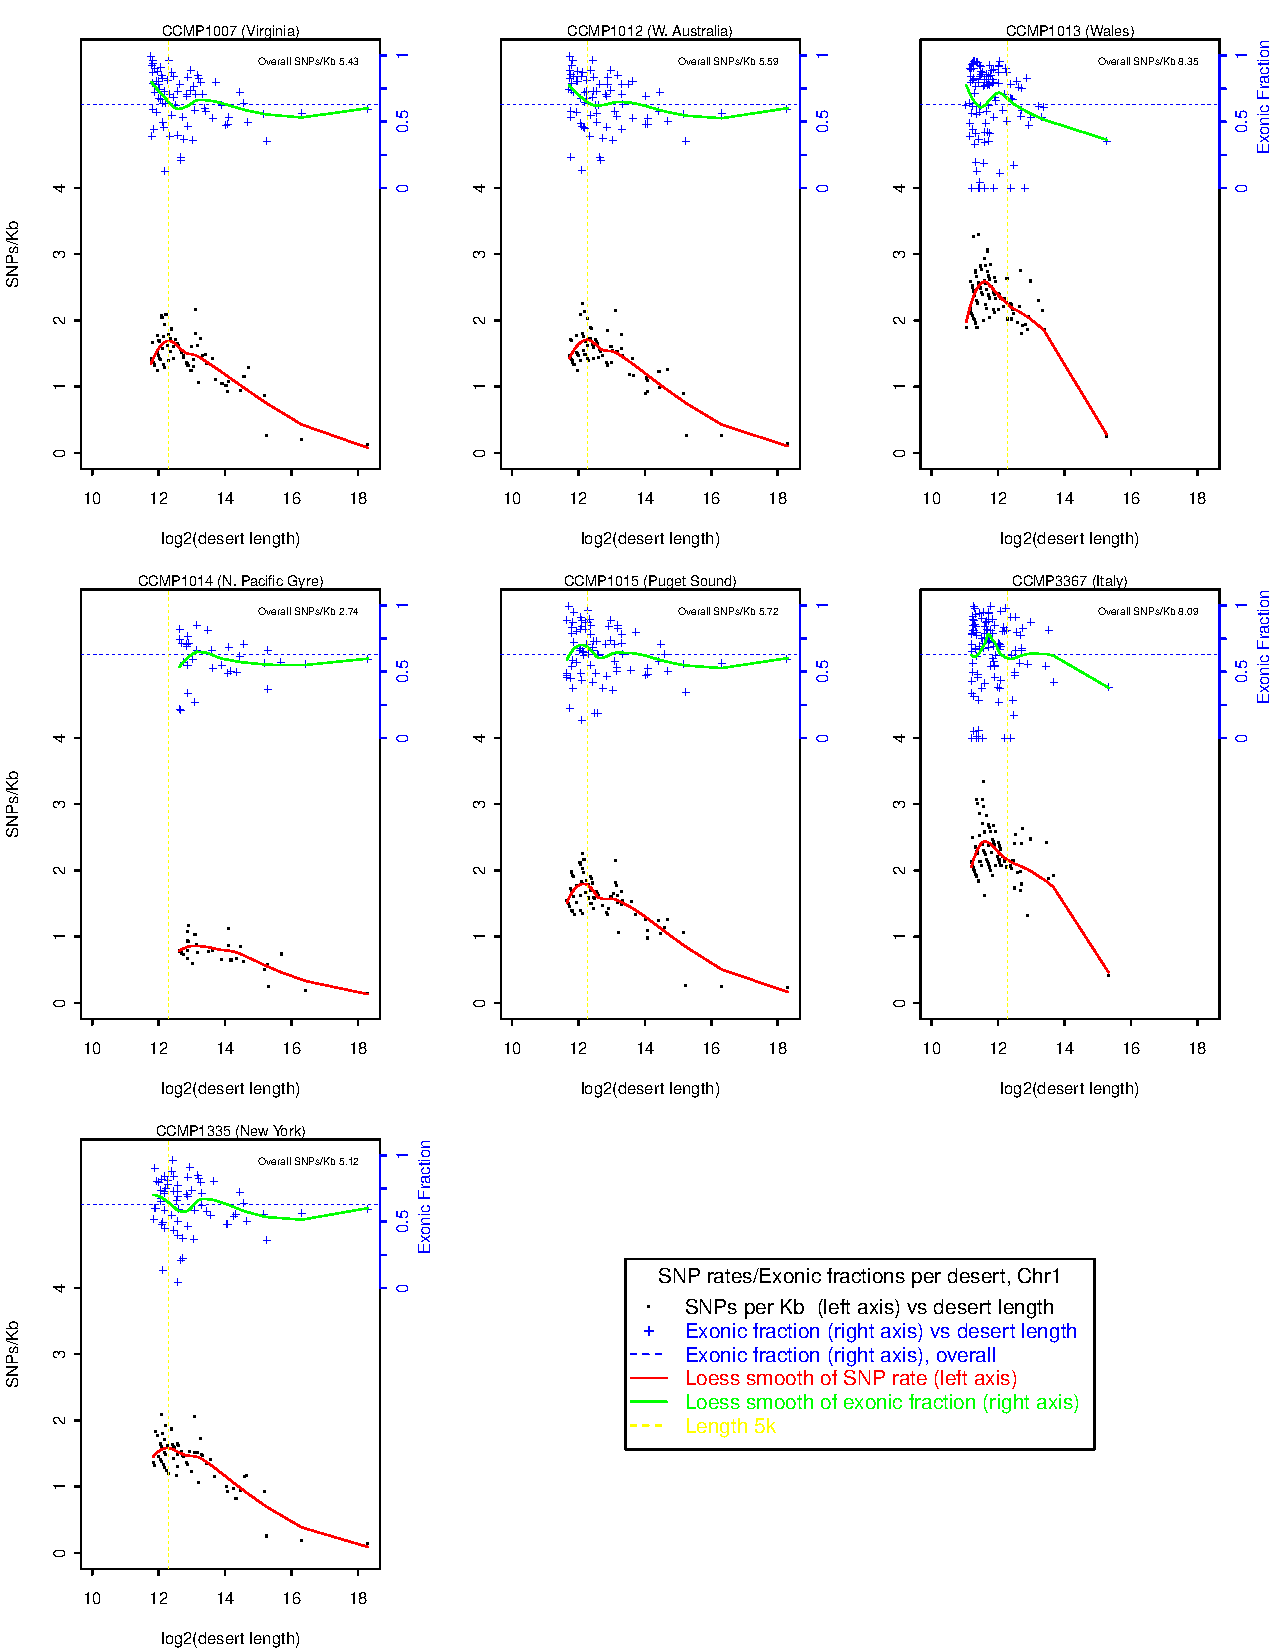
\includegraphics[width=\maxwidth]{figs-knitr/snp-ex-vs-deslen-1} \caption[SNP rates and Exonic fractions per desert]{SNP rates and Exonic fractions per desert}\label{fig:snp-ex-vs-deslen}
\end{figure}


\end{knitrout}

I.e., $\approx$30\% of Chr1 is desert in L-clade, which is about double the fraction in H-clade, and exons are not enriched in
deserts (in fact, they are marginally under represented).  SNPs are 1.29-1.51 times more common in non-exonic regions
than in exons.  (It is no surprise that purifying selection is stronger in exons, of course.)  SNPs are 3.91-8.44 times
more common in non-deserts compared to deserts.  (Again, unsurprising given how we defined deserts.)

Turning to Fig.~\ref{fig:snp-ex-vs-deslen}, we see that in-desert SNP rates tend to decline with increasing desert
length.  I don't have an explanation for this; ideas welcome.

Exonic fraction versus desert length is quite variable for shorter deserts, but shows some tendency to stabilize near
the global mean as length increases.  This presumably is a ``regression to the mean'' effect since longer deserts
average over more data.  (The largest desert in Italy/Wales is the obvious exception.)  The other trend that I think is
interesting is that most of the plots seem to show average exon content \emph{above} the global average for the shortest
deserts ($< 8$Kb, say).  There's not a lot of data and it's noisy, so this is debatable, but to me, at the scale of
gene-sized regions, this suggests some conflation of low SNP rates due to purifying selection vs low SNP rates due to
recent LoH; see additional discussion in sections~\ref{sec:small-deserts},\ref{sec:sim}

Out of curiousity, Fig~\ref{fig:snp-ex-deslen-pairs} is a pairs plot of \texttt{desert.data} for 1335.  
SNP rate vs exon fraction is the new info.  I find it mildly surprising that there is not an obvious 
correlation between them, but there does not appear to be (correlation is 
0.0741873).


\begin{knitrout}\footnotesize
\definecolor{shadecolor}{rgb}{0.969, 0.969, 0.969}\color{fgcolor}\begin{kframe}
\begin{alltt}
\hlstd{dd1ny} \hlkwb{<-} \hlstd{ddb.chr1}\hlopt{$}\hlstd{desert.data[[}\hlnum{1}\hlstd{]]}
\hlkwd{colnames}\hlstd{(dd1ny)[}\hlnum{1}\hlstd{]} \hlkwb{<-} \hlstr{'log2(desert.length)'}
\hlkwd{pairs}\hlstd{(dd1ny)}
\end{alltt}
\end{kframe}\begin{figure}
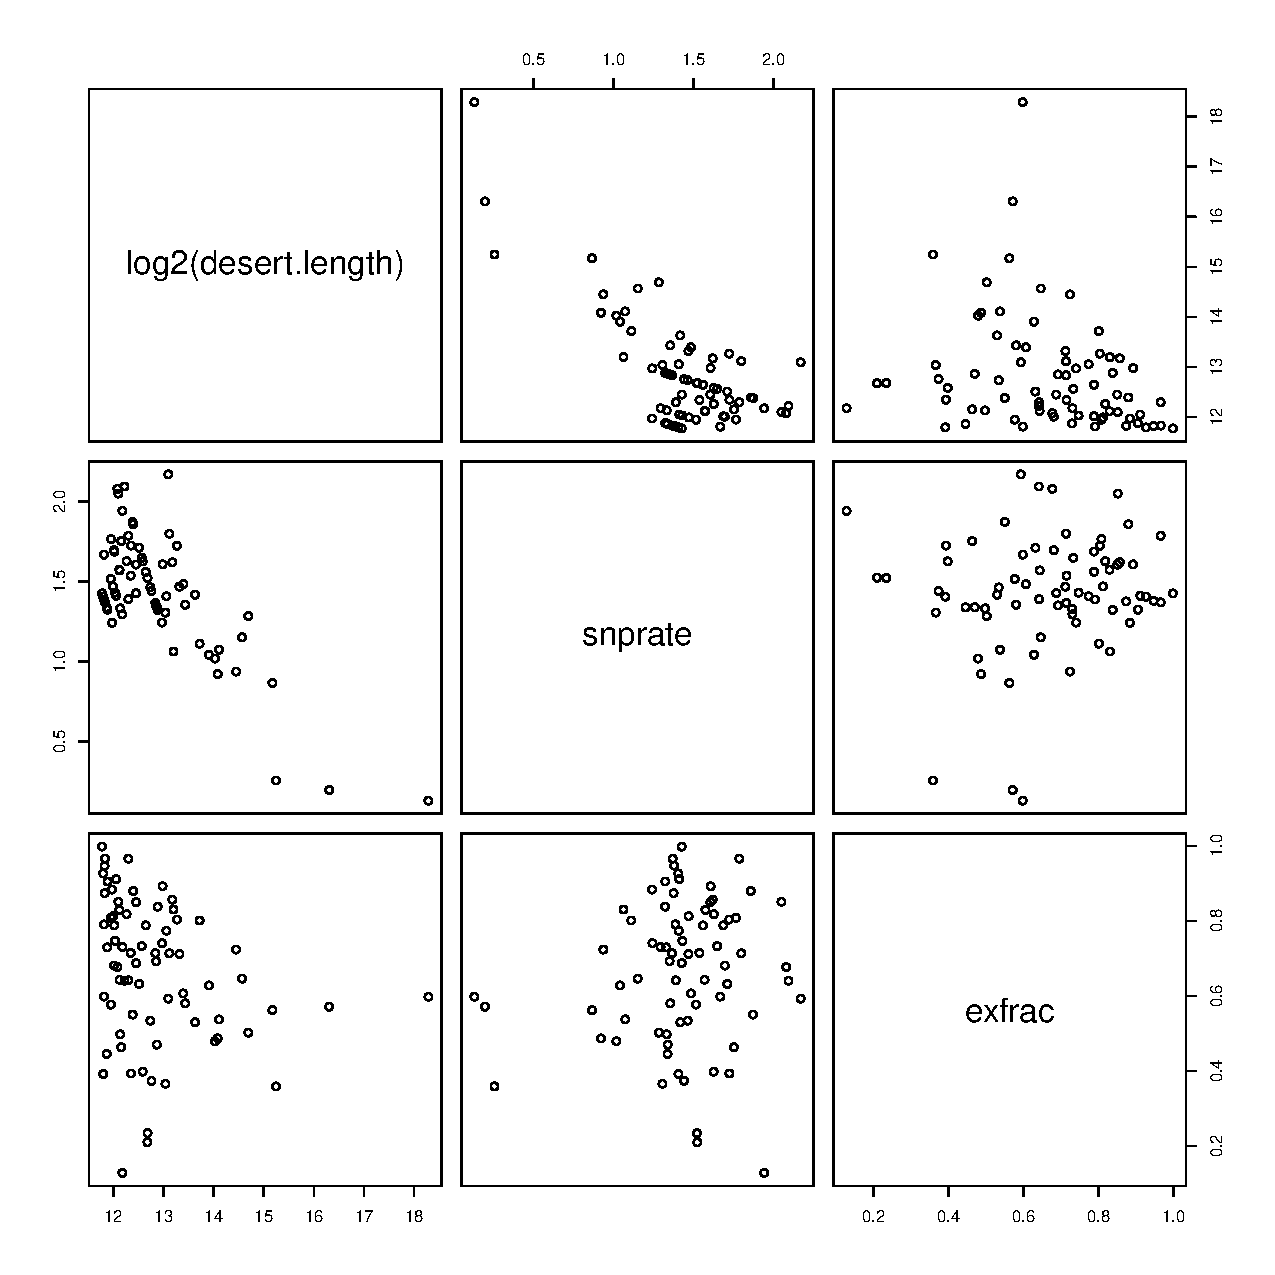
\includegraphics[width=\maxwidth]{figs-knitr/snp-ex-deslen-pairs-1} \caption[Pairs plot]{Pairs plot: 1335 SNP rates, Exonic fractions, log2(desert length), Chr1}\label{fig:snp-ex-deslen-pairs}
\end{figure}


\end{knitrout}

Redo all for full genome

\begin{knitrout}\footnotesize
\definecolor{shadecolor}{rgb}{0.969, 0.969, 0.969}\color{fgcolor}\begin{kframe}
\begin{alltt}
\hlkwa{if}\hlstd{(}\hlopt{!}\hlkwd{is.null}\hlstd{(snp.tables.full))\{}
  \hlstd{ddb.full} \hlkwb{<-} \hlkwd{des.dens.calc}\hlstd{(}\hlkwc{chr1.only} \hlstd{=} \hlnum{FALSE}\hlstd{,} \hlkwc{cnv.deletions} \hlstd{= cnv.dels.08.full,}
                            \hlkwc{snp.tables} \hlstd{= snp.tables.full)}
  \hlkwd{des.dens.plot}\hlstd{(ddb.full)}
\hlstd{\}}
\end{alltt}
\begin{verbatim}
#                        all_exon_% d_exon_% nd_exon_% des_% tot_snps nonex_snps/Kb exon_snps/Kb
# 1007 (Virginia)              57.8     59.2      57.1  34.2   165913          6.00         4.43
# 1012 (W. Australia)          57.8     59.3      57.1  34.8   171066          6.22         4.54
# 1013 (Wales)                 57.8     60.2      57.3  17.8   254581          9.44         6.62
# 1014 (N. Pacific Gyre)       57.8     58.2      57.7  29.0    91929          3.26         2.50
# 1015 (Puget Sound)           57.8     59.3      57.1  34.5   180440          6.60         4.75
# 3367 (Italy)                 57.8     60.9      57.0  20.8   246773          9.13         6.43
# 1335 (New York)              57.8     59.0      57.3  33.4   158343          5.62         4.30
#                        ne:e_snp_ratio nd_snps/Kb d_snps/Kb nd:d_snp_ratio d5_exon_% d5_snp/Kb
# 1007 (Virginia)                  1.36       7.24     0.940           7.70      58.5     0.860
# 1012 (W. Australia)              1.37       7.53     0.952           7.91      58.4     0.859
# 1013 (Wales)                     1.43       9.05     2.076           4.36      54.0     1.725
# 1014 (N. Pacific Gyre)           1.30       3.75     0.538           6.97      58.2     0.538
# 1015 (Puget Sound)               1.39       7.92     1.010           7.84      58.5     0.890
# 3367 (Italy)                     1.42       9.02     2.037           4.43      56.3     1.757
# 1335 (New York)                  1.31       6.87     0.835           8.22      58.3     0.762
#                         des.len des.len.uncnv
# 1007 (Virginia)        11147423      10178791
# 1012 (W. Australia)    11333481      10178803
# 1013 (Wales)            5802997       5033840
# 1014 (N. Pacific Gyre)  9464685       8509200
# 1015 (Puget Sound)     11252383      10356356
# 3367 (Italy)            6781702       6429335
# 1335 (New York)        10884516       9361571
\end{verbatim}
\end{kframe}\begin{figure}
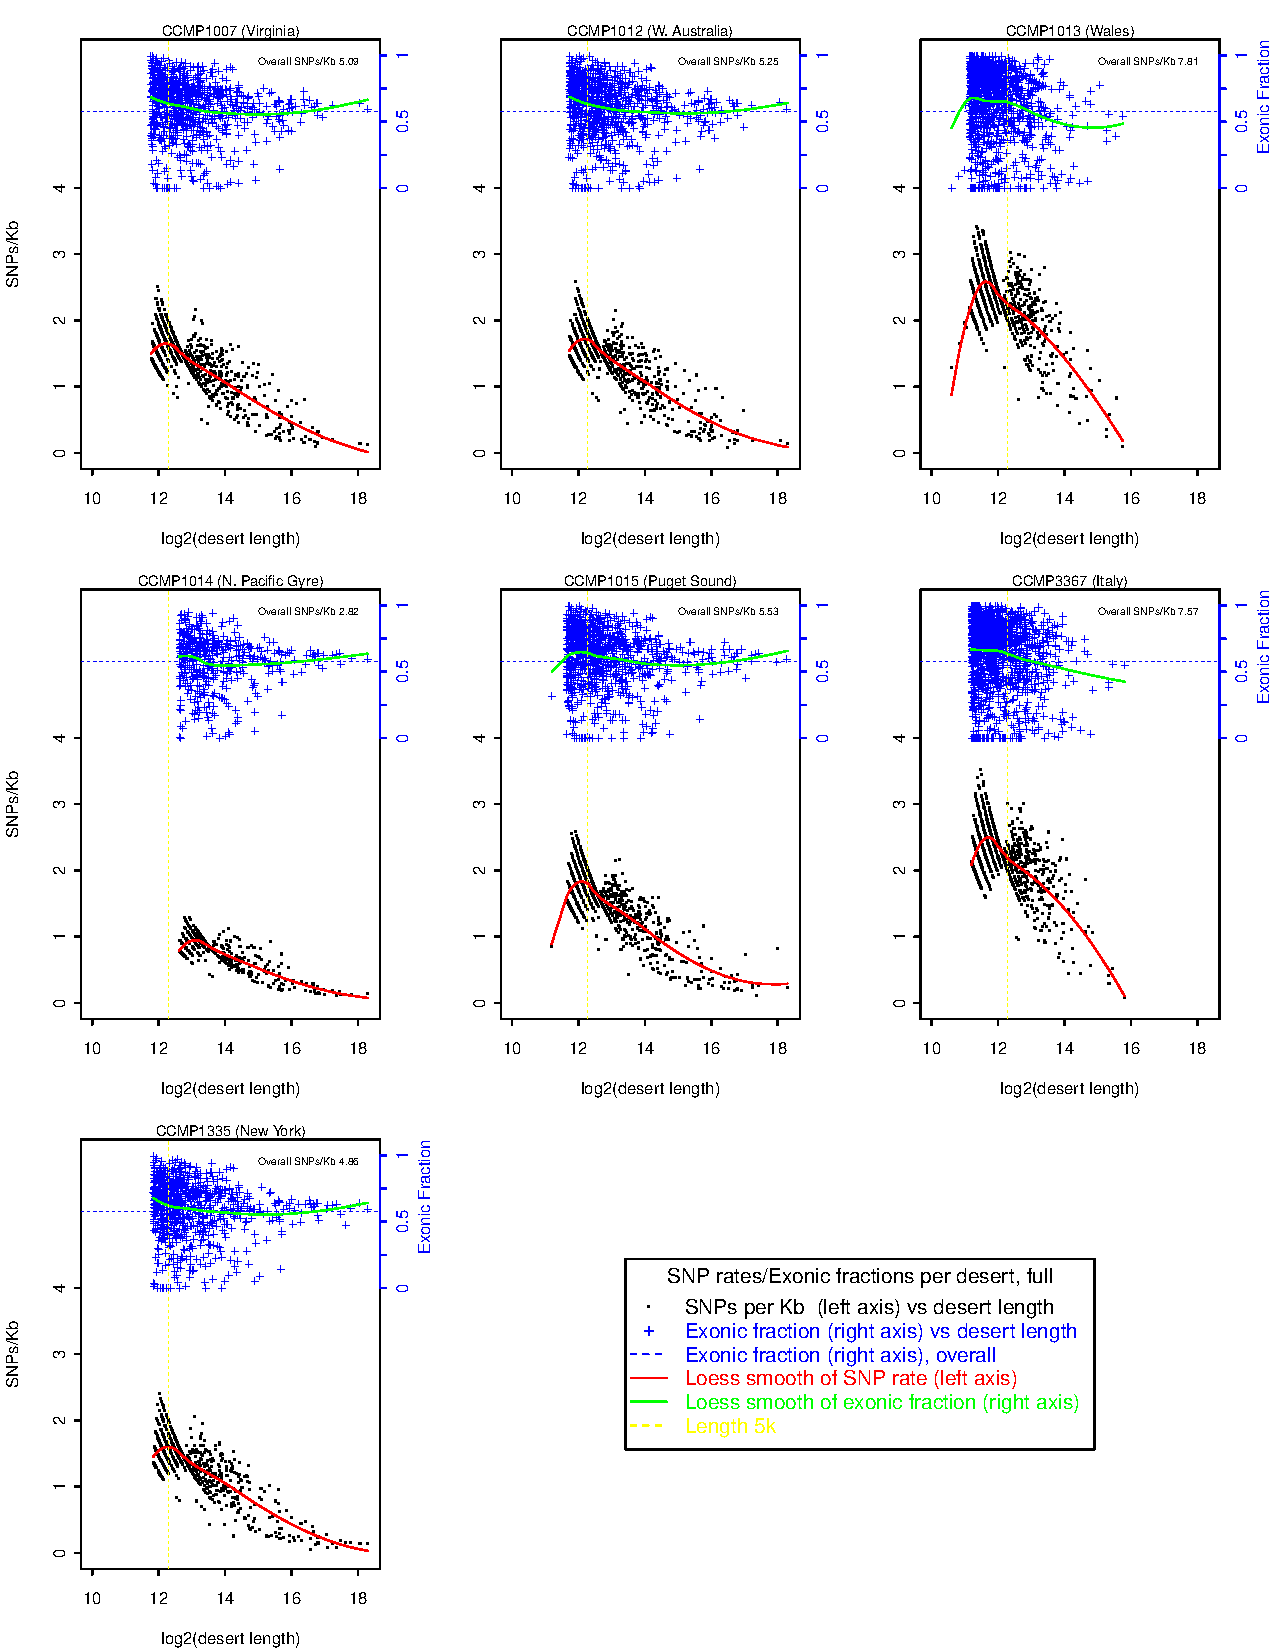
\includegraphics[width=\maxwidth]{figs-knitr/snp-ex-vs-deslen-full-1} \caption[SNP rates and Exonic fractions per desert]{SNP rates and Exonic fractions per desert}\label{fig:snp-ex-vs-deslen-full}
\end{figure}


\end{knitrout}

\begin{knitrout}\footnotesize
\definecolor{shadecolor}{rgb}{0.969, 0.969, 0.969}\color{fgcolor}\begin{kframe}
\begin{alltt}
\hlstd{ddfullny} \hlkwb{<-} \hlstd{ddb.full}\hlopt{$}\hlstd{desert.data[[}\hlnum{1}\hlstd{]]}
\hlkwd{colnames}\hlstd{(ddfullny)[}\hlnum{1}\hlstd{]} \hlkwb{<-} \hlstr{'log2(desert.length)'}
\hlkwd{pairs}\hlstd{(ddfullny,} \hlkwc{pch}\hlstd{=}\hlstr{'.'}\hlstd{)}
\end{alltt}
\end{kframe}\begin{figure}
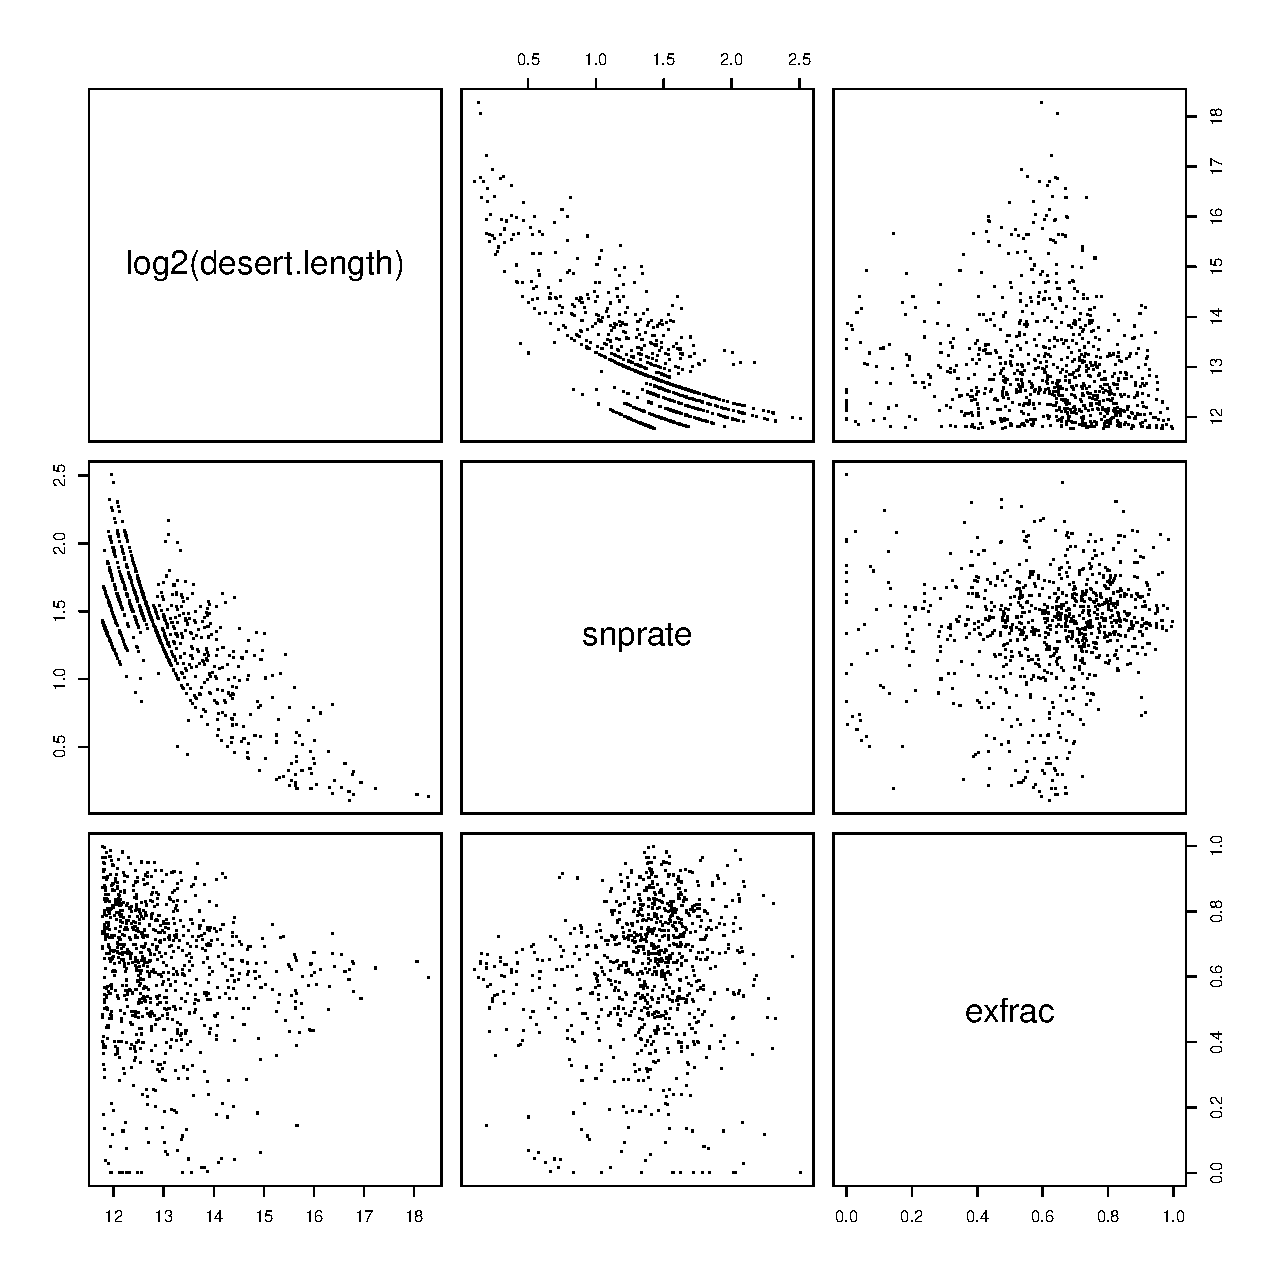
\includegraphics[width=\maxwidth]{figs-knitr/snp-ex-deslen-pairs-full-1} \caption[Pairs plot]{Pairs plot: 1335 SNP rates, Exonic fractions, log2(desert length), All Chrs}\label{fig:snp-ex-deslen-pairs-full}
\end{figure}


\end{knitrout}
\section{SNP Rate Plots, Coding \& Noncoding}

Key script is \texttt{snp.rates}, which depends on \texttt{shared.snp.calls} (both in \texttt{wlr.R}).

\noindent Parameters to snp.rate are:

{\footnotesize\begin{verbatim}
#  * snp.tables [default full.tables.01.26.14] - where to get SNP and other data; may be a subset
#    of the full data, but should include at least all of Chr1.
#
#  * nc [default FALSE] - If T, only count SNP rates within NonCoding DNA, or more accurately,
#    non-exonic DNA, as defined by the $exon flag in snp.tables
#
#  * length.thresh [default 5000] - only take deserts this long (see next).  
#
#  * length.thresh.eff [default F] - if T, length.thresh is based on ``effective desert length,''
#    i.e., number of desert positions that are not NA in genome, not in CNVnator deletion calls
#    if cnv.dels parameter supplied, and not exonic nc==T, else based on total length.
#
#  * cnv.dels [defualt NULL] - if supplied, table of CNVnator calls for effective length calc.
#
#  * merge.thresh - if non-null, an int specifying that the plot should include an overlay
#    reflecting merger of deserts within this distance of each other (absolute, not effective 
#    distance)
#
#  * strain [default 7] - which snps/deserts to use
#
#  * xCoordsReal [default F] - in plot, should markers be plotted at real chromosomal coords (T),
#    or at desert index (F)?
#
#  * xlab, ylab, main, legend,... [NULL] - plot axis labels, legend and title; if NULL, they are
#    calculated below; non-NULL values override the default calculation
#
#  * ... extra params assumed to be graphic params to main plot, e.g. cex.lab
\end{verbatim}}

% The following essentially reproduces Fig 3(a) from Tony's 7/15/2014 draft:

\begin{knitrout}\footnotesize
\definecolor{shadecolor}{rgb}{0.969, 0.969, 0.969}\color{fgcolor}\begin{kframe}
\begin{alltt}
\hlstd{sz} \hlkwb{<-} \hlstr{'scriptsize'} \hlstd{; fw} \hlkwb{<-} \hlnum{6.5} \hlstd{; fh} \hlkwb{<-} \hlnum{5} \hlstd{; fa} \hlkwb{<-} \hlstr{'center'} \hlcom{# knitr params: size, fig.\{width,height,align\}}
\hlkwd{print}\hlstd{(}\hlkwd{getOption}\hlstd{(}\hlstr{'width'}\hlstd{))}
\end{alltt}
\begin{verbatim}
# [1] 98
\end{verbatim}
\end{kframe}
\end{knitrout}
\iffalse
< < fourway-coding-5k-2k-o,size=sz,fig.width=fw,fig.height=fh,fig.align=fa > > =
snp.rates.o(length.thresh=5000,merge.thresh=2000,snpCalls=c(1,2,5,7),nc=F,ncmin=F,snp.tables=snp.tables.chr1)
@
< < fourway-coding-5k-2k,size=sz,fig.width=fw,fig.height=fh,fig.align=fa > > =
snp.rates(length.thresh=5000,merge.thresh=2000,snpCalls=c(1,2,5,7),nc=F,ncmin=F,snp.tables=snp.tables.chr1)
@

This one shows the effect of shifting to noncoding SNPs:

< < fourway-nc-5k-2k-o,size=sz,fig.width=fw,fig.height=fh,fig.align=fa > > =
snp.rates.o(length.thresh=5000,merge.thresh=2000,snpCalls=c(1,2,5,7),nc=T,ncmin=F,snp.tables=snp.tables.chr1)
@


< < fourway-nc-5k-2k,size=sz,fig.width=fw,fig.height=fh,fig.align=fa > > =
snp.rates(length.thresh=5000,merge.thresh=2000,snpCalls=c(1,2,5,7),nc=T,ncmin=F,snp.tables=snp.tables.chr1)
@

I.e., it's basically the same, but a bit noisier since the SNPcounts are smaller.

This one restricts to deserts with 5k noncoding:

< < fourway-nc-5knc-2k-o,size=sz,fig.width=fw,fig.height=fh,fig.align=fa > > =
snp.rates.o(length.thresh=5000,merge.thresh=2000,snpCalls=c(1,2,5,7),nc=T,ncmin=T,snp.tables=snp.tables.chr1)
@

< < fourway-nc-5knc-2k,size=sz,fig.width=fw,fig.height=fh,fig.align=fa > > =
snp.rates(length.thresh=5000,merge.thresh=2000,snpCalls=c(1,2,5,7),nc=T,ncmin=T,snp.tables=snp.tables.chr1)
@

I.e., noise in the deserts is lowered, but there are fewer of them.  The following reduces the length threshold to pull
in a few more deserts:

< < fourway-nc-3knc-2k-o,size=sz,fig.width=fw,fig.height=fh,fig.align=fa > > =
snp.rates.o(length.thresh=3000,merge.thresh=2000,snpCalls=c(1,2,5,7),nc=T,ncmin=T,snp.tables=snp.tables.chr1)
@

< < fourway-nc-3knc-2k,size=sz,fig.width=fw,fig.height=fh,fig.align=fa > > =
snp.rates(length.thresh=3000,merge.thresh=2000,snpCalls=c(1,2,5,7),nc=T,ncmin=T,snp.tables=snp.tables.chr1)
@
\fi

Some old code, hidden above, looked at 4-way shared SNPs, but it got complex and same story is visible in single strains.  E.g., looking at 1335, Chr 1, deserts longer than 3k, all snps, we have a clear separation of snp rate between deserts and non-deserts, and desert rates are quite uniform (excluding the few largest).  That suggested a ``burst'' of desert creation, e.g. via inbreeding.  (Variability in rates was somewhat reduced by looking at only non-exonic positions; that code is broken at the moment, but the pics are clear enough without it.)

\begin{knitrout}\scriptsize
\definecolor{shadecolor}{rgb}{0.969, 0.969, 0.969}\color{fgcolor}\begin{kframe}
\begin{alltt}
\hlkwd{snp.rates}\hlstd{(}\hlkwc{length.thresh}\hlstd{=}\hlnum{3000}\hlstd{,} \hlkwc{strain}\hlstd{=}\hlnum{7}\hlstd{,} \hlkwc{nc}\hlstd{=F,} \hlkwc{length.thresh.eff}\hlstd{=F,}
          \hlkwc{snp.tables}\hlstd{=snp.tables.chr1,} \hlkwc{des.tables}\hlstd{=des,} \hlkwc{cnv.dels}\hlstd{=cnv.dels.08.chr1)}
\end{alltt}
\begin{verbatim}
# snp.rates:
#                                   Type SNP.count Total.Positions    SNP.Rate
# 1                          total snps:     15582         3042585 0.005121303
# 2           after removing NAs in ref:     15581         3030824 0.005140846
# 3 after (also) removing CNVnator dels:     15573         3027004 0.005144691
\end{verbatim}
\end{kframe}

{\centering 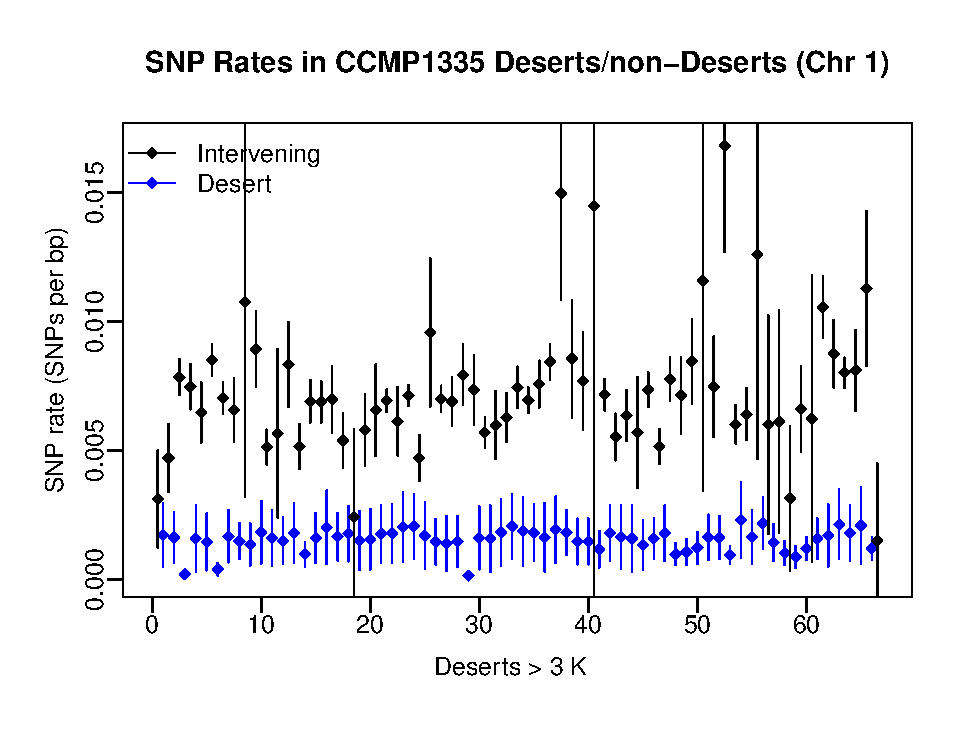
\includegraphics[width=\maxwidth]{figs-knitr/ny-coding-3k-o-1} 

}


\begin{kframe}\begin{verbatim}
# $desert.stats
#        Chr   Start     End  iStart    iEnd  sn          snr         snsig Length Len.eff
# 1     Chr1    3524    8144    3524    8144   8 0.0017312270 0.00061155112   4619    4621
# 2     Chr1   19185   25956   19185   25956  11 0.0016243355 0.00048935766   6770    6772
# 3     Chr1   91986  173031   91986  173031  16 0.0001976480 0.00004940711  81044   80952
# 4     Chr1  211997  215771  211997  215771   6 0.0015894040 0.00064835559   3773    3775
# 5     Chr1  234753  239556  234753  239556   7 0.0014571191 0.00055033785   4802    4804
# 6     Chr1  332426  371625  332426  371625  11 0.0003963964 0.00011949432  39198   27750
# 7     Chr1  448920  455478  448920  455478  11 0.0016770849 0.00050523593   6557    6559
# 8     Chr1  472361  484463  472361  484463  18 0.0014872346 0.00035028378  12101   12103
# 9     Chr1  485208  493330  485208  493330  11 0.0013541795 0.00040802393   8121    8123
# 10    Chr1  509678  514592  509678  514592   9 0.0018311292 0.00060981730   4913    4915
# 11    Chr1  559581  565191  559581  565191   9 0.0016039922 0.00053423508   5609    5611
# 12    Chr1  567310  574625  567310  574625  11 0.0015035539 0.00045299761   7314    7316
# 13    Chr1  586966  592480  586966  592480  10 0.0018132366 0.00057287568   5513    5515
# 14    Chr1  619261  636601  619261  636601  17 0.0009803356 0.00023764974  17339   17341
# 15    Chr1  676838  683680  676838  683680  11 0.0016074821 0.00048428438   6841    6843
# 16    Chr1  726771  730733  726771  730733   8 0.0020186727 0.00071298785   3961    3963
# 17    Chr1  747487  755335  747487  755335  13 0.0016562619 0.00045898384   7847    7849
# 18    Chr1  774815  781003  774815  781003  11 0.0017773469 0.00053541381   6187    6189
# 19    Chr1  781830  786461  781830  786461   7 0.0015112263 0.00057075807   4630    4632
# 20    Chr1  798541  803040  798541  803040   7 0.0015555556 0.00058748727   4498    4500
# 21    Chr1  811263  816907  811263  816907  10 0.0017714792 0.00055969450   5643    5645
# 22    Chr1  967028  972630  967028  972630  10 0.0017847582 0.00056388621   5601    5603
# 23    Chr1  986481  990903  986481  990903   9 0.0020348180 0.00067758223   4421    4423
# 24    Chr1 1157061 1162398 1157061 1162398  11 0.0020606969 0.00062068298   5336    5338
# 25    Chr1 1185747 1189862 1185747 1189862   7 0.0017006803 0.00064224989   4114    4116
# 26    Chr1 1194459 1201980 1194459 1201980  11 0.0014623770 0.00044060075   7520    7522
# 27    Chr1 1311718 1316715 1311718 1316715   7 0.0014005602 0.00052899118   4996    4998
# 28    Chr1 1347283 1353406 1347283 1353406   9 0.0014696277 0.00048951580   6122    6124
# 29    Chr1 1376223 1696217 1376223 1696217  45 0.0001406808 0.00002096999 319993  319873
# 30    Chr1 1712242 1716590 1712242 1716590   7 0.0016095654 0.00060786875   4347    4349
# 31    Chr1 1781479 1785263 1781479 1785263   6 0.0015852048 0.00064664399   3783    3785
# 32    Chr1 1798970 1803342 1798970 1803342   8 0.0018294077 0.00064620141   4371    4373
# 33    Chr1 1831079 1836424 1831079 1836424  11 0.0020576132 0.00061975512   5344    5346
# 34    Chr1 1882576 1886834 1882576 1886834   8 0.0018783752 0.00066348191   4257    4259
# 35    Chr1 2002722 2008786 2002722 2008786  11 0.0018136851 0.00054635050   6063    6065
# 36    Chr1 2045599 2049276 2045599 2049276   6 0.0016313214 0.00066544072   3676    3678
# 37    Chr1 2120068 2124728 2120068 2124728   9 0.0019309161 0.00064301700   4659    4661
# 38    Chr1 2128201 2138059 2128201 2138059  18 0.0018257430 0.00042993873   9857    9859
# 39    Chr1 2144596 2152086 2144596 2152086  11 0.0014684288 0.00044242274   7489    7491
# 40    Chr1 2160534 2167995 2160534 2167995  11 0.0014741356 0.00044414089   7460    7462
# 41    Chr1 2168203 2177606 2168203 2177606  11 0.0011697150 0.00035247602   9402    9404
# 42    Chr1 2252938 2259042 2252938 2259042  11 0.0018018018 0.00054277404   6103    6105
# 43    Chr1 2286005 2290252 2286005 2290252   7 0.0016486105 0.00062260233   4246    4246
# 44    Chr1 2316619 2320388 2316619 2320388   6 0.0015915119 0.00064921479   3768    3770
# 45    Chr1 2325305 2331260 2325305 2331260   8 0.0013431833 0.00047456799   5954    5956
# 46    Chr1 2395702 2405765 2395702 2405765  16 0.0015898251 0.00039714021  10062   10064
# 47    Chr1 2450937 2457083 2450937 2457083  11 0.0017897820 0.00053915643   6145    6146
# 48    Chr1 2500611 2523027 2500611 2523027  22 0.0009813980 0.00020913207  22415   22417
# 49    Chr1 2535911 2552809 2535911 2552809  18 0.0010651518 0.00025092494  16897   16899
# 50    Chr1 2565340 2578396 2565340 2578396  16 0.0012253963 0.00030616133  13055   13057
# 51    Chr1 2579087 2587650 2579087 2587650  14 0.0016376184 0.00043731342   8562    8549
# 52    Chr1 2595411 2604662 2595411 2604662  15 0.0016212711 0.00041827091   9250    9252
# 53    Chr1 2608587 2645487 2608587 2645487  35 0.0009484838 0.00016024697  36899   36901
# 54    Chr1 2689232 2693545 2689232 2693545  10 0.0023180343 0.00073217673   4312    4314
# 55    Chr1 2718992 2725045 2718992 2725045  10 0.0016518005 0.00052191359   6052    6054
# 56    Chr1 2725839 2734552 2725839 2734552  19 0.0021803994 0.00049967228   8712    8714
# 57    Chr1 2735885 2747021 2735885 2747021  16 0.0014366526 0.00035890506  11135   11137
# 58    Chr1 2748329 2767848 2748329 2767848  20 0.0010248002 0.00022903484  19518   19516
# 59    Chr1 2769438 2789983 2769438 2789983  18 0.0008760829 0.00020640426  20544   20546
# 60    Chr1 2799516 2823821 2799516 2823821  29 0.0011931701 0.00022143391  24304   24305
# 61    Chr1 2824623 2834776 2824623 2834776  16 0.0015757337 0.00039362294  10152   10154
# 62    Chr1 2863955 2868657 2863955 2868657   8 0.0017010419 0.00060089740   4701    4703
# 63    Chr1 2888988 2893675 2888988 2893675  10 0.0021331058 0.00067382746   4686    4688
# 64    Chr1 2988042 2994149 2988042 2994149  11 0.0018035744 0.00054330752   6106    6099
# 65    Chr1 3007328 3011154 3007328 3011154   8 0.0020904102 0.00073829874   3825    3827
# 66    Chr1 3016117 3041918 3016117 3041918  31 0.0012014573 0.00021565842  25800   25802
# 67 Overall      NA      NA      NA      NA 833 0.0008697668            NA 969294  957728
# 
# $nondesert.stats
#     usnlen   usn        usnr       usnsig
# 1     3523    11 0.003122339 0.0009399497
# 2    11040    52 0.004710145 0.0006516395
# 3    64726   508 0.007848469 0.0003468503
# 4    38947   291 0.007471692 0.0004363590
# 5    18981   123 0.006480164 0.0005824005
# 6    92869   791 0.008517374 0.0003015505
# 7    77285   544 0.007038882 0.0003007256
# 8    16882   111 0.006575050 0.0006220211
# 9      744     8 0.010752688 0.0037811551
# 10   16347   146 0.008931302 0.0007358516
# 11   44988   231 0.005134703 0.0003369702
# 12    2118    12 0.005665722 0.0016309133
# 13   12340   103 0.008346840 0.0008189990
# 14   26780   138 0.005153099 0.0004375293
# 15   40235   278 0.006909407 0.0004129646
# 16   43090   297 0.006892550 0.0003985656
# 17   16753   117 0.006983824 0.0006433962
# 18   19479   105 0.005390420 0.0005246314
# 19     826     2 0.002421308 0.0017100489
# 20   12076    70 0.005796621 0.0006908178
# 21    8222    54 0.006567745 0.0008908171
# 22  150102  1041 0.006935284 0.0002142040
# 23   13850    85 0.006137184 0.0006636253
# 24  166152  1186 0.007138042 0.0002065291
# 25   23348   110 0.004711324 0.0004481477
# 26    4596    44 0.009573542 0.0014363406
# 27  107237   751 0.007003180 0.0002546533
# 28   30567   211 0.006902869 0.0004735701
# 29   22816   181 0.007933029 0.0005873139
# 30   16024   118 0.007363954 0.0006754063
# 31   64881   370 0.005702748 0.0002956252
# 32   13706    82 0.005982781 0.0006587083
# 33   27736   174 0.006273435 0.0004740938
# 34   46151   344 0.007453793 0.0004003810
# 35  115887   806 0.006955051 0.0002441278
# 36   36812   279 0.007579050 0.0004520231
# 37   70790   598 0.008447521 0.0003439826
# 38    3472    52 0.014976959 0.0020613187
# 39    6536    56 0.008567931 0.0011400226
# 40    8447    65 0.007695040 0.0009507728
# 41     207     3 0.014492754 0.0083065406
# 42   75328   540 0.007168649 0.0003073818
# 43   26962   149 0.005526296 0.0004514791
# 44   26366   168 0.006371843 0.0004900296
# 45    4916    28 0.005695688 0.0010733140
# 46   64441   474 0.007355566 0.0003366075
# 47   45171   233 0.005158177 0.0003370507
# 48   43523   338 0.007766009 0.0004207718
# 49   12883    92 0.007141194 0.0007418578
# 50   12530   106 0.008459697 0.0008181954
# 51     690     8 0.011594203 0.0040753372
# 52    7760    58 0.007474227 0.0009777395
# 53    3924    66 0.016819572 0.0020528612
# 54   43733   263 0.006013765 0.0003697079
# 55   25446   163 0.006405722 0.0005001253
# 56     793    10 0.012610340 0.0039625166
# 57    1332     8 0.006006006 0.0021170575
# 58    1307     8 0.006120888 0.0021574274
# 59    1589     5 0.003146633 0.0014050014
# 60    9532    63 0.006609316 0.0008299392
# 61     801     5 0.006242197 0.0027828690
# 62   29178   308 0.010555898 0.0005982951
# 63   20330   178 0.008755534 0.0006533757
# 64   94366   757 0.008021957 0.0002903912
# 65   13178   107 0.008119593 0.0007817575
# 66    4962    56 0.011285772 0.0014995904
# 67     667     1 0.001499250 0.0014981261
# 68 2069276 14740 0.007123264           NA
# 
# $merged.desert.stats
# NULL
\end{verbatim}
\end{kframe}
\end{knitrout}

Unfortunately, Italy looked about the same:

\begin{knitrout}\scriptsize
\definecolor{shadecolor}{rgb}{0.969, 0.969, 0.969}\color{fgcolor}\begin{kframe}
\begin{alltt}
\hlkwd{snp.rates}\hlstd{(}\hlkwc{length.thresh}\hlstd{=}\hlnum{3000}\hlstd{,} \hlkwc{strain}\hlstd{=}\hlnum{6}\hlstd{,} \hlkwc{nc}\hlstd{=F,} \hlkwc{length.thresh.eff}\hlstd{=F,}
          \hlkwc{snp.tables}\hlstd{=snp.tables.chr1,} \hlkwc{des.tables}\hlstd{=des,} \hlkwc{cnv.dels}\hlstd{=cnv.dels.08.chr1)}
\end{alltt}
\begin{verbatim}
# snp.rates:
#                                   Type SNP.count Total.Positions    SNP.Rate
# 1                          total snps:     24613         3042585 0.008089503
# 2           after removing NAs in ref:     24611         3030824 0.008120234
# 3 after (also) removing CNVnator dels:     24286         2989495 0.008123780
\end{verbatim}
\end{kframe}

{\centering 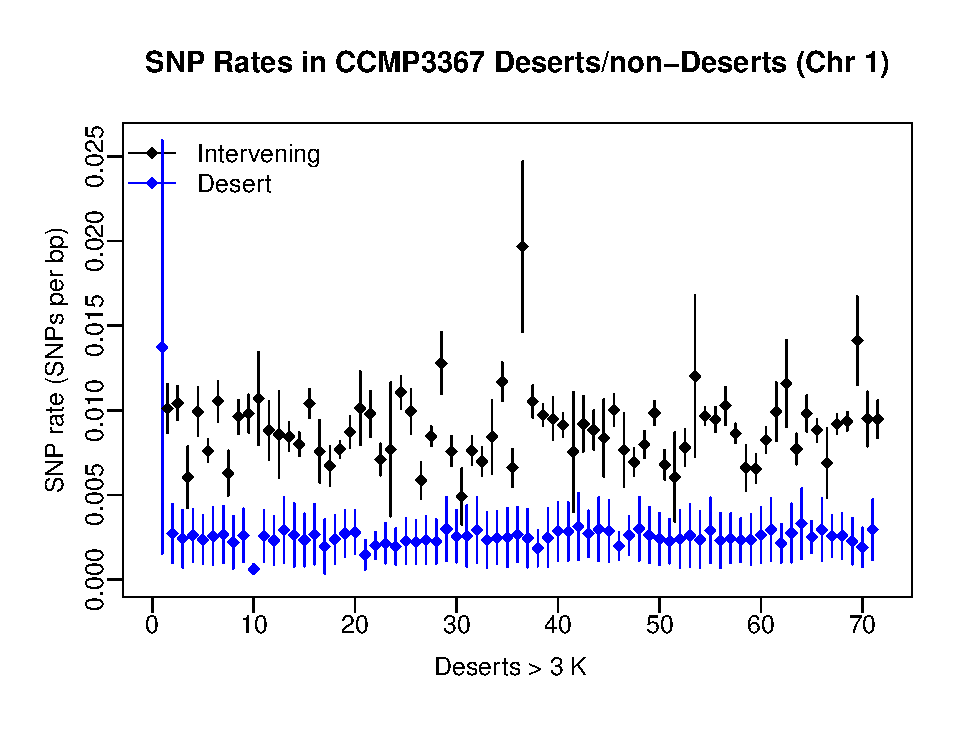
\includegraphics[width=\maxwidth]{figs-knitr/it-coding-3k-o-1} 

}


\begin{kframe}\begin{verbatim}
# $desert.stats
#        Chr   Start     End  iStart    iEnd  sn          snr        snsig Length Len.eff
# 1     Chr1   19835   25564   19835   25564   5 0.0137362637 0.0061007068   5728     364
# 2     Chr1   44985   48671   44985   48671  10 0.0027122322 0.0008565192   3685    3687
# 3     Chr1   95295   98615   95295   98615   8 0.0024089130 0.0008506529   3319    3321
# 4     Chr1  105899  110120  105899  110120  11 0.0026054003 0.0007845337   4220    4222
# 5     Chr1  129787  134460  129787  134460  11 0.0023534446 0.0007087548   4672    4674
# 6     Chr1  201747  205279  201747  205279   9 0.0025474101 0.0008480545   3531    3533
# 7     Chr1  234797  238555  234797  238555  10 0.0026602820 0.0008401353   3757    3759
# 8     Chr1  252883  256516  252883  256516   8 0.0022014309 0.0007774662   3632    3634
# 9     Chr1  295300  299518  295300  299518  11 0.0026072529 0.0007850909   4217    4219
# 10    Chr1  330737  371708  330737  371708  18 0.0006097354 0.0001436722  40970   29521
# 11    Chr1  377329  381622  377329  381622  11 0.0025617140 0.0007713959   4292    4294
# 12    Chr1  393545  397894  393545  397894  10 0.0022988506 0.0007261243   4348    4350
# 13    Chr1  403149  406240  403149  406240   9 0.0029107374 0.0009688327   3090    3092
# 14    Chr1  454162  457204  454162  457204   8 0.0026289846 0.0009282638   3041    3043
# 15    Chr1  523959  527820  523959  527820   9 0.0023303988 0.0007758939   3860    3862
# 16    Chr1  588264  591630  588264  591630   9 0.0026730027 0.0008898093   3365    3367
# 17    Chr1  600476  603550  600476  603550   6 0.0019512195 0.0007958045   3073    3075
# 18    Chr1  622760  627411  622760  627411  11 0.0023645744 0.0007121026   4650    4652
# 19    Chr1  749298  755191  749298  755191  16 0.0027146250 0.0006777345   5892    5894
# 20    Chr1  794428  801246  794428  801246  19 0.0027875587 0.0006386179   6817    6816
# 21    Chr1  809644  817209  809644  817209  11 0.0014538726 0.0004380403   7564    7566
# 22    Chr1  838470  851456  838470  851456  26 0.0020020020 0.0003922317  12985   12987
# 23    Chr1  883766  889853  883766  889853  13 0.0021353482 0.0005916064   6086    6088
# 24    Chr1  891807  898492  891807  898492  13 0.0019443614 0.0005387443   6684    6686
# 25    Chr1  946398  951244  946398  951244  11 0.0022694450 0.0006834865   4845    4847
# 26    Chr1  974301  979731  974301  979731  12 0.0022095378 0.0006371336   5429    5431
# 27    Chr1 1000419 1005118 1000419 1005118  11 0.0023404255 0.0007048386   4698    4700
# 28    Chr1 1108878 1114216 1108878 1114216  12 0.0022476119 0.0006481001   5337    5339
# 29    Chr1 1129473 1132822 1129473 1132822  10 0.0029850746 0.0009425535   3348    3350
# 30    Chr1 1171474 1175790 1171474 1175790  11 0.0025480658 0.0007672913   4315    4317
# 31    Chr1 1182917 1186040 1182917 1186040   8 0.0025608195 0.0009042264   3122    3124
# 32    Chr1 1231567 1234664 1231567 1234664   9 0.0029051001 0.0009669591   3096    3098
# 33    Chr1 1274867 1278288 1274867 1278288   8 0.0023378141 0.0008255754   3420    3422
# 34    Chr1 1285400 1289472 1285400 1289472  10 0.0024551927 0.0007754464   4071    4073
# 35    Chr1 1324902 1328139 1324902 1328139   8 0.0024706609 0.0008724308   3236    3238
# 36    Chr1 1349055 1353184 1349055 1353184  11 0.0026634383 0.0008019867   4128    4130
# 37    Chr1 1356236 1359515 1356236 1359515   8 0.0024390244 0.0008612731   3278    3280
# 38    Chr1 1406681 1413183 1406681 1413183  12 0.0018453022 0.0005322011   6501    6503
# 39    Chr1 1505488 1508725 1505488 1508725   8 0.0024706609 0.0008724308   3236    3238
# 40    Chr1 1532427 1536290 1532427 1536290  11 0.0028467909 0.0008571171   3862    3864
# 41    Chr1 1614730 1618602 1614730 1618602  11 0.0028401756 0.0008551282   3871    3873
# 42    Chr1 1620991 1624177 1620991 1624177  10 0.0031377471 0.0009906848   3185    3187
# 43    Chr1 1637999 1643902 1637999 1643902  16 0.0027100271 0.0006765881   5902    5904
# 44    Chr1 1670173 1673538 1670173 1673538  10 0.0029708853 0.0009380799   3364    3366
# 45    Chr1 1679883 1683370 1679883 1683370  10 0.0028669725 0.0009053157   3486    3488
# 46    Chr1 1730540 1742292 1730540 1742292  23 0.0019569472 0.0004076522  11751   11753
# 47    Chr1 1748818 1756900 1748818 1756900  21 0.0025980453 0.0005662030   8081    8083
# 48    Chr1 1798619 1801962 1798619 1801962  10 0.0029904306 0.0009442422   3342    3344
# 49    Chr1 1852074 1855888 1852074 1855888  10 0.0026212320 0.0008278192   3813    3815
# 50    Chr1 1935664 1939834 1935664 1939834  10 0.0023975066 0.0007572488   4169    4171
# 51    Chr1 1975423 1980728 1975423 1980728  12 0.0022615907 0.0006521263   5304    5306
# 52    Chr1 1984203 1987547 1984203 1987547   8 0.0023916293 0.0008445569   3343    3345
# 53    Chr1 2015126 2018203 2015126 2018203   8 0.0025990903 0.0009177222   3076    3078
# 54    Chr1 2020287 2023696 2020287 2023696   8 0.0023460411 0.0008284772   3408    3410
# 55    Chr1 2174860 2177965 2174860 2177965   9 0.0028976175 0.0009644721   3104    3106
# 56    Chr1 2246833 2250330 2246833 2250330   8 0.0022870212 0.0008076589   3496    3498
# 57    Chr1 2283251 2287781 2283251 2287781  11 0.0024287922 0.0007314186   4529    4529
# 58    Chr1 2393409 2398995 2393409 2398995  13 0.0023268301 0.0006445953   5585    5587
# 59    Chr1 2413382 2417621 2413382 2417621  10 0.0023584906 0.0007449402   4238    4240
# 60    Chr1 2455160 2458969 2455160 2458969  10 0.0026253610 0.0008291215   3808    3809
# 61    Chr1 2520005 2523404 2520005 2523404  10 0.0029411765 0.0009287129   3398    3400
# 62    Chr1 2536422 2542958 2536422 2542958  14 0.0021416552 0.0005717682   6535    6537
# 63    Chr1 2555252 2558899 2555252 2558899  10 0.0027412281 0.0008656635   3646    3648
# 64    Chr1 2596416 2599454 2596416 2599454  10 0.0032905561 0.0010388518   3037    3039
# 65    Chr1 2633712 2644861 2633712 2644861  28 0.0025112108 0.0004739780  11148   11150
# 66    Chr1 2721861 2725260 2721861 2725260  10 0.0029411765 0.0009287129   3398    3400
# 67    Chr1 2731787 2738445 2731787 2738445  17 0.0025529359 0.0006183870   6657    6659
# 68    Chr1 2842837 2848645 2842837 2848645  15 0.0025822000 0.0006658598   5807    5809
# 69    Chr1 2975148 2980023 2975148 2980023  11 0.0022559475 0.0006794261   4874    4876
# 70    Chr1 2988240 2994005 2988240 2994005  11 0.0019107174 0.0005755523   5764    5757
# 71    Chr1 3008448 3012179 3008448 3012179  11 0.0029474812 0.0008873884   3730    3732
# 72 Overall      NA      NA      NA      NA 807 0.0022954895           NA 368249  351559
# 
# $nondesert.stats
#     usnlen   usn        usnr       usnsig
# 1        0     0         NaN          NaN
# 2    19420   196 0.010092688 0.0007172591
# 3    42120   439 0.010422602 0.0004948445
# 4     7283    44 0.006041466 0.0009080299
# 5    19666   195 0.009915590 0.0007065410
# 6    67174   511 0.007607110 0.0003352363
# 7    29517   311 0.010536301 0.0005943030
# 8    14323    90 0.006283600 0.0006602653
# 9    38783   373 0.009617616 0.0004955808
# 10   31218   306 0.009802037 0.0005575922
# 11    5610    60 0.010695187 0.0013733392
# 12   11922   105 0.008807247 0.0008557060
# 13    5254    45 0.008564903 0.0012713008
# 14   47921   404 0.008430542 0.0004176634
# 15   66754   534 0.007999521 0.0003447857
# 16   56043   583 0.010402726 0.0004285901
# 17    8845    67 0.007574901 0.0009219098
# 18   19209   129 0.006715602 0.0005892871
# 19  121885   937 0.007687574 0.0002501749
# 20   39236   342 0.008716485 0.0004692748
# 21    8397    85 0.010122663 0.0010923857
# 22   21245   208 0.009790539 0.0006755204
# 23   32307   229 0.007088247 0.0004667415
# 24    1953    15 0.007680492 0.0019754641
# 25   47901   530 0.011064487 0.0004779444
# 26   23056   229 0.009932339 0.0006530797
# 27   20687   121 0.005849084 0.0005301775
# 28  103756   878 0.008462161 0.0002843732
# 29   15256   195 0.012781856 0.0009094591
# 30   38651   293 0.007580658 0.0004411849
# 31    7126    35 0.004911591 0.0008281691
# 32   43626   332 0.007610141 0.0004160685
# 33   40202   280 0.006964828 0.0004147761
# 34    7111    60 0.008437632 0.0010846883
# 35   35429   414 0.011685343 0.0005709379
# 36   20915   138 0.006598135 0.0005598145
# 37    3051    60 0.019665683 0.0025137410
# 38   47165   496 0.010516273 0.0004697052
# 39   92189   895 0.009708317 0.0003229342
# 40   23701   225 0.009493270 0.0006298735
# 41   78439   715 0.009115364 0.0003393380
# 42    2388    18 0.007537688 0.0017699416
# 43   13821   127 0.009188915 0.0008116295
# 44   26268   232 0.008832039 0.0005772855
# 45    6344    53 0.008354351 0.0011427547
# 46   47168   473 0.010027985 0.0004587695
# 47    6525    50 0.007662835 0.0010795285
# 48   41711   289 0.006928628 0.0004061520
# 49   50111   399 0.007962324 0.0003970246
# 50   79775   785 0.009840175 0.0003494787
# 51   35588   241 0.006771946 0.0004347398
# 52    3474    21 0.006044905 0.0013151134
# 53   27578   215 0.007796069 0.0005296109
# 54    2083    25 0.012001920 0.0023859360
# 55  151162  1459 0.009651897 0.0002514658
# 56   68864   651 0.009453415 0.0003687531
# 57   32920   338 0.010267315 0.0005555939
# 58  105627   912 0.008634156 0.0002846685
# 59   14386    95 0.006603642 0.0006752787
# 60   37538   246 0.006553359 0.0004164556
# 61   61031   503 0.008241713 0.0003659624
# 62   13017   129 0.009910118 0.0008682030
# 63    6993    81 0.011583012 0.0012795259
# 64   37501   289 0.007706461 0.0004515711
# 65   34257   336 0.009808214 0.0005324514
# 66   76988   679 0.008819556 0.0003369677
# 67    6526    45 0.006895495 0.0010243696
# 68  104383   960 0.009196900 0.0002954606
# 69  126502  1183 0.009351631 0.0002706168
# 70    8216   116 0.014118793 0.0013016099
# 71   14442   137 0.009486221 0.0008066093
# 72   30403   288 0.009472749 0.0005555370
# 73 2637936 23479 0.008900519           NA
# 
# $merged.desert.stats
# NULL
\end{verbatim}
\end{kframe}
\end{knitrout}

The reason, I think, for uniform desert rates is an artifact of desert selection: most deserts are a few K long, with 5-10 SNPs; with such a short length, the number of SNPs can't vary a lot, especially can't get a lot larger without ceasing to be a desert.

Now, go genome-wide and look at largest deserts.

\iffalse
< < ny-nc-3knc-2k-o,size=sz,fig.width=fw,fig.height=fh,fig.align=fa > > =
snp.rates.o(length.thresh=3000,merge.thresh=2000,snpCalls=7,nc=T,ncmin=T,snp.tables=snp.tables.chr1)
@

< < ny-nc-3knc-2k,size=sz,fig.width=fw,fig.height=fh,fig.align=fa > > =
snp.rates(length.thresh=3000,merge.thresh=2000,snpCalls=7,nc=T,ncmin=T,snp.tables=snp.tables.chr1)
@

I.e., still looking pretty good.  Finally, try it with no merging, just to reduce clutter:

< < ny-nc-3knc-nomerge-o,size=sz,fig.width=fw,fig.height=fh,fig.align=fa > > =
xx<-snp.rates.o(length.thresh=3000,merge.thresh=NULL,snpCalls=7,nc=T,ncmin=T,snp.tables=snp.tables.chr1)
@

< < ny-nc-3knc-nomerge,size=sz,fig.width=fw,fig.height=fh,fig.align=fa > > =
xx<-snp.rates(length.thresh=3000,merge.thresh=NULL,snpCalls=7,nc=T,ncmin=T,snp.tables=snp.tables.chr1)
@

< < it-nc-3knc-nomerge-o,size=sz,fig.width=fw,fig.height=fh,fig.align=fa > > =
snp.rates.o(length.thresh=3000,merge.thresh=NULL,snpCalls=6,nc=T,ncmin=T,snp.tables=snp.tables.chr1)
@

And once more, with some tweaks for the paper fig:

< < > > =
pdf('figs/ncsnps4paper.pdf',width=fw, height=fh)
xx<-snp.rates(length.thresh=3000,merge.thresh=NULL,snpCalls=7,nc=T,ncmin=T,
              snp.tables=snp.tables.chr1, 
              main='', 
              xlab='', #xlab='Chr1 Deserts, > 3K Non-exonic bp', 
              ylab='', #ylab='Non-exonic SNPS/bp', 
              cex.lab=1.3,
              cex.axis=1.2,
              mar=c(0,0,0,0),
              oma=c(5,150,0,0))
mtext('Chr1 Deserts, > 3K Non-exonic bp',side=1,line=2.8,cex=1.3)
mtext('Non-exonic SNPS/bp',side=2,line=2.8,cex=1.3)
dev.off()
@

\includegraphics{figs/ncsnps4paper.pdf}

Ditto, Italy:

< < > > =
pdf('figs/ncsnps4paperit.pdf',width=fw, height=fh)
xx<-snp.rates(length.thresh=3000,merge.thresh=NULL,snpCalls=6,nc=T,ncmin=T,
              snp.tables=snp.tables.chr1, 
              main='', 
              xlab='', #xlab='Chr1 Deserts, > 3K Non-exonic bp', 
              ylab='', #ylab='Non-exonic SNPS/bp', 
              cex.lab=1.3,
              cex.axis=1.2,
              mar=c(0,0,0,0),
              oma=c(5,150,0,0))
mtext('Chr1 Deserts, > 3K Non-exonic bp',side=1,line=2.8,cex=1.3)
mtext('Non-exonic SNPS/bp',side=2,line=2.8,cex=1.3)
dev.off()
@

\includegraphics{figs/ncsnps4paperit.pdf}

And an alternate idea: scale it to real chr 1 coords, to match panel a
< < > > =
pdf('figs/ncsnps4paperalt.pdf',width=fw, height=fh)
xx<-snp.rates(length.thresh=3000,merge.thresh=NULL,snpCalls=NULL,nc=T,ncmin=T,
              snp.tables=snp.tables.chr1, 
              xCoordsReal=TRUE,
              main='', 
              xlab='', #xlab='Chr1 Deserts, > 3K Non-exonic bp', 
              ylab='', #ylab='Non-exonic SNPS/bp', 
              cex.lab=1.3,
              cex.axis=1.2,
              mar=c(0,0,0,0),
              oma=c(5,150,0,0))
mtext('Chr1 Deserts, > 3K Non-exonic bp',side=1,line=2.8,cex=1.3)
mtext('Non-exonic SNPS/bp',side=2,line=2.8,cex=1.3)
dev.off()
@

\includegraphics{figs/ncsnps4paperalt.pdf}

\fi

\section{Big Deserts \& Fig 2B for paper}

A quick look at the $n=30$ deserts in each strain with largest effective size (``Len.eff'' in the tables generated below, which equals raw desert ``Length'' minus any overlap with ``NA'' regions in the reference sequence and/or hemi- or full-deletions called by CNVnator).  [The effective length correction usually has little effect, but for a few deserts it removes $>$50 K positions from consideration.  I am a little surprised it doesn't do more, since there are $\approx$225 K ``NA'' positions and around 1 M hemi-deletions (depending on TiC).   Either these tend create smaller deserts, or they aren't being called deserts.] 

\begin{knitrout}\footnotesize
\definecolor{shadecolor}{rgb}{0.969, 0.969, 0.969}\color{fgcolor}\begin{kframe}
\begin{alltt}
\hlkwa{if}\hlstd{(}\hlopt{!}\hlkwd{is.null}\hlstd{(snp.tables.full))\{}
  \hlstd{des.df.new} \hlkwb{<-} \hlstd{ddb.full}\hlopt{$}\hlstd{des.df.new} \hlcom{# desert tables as data frames}
  \hlstd{des.df.sorted} \hlkwb{<-} \hlkwd{vector}\hlstd{(}\hlstr{'list'}\hlstd{,}\hlnum{7}\hlstd{)} \hlcom{# sorted by length}
  \hlkwa{for}\hlstd{(st} \hlkwa{in} \hlnum{1}\hlopt{:}\hlnum{7}\hlstd{)\{}
    \hlstd{permute} \hlkwb{<-} \hlkwd{order}\hlstd{(des.df.new[[st]]}\hlopt{$}\hlstd{Length.uncnv,}\hlkwc{decreasing}\hlstd{=T)}
    \hlstd{des.df.sorted[[st]]} \hlkwb{<-} \hlstd{des.df.new[[st]][permute,}\hlkwd{c}\hlstd{(}\hlnum{1}\hlopt{:}\hlnum{3}\hlstd{,}\hlnum{5}\hlstd{,}\hlnum{6}\hlstd{,}\hlnum{4}\hlstd{,}\hlnum{7}\hlstd{)]}
    \hlkwd{names}\hlstd{(des.df.sorted[[st]])[}\hlnum{7}\hlstd{]} \hlkwb{<-} \hlstr{'Len.eff'} \hlcom{# shorten name}
  \hlstd{\}}

  \hlstd{keep.cols} \hlkwb{<-} \hlkwd{c}\hlstd{(}\hlnum{2}\hlstd{,}\hlnum{4}\hlstd{,}\hlnum{6}\hlstd{,}\hlnum{7}\hlstd{)}
  \hlstd{n} \hlkwb{<-} \hlnum{30}

  \hlcom{# n largest}
  \hlstd{bign} \hlkwb{<-} \hlkwa{NULL}
  \hlkwa{for}\hlstd{(st} \hlkwa{in} \hlkwd{c}\hlstd{(}\hlnum{1}\hlstd{,}\hlnum{2}\hlstd{,}\hlnum{4}\hlstd{,}\hlnum{5}\hlstd{,}\hlnum{7}\hlstd{,}\hlnum{3}\hlstd{,}\hlnum{6}\hlstd{))\{}
    \hlstd{perm} \hlkwb{<-} \hlkwd{order}\hlstd{(des.df.sorted[[st]]}\hlopt{$}\hlstd{iStart[}\hlnum{1}\hlopt{:}\hlstd{n])}
    \hlstd{one.strain.topn} \hlkwb{<-} \hlkwd{data.frame}\hlstd{(}\hlkwc{Chr}\hlstd{=}\hlkwd{as.character}\hlstd{(des.df.sorted[[st]]}\hlopt{$}\hlstd{Chr[}\hlnum{1}\hlopt{:}\hlstd{n][perm]),}
                                  \hlstd{des.df.sorted[[st]][}\hlnum{1}\hlopt{:}\hlstd{n, keep.cols][perm,],}
                                  \hlkwc{stringsAsFactors} \hlstd{=} \hlnum{FALSE}\hlstd{)}
    \hlstd{mins} \hlkwb{<-} \hlkwd{apply}\hlstd{(one.strain.topn[}\hlnum{1}\hlopt{:}\hlstd{n,}\hlkwd{c}\hlstd{(}\hlstr{'Length'}\hlstd{,}\hlstr{'Len.eff'}\hlstd{)],}\hlnum{2}\hlstd{,min)}
    \hlstd{maxs} \hlkwb{<-} \hlkwd{apply}\hlstd{(one.strain.topn[}\hlnum{1}\hlopt{:}\hlstd{n,}\hlkwd{c}\hlstd{(}\hlstr{'Length'}\hlstd{,}\hlstr{'Len.eff'}\hlstd{)],}\hlnum{2}\hlstd{,max)}
    \hlstd{one.strain.topn} \hlkwb{<-}
      \hlkwd{rbind}\hlstd{(one.strain.topn,}
            \hlkwd{data.frame}\hlstd{(}\hlkwc{Chr}\hlstd{=}\hlkwd{c}\hlstd{(}\hlstr{'Min:'}\hlstd{,}\hlstr{'Max:'}\hlstd{),}
                       \hlkwc{Start}\hlstd{=}\hlkwd{rep}\hlstd{(}\hlnum{NA}\hlstd{,}\hlnum{2}\hlstd{),}
                       \hlkwc{iStart}\hlstd{=}\hlkwd{rep}\hlstd{(}\hlnum{NA}\hlstd{,}\hlnum{2}\hlstd{),}
                       \hlkwc{Length}\hlstd{=}\hlkwd{c}\hlstd{(mins[}\hlnum{1}\hlstd{],maxs[}\hlnum{1}\hlstd{]),}
                       \hlkwc{Len.eff}\hlstd{=}\hlkwd{c}\hlstd{(mins[}\hlnum{2}\hlstd{],maxs[}\hlnum{2}\hlstd{])))}

    \hlkwa{if}\hlstd{(}\hlkwd{is.null}\hlstd{(bign))\{}
      \hlstd{bign} \hlkwb{<-} \hlstd{one.strain.topn}
    \hlstd{\}} \hlkwa{else} \hlstd{\{}
      \hlstd{bign} \hlkwb{<-} \hlkwd{cbind}\hlstd{(bign, one.strain.topn)}
    \hlstd{\}}
  \hlstd{\}}
  \hlkwd{rownames}\hlstd{(bign)} \hlkwb{<-} \hlkwa{NULL}
  \hlkwd{cat}\hlstd{(}\hlstr{'Largest 30 deserts per strain; ordered'}\hlstd{,} \hlkwd{substr}\hlstd{(}\hlkwd{st.locs}\hlstd{(}\hlnum{1}\hlopt{:}\hlnum{7}\hlstd{,}\hlkwc{loc}\hlstd{=F),} \hlnum{5}\hlstd{,}\hlnum{8}\hlstd{)[}\hlkwd{c}\hlstd{(}\hlnum{1}\hlstd{,}\hlnum{2}\hlstd{,}\hlnum{4}\hlstd{,}\hlnum{5}\hlstd{,}\hlnum{7}\hlstd{,}\hlnum{3}\hlstd{,}\hlnum{6}\hlstd{)],} \hlstr{'\textbackslash{}n'}\hlstd{)}
  \hlkwd{print}\hlstd{(bign)}
  \hlkwd{write.csv}\hlstd{(bign,}\hlstr{'bign.csv'}\hlstd{)}
  \hlcom{# lost due to CNV/NA:}
  \hlkwd{cbind}\hlstd{(} \hlkwc{d1007}\hlstd{=bign[,}\hlnum{4}\hlstd{]}\hlopt{-}\hlstd{bign[,}\hlnum{5}\hlstd{],}
         \hlkwc{d1012}\hlstd{=bign[,}\hlnum{9}\hlstd{]}\hlopt{-}\hlstd{bign[,}\hlnum{10}\hlstd{],}
         \hlkwc{d1014}\hlstd{=bign[,}\hlnum{14}\hlstd{]}\hlopt{-}\hlstd{bign[,}\hlnum{15}\hlstd{],}
         \hlkwc{d1015}\hlstd{=bign[,}\hlnum{19}\hlstd{]}\hlopt{-}\hlstd{bign[,}\hlnum{20}\hlstd{],}
         \hlkwc{d1335}\hlstd{=bign[,}\hlnum{24}\hlstd{]}\hlopt{-}\hlstd{bign[,}\hlnum{25}\hlstd{],}
         \hlkwc{d1013}\hlstd{=bign[,}\hlnum{29}\hlstd{]}\hlopt{-}\hlstd{bign[,}\hlnum{30}\hlstd{],}
         \hlkwc{d3367}\hlstd{=bign[,}\hlnum{34}\hlstd{]}\hlopt{-}\hlstd{bign[,}\hlnum{35}\hlstd{]}
  \hlstd{)}
\hlstd{\}}
\end{alltt}
\begin{verbatim}
# Largest 30 deserts per strain; ordered 1007 1012 1014 1015 1335 1013 3367 
#          Chr   Start   iStart Length Len.eff       Chr   Start   iStart Length Len.eff   Chr
# 1       Chr1   91986    91986  81045   80953      Chr1   91986    91986  81045   80968  Chr1
# 2       Chr1 1376212  1376212 320005  319894      Chr1 1376223  1376223 319994  319921  Chr1
# 3       Chr2 1058550  4101135  65971   65970      Chr2 1058550  4101135  65971   65971  Chr1
# 4       Chr2 1413816  4456401  66485   66485      Chr2 1413816  4456401  66485   66485  Chr2
# 5       Chr5       1 10592156  61354   61351      Chr5       1 10592156  62200   62123  Chr2
# 6       Chr5  798373 11390528 153878  153878      Chr5  798423 11390578 153828  147528  Chr2
# 7       Chr5 1703594 12295749  96270   96270      Chr5 1703594 12295749  96270   96270  Chr2
# 8       Chr5 2119647 12711802 107108  107102      Chr5 2119647 12711802 107108  107108  Chr5
# 9       Chr6  350440 13248567 111828  111820      Chr6  350440 13248567 111595  111585  Chr5
# 10      Chr8 1060806 18022847 106548  106534      Chr8 1060806 18022847 105965  105954  Chr5
# 11      Chr9  825287 19054526  87057   87057      Chr9  808017 19037256 104327  104327  Chr6
# 12      Chr9  995501 19224740  55619   55619      Chr9  995586 19224825  55534   55534  Chr6
# 13      Chr9 1059962 19289201  63104   63102      Chr9 1060017 19289256  62979   62979  Chr6
# 14     Chr10  510271 19930570  50922   50911    Chr11a   45832 20571799 128488  128462  Chr8
# 15    Chr11a   45832 20571799  65547   65540    Chr11a  226847 20752814  58511   58511  Chr9
# 16    Chr11a  111716 20637683  51247   51227    Chr11a  334100 20860067  66371   66353  Chr9
# 17    Chr11a  400836 20926803  60496   60494    Chr11a  400836 20926803  60860   60860 Chr10
# 18    Chr11a  547035 21073002  85177   85177    Chr11a  547050 21073017  60495   53995 Chr12
# 19     Chr12   87502 21502454  55051   55047    Chr11a  654830 21180797  72317   72317 Chr13
# 20     Chr13       1 22543335  53346   53333     Chr12   86515 21501467  57426   57426 Chr13
# 21     Chr13  125227 22668561 113461  113439     Chr13  125227 22668561 113678  113655 Chr13
# 22     Chr13  488706 23032040 100813  100785     Chr13  531852 23075186  57667   57660 Chr13
# 23     Chr13  698665 23241999  79709   79704     Chr13  698665 23241999  79617   79606 Chr17
# 24     Chr17  264204 26418797  51270   51265     Chr17  499780 26654373  62973   62963 Chr17
# 25     Chr17  499806 26654399  62947   62923     Chr17  564030 26718623  67345   67345 Chr17
# 26     Chr18  135703 26950220  50940   50840     Chr18  189799 27004316 113782  113775 Chr18
# 27     Chr18  189799 27004316 113782  113775 Chr19a_19  221515 27863085  56321   55121 Chr18
# 28 Chr19a_19  221676 27863246  56148   54948 Chr19b_31    4628 28253437  73745   73745 Chr22
# 29     Chr22       1 29491915 125776   73100 Chr19c_29   33384 28433870  82201   81601 Chr22
# 30     Chr22  798029 30289943  84939   84924     Chr22  798659 30290573 102812  102799 Chr22
# 31      Min:      NA       NA  50922   50840      Min:      NA       NA  55534   53995  Min:
# 32      Max:      NA       NA 320005  319894      Max:      NA       NA 319994  319921  Max:
#      Start   iStart Length Len.eff    Chr   Start   iStart Length Len.eff   Chr   Start   iStart
# 1    86447    86447  87666   87578   Chr1   91986    91986  81045   80947  Chr1   91986    91986
# 2  1375768  1375768 320634  320574   Chr1 1376223  1376223 319994  319913  Chr1 1376223  1376223
# 3  2734786  2734786  52797   52797   Chr2 1058550  4101135  65971   65971  Chr2 1058459  4101044
# 4  1055991  4098576  66547   66547   Chr2 1413975  4456560  66304   66304  Chr2 1413685  4456270
# 5  1413467  4456052  89481   89481   Chr2 2304492  5347077 176396  176364  Chr2 2239502  5282087
# 6  2240370  5282955  58129   58129   Chr5  798373 11390528 153878  153878  Chr2 2304333  5346918
# 7  2303718  5346303 178045  178020   Chr5 1703729 12295884  96135   96135  Chr5  798329 11390484
# 8   798283 11390438 155010  155010   Chr5 2119647 12711802 107108  107108  Chr5 1703538 12295693
# 9  1702551 12294706  97681   97681   Chr6  350440 13248567 111828  111818  Chr5 2119568 12711723
# 10 2119193 12711348 108513  108513   Chr8 1060806 18022847 105965  105954  Chr6  350354 13248481
# 11  350288 13248415 112333  112333   Chr9  825287 19054526  86587   86587  Chr7  693486 15663093
# 12 1514641 14412768  53420   53420   Chr9  995501 19224740  55409   55404  Chr8 1060717 18022758
# 13 1568670 14466797  60963   60958   Chr9 1061031 19290270  62141   62141  Chr9  808017 19037256
# 14 1060806 18022847 105983  105969  Chr10  510263 19930562  50930   50928  Chr9  995586 19224825
# 15  806621 19035860 106374  106369 Chr11a   42513 20568480 133483  131709  Chr9 1059962 19289201
# 16  994768 19224007 129602  129602 Chr11a  226885 20752852 258344  257328 Chr10  510493 19930792
# 17  510179 19930478  51035   51033 Chr11a  488445 21014412  55954   55954 Chr12   86223 21501175
# 18  946602 22361554  55089   51576 Chr11a  544609 21070576  87609   87609 Chr12  947336 22362288
# 19       1 22543335  53516   53516  Chr13       1 22543335  53346   53342 Chr13       1 22543335
# 20  124789 22668123 116100  116092  Chr13  125227 22668561 113678  113650 Chr13  125227 22668561
# 21  487469 23030803 102423  102403  Chr13  488706 23032040 100813  100787 Chr13  488706 23032040
# 22  697580 23240914  81087   81087  Chr13  698665 23241999  79617   79608 Chr13  698665 23241999
# 23  264204 26418797  51305   51305  Chr17  264400 26418993  51074   51071 Chr17  264204 26418797
# 24  499807 26654400  63208   63196  Chr17  499794 26654387  62974   62969 Chr17  499611 26654204
# 25  563839 26718432  68020   68020  Chr17  563866 26718459  67500   67499 Chr17  563803 26718396
# 26  134397 26948914  52676   52589  Chr18  136001 26950518  50642   50557 Chr18  135701 26950218
# 27  189799 27004316 115668  115668  Chr18  189835 27004352 113374  113354 Chr18  189825 27004342
# 28       1 29491915 127127   74454  Chr22       1 29491915 112025   59840 Chr22       1 29491915
# 29  156665 29648579  51065   51065  Chr22  157075 29648989  50655   50655 Chr22  157075 29648989
# 30  797849 30289763 103830  103825  Chr22  798291 30290205  84677   84669 Chr22  797909 30289823
# 31      NA       NA  51035   51033   Min:      NA       NA  50642   50557  Min:      NA       NA
# 32      NA       NA 320634  320574   Max:      NA       NA 319994  319913  Max:      NA       NA
#    Length Len.eff       Chr   Start   iStart Length Len.eff   Chr   Start   iStart Length Len.eff
# 1   81045   80960      Chr1  332712   332712  39367   27933  Chr1  330737   330737  40971   29577
# 2  319994  319943      Chr2  665676  3708261  12646   12646  Chr2 1515552  4558137  17026   17026
# 3   66062   66062      Chr2 2327989  5370574  19615   19600  Chr2 1600432  4643017  13991   13991
# 4   88350   88350      Chr2 2409780  5452365  12082   12082  Chr2 2164635  5207220  13765   13765
# 5   58997   58997      Chr2 2664737  5707322  18610   18610  Chr2 2329924  5372509  14675   14663
# 6  273340   99126      Chr4 1126400  9316232  12038   12038  Chr2 2408729  5451314  15858   15858
# 7  153922  153922      Chr4 2111249 10301081  11254   11245  Chr2 2661656  5704241  19852   19852
# 8   96326   96326      Chr5   31571 10623726  12411   12411  Chr3 1650177  7399957  14845   14845
# 9  107412  107412      Chr5 2072197 12664352  17103   17025  Chr4   20687  8210519  15840   15840
# 10 112226  112226      Chr5 2274803 12866958  14272   14272  Chr4   94053  8283885  15082   15082
# 11  50166   50166      Chr6 1372617 14270744  12613   12613  Chr4 1148253  9338085  14635   14635
# 12 135858  135843      Chr6 1759576 14657703  15140   15140  Chr5  393711 10985866  21374   21374
# 13 104379  104376      Chr6 2046236 14944363  18698   18683  Chr5 1504244 12096399  13884   13884
# 14  55678   55678      Chr7       1 14969608  12271   12129  Chr5 2072471 12664626  17826   17816
# 15  63278   63278      Chr8   14584 16976625  25735   25735  Chr5 2142394 12734549  19650   19650
# 16  50702   50702      Chr9  163296 18392535  14720   14720  Chr8   15586 16977627  25215   25215
# 17  49803   49803      Chr9 1003970 19233209  41669   41669  Chr9  570855 18800094  25223   25223
# 18  53955   50433     Chr12  641238 22056190  28549   28243  Chr9 1002413 19231652  44580   44580
# 19  53387   53385     Chr12  693433 22108385  12929   12929 Chr10  327254 19747553  14180   14180
# 20 113678  113671     Chr12  755960 22170912  13503   13503 Chr12   99678 21514630  15421   15421
# 21 100813  100804     Chr12  947935 22362887  48242   44720 Chr12  642125 22057077  26870   26556
# 22  79788   79785     Chr13  993368 23536702  14320   14320 Chr12  755258 22170210  15327   15327
# 23  51270   51270     Chr15  907874 25502047  19657   19657 Chr12  948542 22363494  16775   16775
# 24  63157   63151    Chr16b   80675 26065892  12800   12800 Chr12  966724 22381676  29339   25823
# 25  67572   67569     Chr17  590347 26744940  39605   39601 Chr14   34634 23630164  15916   15916
# 26  50942   50857     Chr18  541405 27355922  33899   33899 Chr17  589849 26744442  41419   41414
# 27 113906  113906 Chr19a_19  561315 28202885  14789   14789 Chr17  631536 26786129  19035   19035
# 28 114623   62482 Chr19a_19  585569 28227139  12404   11930 Chr18  542703 27357220  18013   18013
# 29  50835   50835     Chr22  501449 29993363  11179   11179 Chr22  662851 30154765  18887   18887
# 30 103567  103552     Chr22  685423 30177337  18411   14127 Chr22  685752 30177666  19725   15441
# 31  49803   49803      Min:      NA       NA  11179   11179  Min:      NA       NA  13765   13765
# 32 319994  319943      Max:      NA       NA  48242   44720  Max:      NA       NA  44580   44580
#       d1007 d1012 d1014 d1015  d1335 d1013 d3367
#  [1,]    92    77    88    98     85 11434 11394
#  [2,]   111    73    60    81     51     0     0
#  [3,]     1     0     0     0      0    15     0
#  [4,]     0     0     0     0      0     0     0
#  [5,]     3    77     0    32      0     0    12
#  [6,]     0  6300     0     0 174214     0     0
#  [7,]     0     0    25     0      0     9     0
#  [8,]     6     0     0     0      0     0     0
#  [9,]     8    10     0    10      0    78     0
# [10,]    14    11     0    11      0     0     0
# [11,]     0     0     0     0      0     0     0
# [12,]     0     0     0     5     15     0     0
# [13,]     2     0     5     0      3    15     0
# [14,]    11    26    14     2      0   142    10
# [15,]     7     0     5  1774      0     0     0
# [16,]    20    18     0  1016      0     0     0
# [17,]     2     0     2     0      0     0     0
# [18,]     0  6500  3513     0   3522   306     0
# [19,]     4     0     0     4      2     0     0
# [20,]    13     0     8    28      7     0     0
# [21,]    22    23    20    26      9  3522   314
# [22,]    28     7     0     9      3     0     0
# [23,]     5    11     0     3      0     0     0
# [24,]     5    10    12     5      6     0  3516
# [25,]    24     0     0     1      3     4     0
# [26,]   100     7    87    85     85     0     5
# [27,]     7  1200     0    20      0     0     0
# [28,]  1200     0 52673 52185  52141   474     0
# [29,] 52676   600     0     0      0     0     0
# [30,]    15    13     5     8     15  4284  4284
# [31,]    82  1539     2    85      0     0     0
# [32,]   111    73    60    81     51  3522     0
\end{verbatim}
\begin{alltt}
  \hlcom{# Some generic desert stats}
  \hlstd{dsum.df} \hlkwb{<-} \hlkwd{rbind}\hlstd{(}
    \hlkwd{summary}\hlstd{(des.df[[}\hlnum{1}\hlstd{]]}\hlopt{$}\hlstd{Length),}
    \hlkwd{summary}\hlstd{(des.df[[}\hlnum{2}\hlstd{]]}\hlopt{$}\hlstd{Length),}
    \hlkwd{summary}\hlstd{(des.df[[}\hlnum{3}\hlstd{]]}\hlopt{$}\hlstd{Length),}
    \hlkwd{summary}\hlstd{(des.df[[}\hlnum{4}\hlstd{]]}\hlopt{$}\hlstd{Length),}
    \hlkwd{summary}\hlstd{(des.df[[}\hlnum{5}\hlstd{]]}\hlopt{$}\hlstd{Length),}
    \hlkwd{summary}\hlstd{(des.df[[}\hlnum{6}\hlstd{]]}\hlopt{$}\hlstd{Length),}
    \hlkwd{summary}\hlstd{(des.df[[}\hlnum{7}\hlstd{]]}\hlopt{$}\hlstd{Length)}
  \hlstd{)}
  \hlkwd{row.names}\hlstd{(dsum.df)} \hlkwb{<-} \hlkwd{names}\hlstd{(des.df)}
  \hlstd{dsum.df} \hlkwb{<-} \hlkwd{cbind}\hlstd{(}\hlkwc{N}\hlstd{=}\hlkwd{unlist}\hlstd{(}\hlkwd{lapply}\hlstd{(des.df,nrow)),dsum.df)}
  \hlkwd{print}\hlstd{(dsum.df)}
\end{alltt}
\begin{verbatim}
#            N Min. 1st Qu.  Median      Mean  3rd Qu.   Max.
# tp1007   897 3492  4582.0  6515.0 12427.450 11089.00 320005
# tp1012   915 3387  4493.0  6244.0 12386.318 10477.50 319994
# tp1013  1234 1547  2674.5  3500.5  4702.591  4944.25  55366
# tp1014   472 6309  7913.0 10745.5 20052.299 17984.50 320634
# tp1015   957 2343  4229.0  5859.0 11757.976  9878.00 319994
# thapsIT 1402 2344  2779.0  3615.5  4837.163  5458.00  57120
# tp1335   793 3664  4702.0  6484.0 13725.745 11426.00 319994
\end{verbatim}
\end{kframe}
\end{knitrout}

Part of the point of this was to look at sharing.  ``Bign'' table above was exported to Excel and hand-manipulated to align/color strongly overlapping deserts; see Fig~\ref{fig:excel}.  Bottom line is much sharing in L-clade, as expected, and some in/with H-clade.  The latter is perhaps worth more investigation.

% fig params all empirical relative to default excel "save as pdf".  trim subtracts from margins, 
% order=left,bottom,right,top, ann in pts; graphics params applied in l-to-r order (trim, then clip, 
% then scale, then rot).  inclgraphics uses *first* dot to define suffix, hence -xlsx.pdf, not .xlsx.pdf
\begin{figure}
  \begin{center}
    \vspace*{-30pt}%
    \fbox{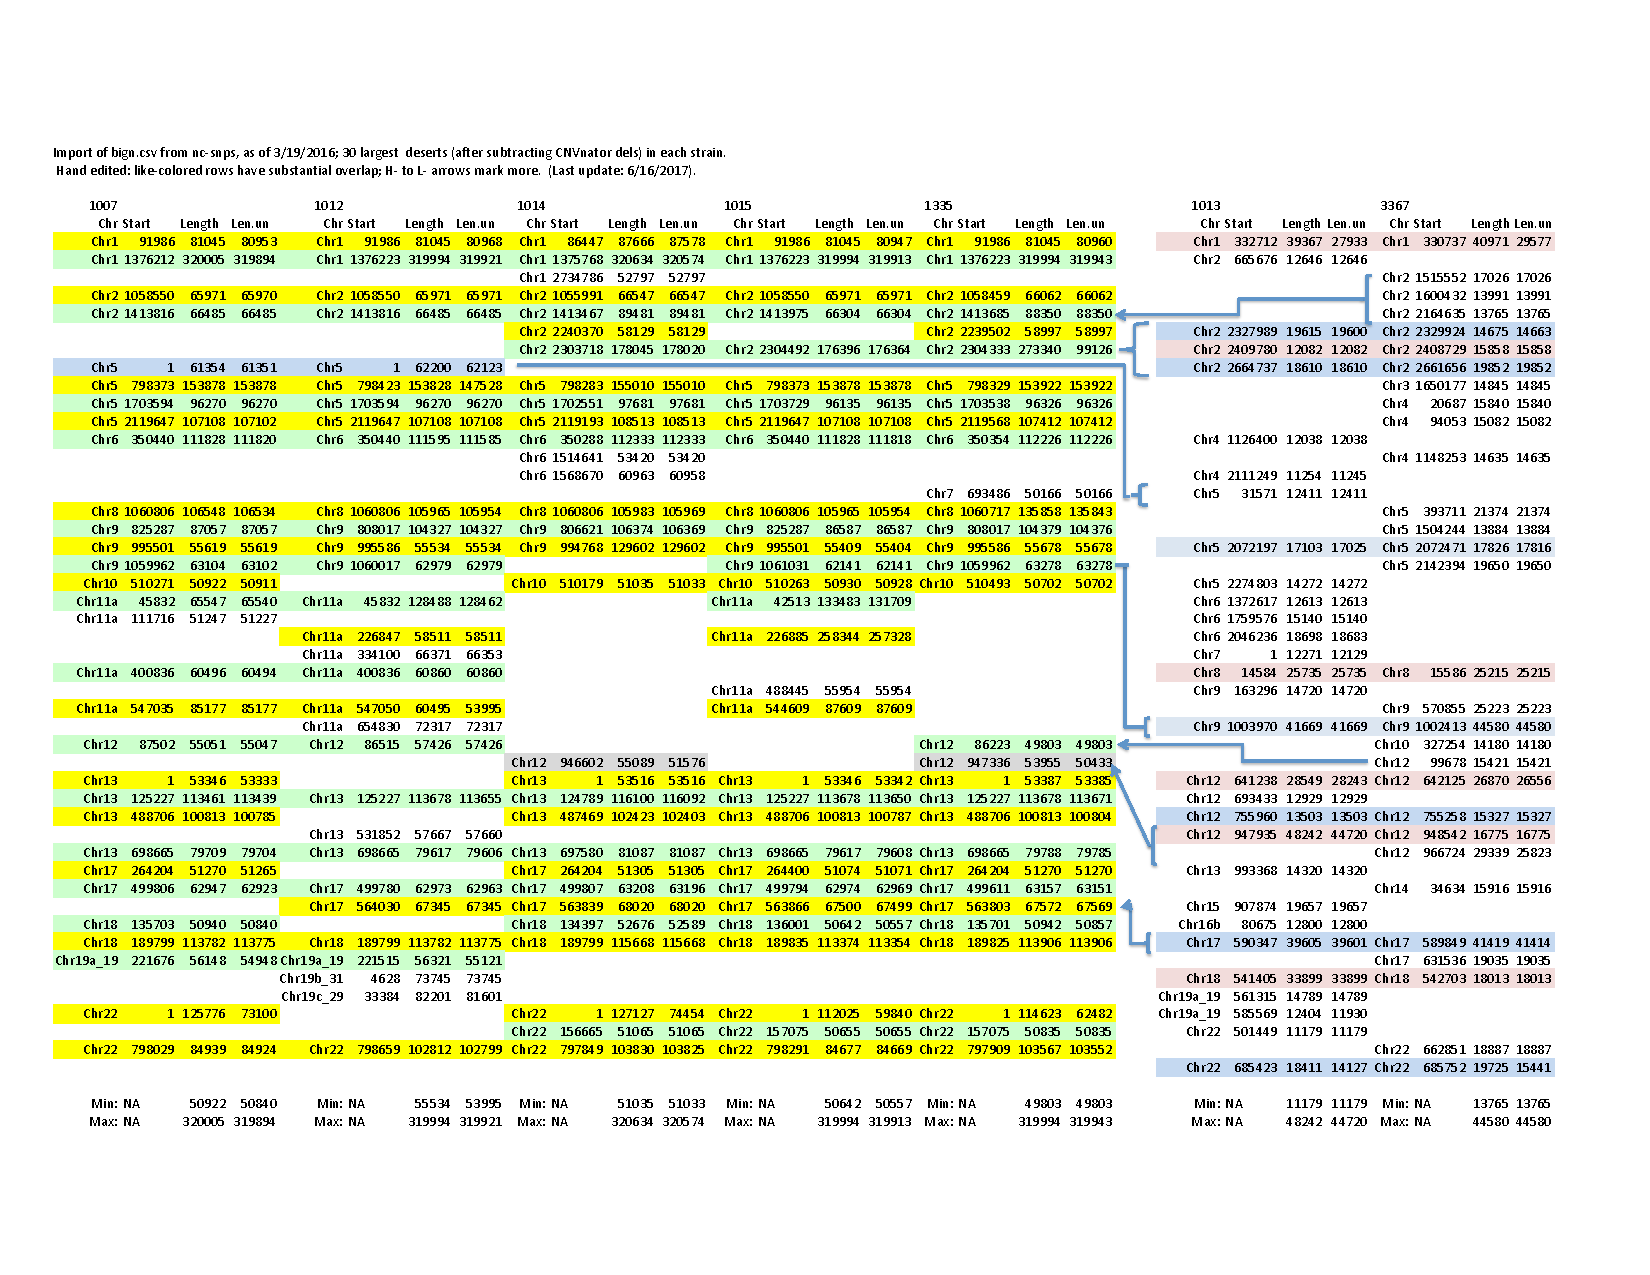
\includegraphics[trim=25 71 47 71,clip,scale=0.95,angle=90]{bign-xlsx.pdf}}
  \end{center}
  \caption{30 largest deserts}
  \label{fig:excel}
\end{figure}

Proposed fig for paper:  This does NOT bother to separate non-exonic SNPs.  I think the desert sizes, consistent exonic fraction, small ratio of non-exonic to exonic snp rates ($<1.5$x), and large ratio of nondesert to big-desert snp rates ($\approx 9$x) makes that refinement unnecessary, but we could do it; picture won't change much.

\begin{knitrout}\footnotesize
\definecolor{shadecolor}{rgb}{0.969, 0.969, 0.969}\color{fgcolor}\begin{kframe}
\begin{alltt}
  \hlstd{des.vs.non} \hlkwb{<-} \hlkwa{function}\hlstd{(}\hlkwc{fig.file.path}\hlstd{,} \hlkwc{strain}\hlstd{=}\hlnum{7}\hlstd{,} \hlkwc{length.thresh}\hlstd{=}\hlnum{50000}\hlstd{,}
                         \hlkwc{length.thresh.eff}\hlstd{=T,} \hlkwc{nc}\hlstd{=F,} \hlkwc{yclip}\hlstd{=}\hlkwa{NULL}\hlstd{,}
                         \hlkwc{xlab}\hlstd{=}\hlkwa{NULL}\hlstd{,} \hlkwc{ylab}\hlstd{=}\hlkwa{NULL}\hlstd{,} \hlkwc{ylab.sub}\hlstd{=}\hlkwa{NULL}\hlstd{,} \hlkwc{main}\hlstd{=}\hlkwa{NULL}\hlstd{,} \hlkwc{legend}\hlstd{=}\hlkwa{NULL}\hlstd{,} \hlkwc{panel}\hlstd{=}\hlkwa{NULL}\hlstd{,}
                         \hlkwc{des.col}\hlstd{=}\hlstr{'dodgerblue2'}\hlstd{,}
                         \hlkwc{cnv.dels}\hlstd{=cnv.dels.08.full,} \hlkwc{des.tables}\hlstd{=des,} \hlkwc{snp.tables}\hlstd{=snp.tables.full)\{}
    \hlkwd{pdf}\hlstd{(fig.file.path,}\hlkwc{width}\hlstd{=}\hlnum{6.5}\hlstd{,} \hlkwc{height}\hlstd{=}\hlnum{2.1}\hlstd{)} \hlcom{# was 3.1}
    \hlcom{# par seemingly must be set via par, after pdf() call.}
    \hlstd{opar} \hlkwb{<-} \hlkwd{par}\hlstd{(}\hlkwc{no.readonly}\hlstd{=}\hlnum{TRUE}\hlstd{,}\hlkwc{oma}\hlstd{=}\hlkwd{c}\hlstd{(}\hlnum{0}\hlstd{,}\hlnum{0}\hlstd{,}\hlnum{0}\hlstd{,}\hlnum{0}\hlstd{),}\hlkwc{mar}\hlstd{=}\hlkwd{c}\hlstd{(}\hlnum{3}\hlstd{,}\hlnum{3}\hlstd{,}\hlnum{1}\hlstd{,}\hlnum{1}\hlstd{),}\hlkwc{tcl}\hlstd{=}\hlopt{-}\hlnum{0.2}\hlstd{)}
    \hlkwd{on.exit}\hlstd{(}\hlkwd{par}\hlstd{(opar))}
    \hlstd{xx} \hlkwb{<-} \hlkwd{snp.rates}\hlstd{(}\hlkwc{strain}\hlstd{=strain,} \hlkwc{length.thresh}\hlstd{=length.thresh,}
                    \hlkwc{length.thresh.eff}\hlstd{=length.thresh.eff,} \hlkwc{nc}\hlstd{=nc,} \hlkwc{yclip}\hlstd{=yclip,}
                    \hlkwc{xlab}\hlstd{=xlab,} \hlkwc{ylab}\hlstd{=ylab,} \hlkwc{ylab.sub}\hlstd{=ylab.sub,} \hlkwc{main}\hlstd{=main,} \hlkwc{legend}\hlstd{=legend,}
                    \hlkwc{des.col}\hlstd{=des.col,}
                    \hlkwc{cnv.dels}\hlstd{=cnv.dels,} \hlkwc{des.tables}\hlstd{=des.tables,} \hlkwc{snp.tables}\hlstd{=snp.tables)}
    \hlkwa{if}\hlstd{(}\hlopt{!}\hlkwd{is.null}\hlstd{(panel))\{}
      \hlkwd{text}\hlstd{(}\hlnum{0.62}\hlstd{,}\hlnum{0.0092}\hlstd{,panel,}\hlkwc{cex}\hlstd{=}\hlnum{1.1}\hlstd{)} \hlcom{# for 2B, coords empirically set to roughly match rel pos in panel 2A}
    \hlstd{\}}
    \hlkwd{dev.off}\hlstd{()}
    \hlkwd{return}\hlstd{(xx)}
  \hlstd{\}}
\end{alltt}
\end{kframe}
\end{knitrout}

{\footnotesize Hmmm...; I tried ``dodgerblue2'' to match fig 2A, but it looks a fair bit paler in this context, so back to ``blue''}
%source(''../../../R/wlr.R')

%old way:
\begin{knitrout}\footnotesize
\definecolor{shadecolor}{rgb}{0.969, 0.969, 0.969}\color{fgcolor}\begin{kframe}
\begin{alltt}
\hlkwa{if}\hlstd{(}\hlkwd{exists}\hlstd{(}\hlstr{'snp.tables.full'}\hlstd{))\{}
  \hlstd{xx} \hlkwb{<-} \hlkwd{des.vs.non}\hlstd{(}\hlstr{'figs-mine/bigdes-snpdens-ny--Fig2Bproto.pdf'}\hlstd{,} \hlkwc{strain}\hlstd{=}\hlnum{7}\hlstd{,} \hlkwc{length.thresh}\hlstd{=}\hlnum{50000}\hlstd{,}
                   \hlkwc{length.thresh.eff}\hlstd{=T,} \hlkwc{nc}\hlstd{=F,} \hlkwc{yclip}\hlstd{=}\hlnum{0.01}\hlstd{,}
                   \hlkwc{xlab}\hlstd{=}\hlstr{'Desert Index'}\hlstd{,} \hlkwc{ylab}\hlstd{=}\hlstr{'SNP Density'}\hlstd{,}
                   \hlkwc{ylab.sub}\hlstd{=}\hlkwd{list}\hlstd{(}\hlkwc{text}\hlstd{=}\hlstr{'(SNPS / bp)'}\hlstd{,} \hlkwc{line}\hlstd{=}\hlnum{1.1}\hlstd{,} \hlkwc{cex}\hlstd{=}\hlnum{.75}\hlstd{),}
                   \hlkwc{main}\hlstd{=}\hlstr{''}\hlstd{,} \hlkwc{legend}\hlstd{=}\hlstr{''}\hlstd{,} \hlkwc{panel}\hlstd{=}\hlstr{'B'}\hlstd{,}  \hlkwc{des.col}\hlstd{=}\hlstr{'blue3'}\hlstd{,}
                   \hlkwc{cnv.dels}\hlstd{=cnv.dels.08.full,} \hlkwc{des.tables}\hlstd{=des,} \hlkwc{snp.tables}\hlstd{=snp.tables.full)}
  \hlkwd{print}\hlstd{(xx)}
\hlstd{\}}
\end{alltt}
\begin{verbatim}
# snp.rates:
#                                   Type SNP.count Total.Positions    SNP.Rate
# 1                          total snps:    158343        32610006 0.004855657
# 2           after removing NAs in ref:    158325        32381187 0.004889413
# 3 after (also) removing CNVnator dels:    158029        30940466 0.005107518
# $desert.stats
#        Chr   Start     End   iStart     iEnd  sn          snr         snsig  Length Len.eff
# 1     Chr1   91986  173030    91986   173030  15 0.0001852973 0.00004783912   81045   80951
# 2     Chr1 1376223 1696216  1376223  1696216  44 0.0001375550 0.00002073577  319994  319872
# 3     Chr2 1058459 1124520  4101044  4167105  35 0.0005298134 0.00008953108   66062   66061
# 4     Chr2 1413685 1502034  4456270  4544619  42 0.0004753820 0.00007333560   88350   88350
# 5     Chr2 2239502 2298498  5282087  5341083  38 0.0006441005 0.00010445325   58997   58997
# 6     Chr2 2304333 2577672  5346918  5620257  31 0.0003128090 0.00005617337  273340   99102
# 7     Chr5  798329  952250 11390484 11544405  23 0.0001494263 0.00003115522  153922  153922
# 8     Chr5 1703538 1799863 12295693 12392018  21 0.0002180097 0.00004756843   96326   96326
# 9     Chr5 2119568 2226979 12711723 12819134  13 0.0001210361 0.00003356733  107412  107406
# 10    Chr6  350354  462579 13248481 13360706  27 0.0002406031 0.00004629852  112226  112218
# 11    Chr7  693486  743651 15663093 15713258  48 0.0009568233 0.00013803947   50166   50166
# 12    Chr8 1060717 1196574 18022758 18158615  37 0.0002723953 0.00004477541  135858  135832
# 13    Chr9  808017  912395 19037256 19141634  29 0.0002778496 0.00005158821  104379  104373
# 14    Chr9  995586 1051263 19224825 19280502  13 0.0002334854 0.00006474964   55678   55678
# 15    Chr9 1059962 1123239 19289201 19352478  17 0.0002686643 0.00006515190   63278   63276
# 16   Chr10  510493  561194 19930792 19981493  19 0.0003748200 0.00008597349   50702   50691
# 17   Chr12  947336 1001290 22362288 22416242  27 0.0005354062 0.00010301139   53955   50429
# 18   Chr13       1   53387 22543335 22596721  20 0.0003747143 0.00008377296   53387   53374
# 19   Chr13  125227  238904 22668561 22782238  17 0.0001495742 0.00003627435  113678  113656
# 20   Chr13  488706  589518 23032040 23132852  40 0.0003968884 0.00006274111  100813  100784
# 21   Chr13  698665  778452 23241999 23321786  36 0.0004512239 0.00007518702   79788   79783
# 22   Chr17  264204  315473 26418797 26470066  32 0.0006242075 0.00011031090   51270   51265
# 23   Chr17  499611  562767 26654204 26717360  11 0.0001742353 0.00005252936   63157   63133
# 24   Chr17  563803  631374 26718396 26785967  16 0.0002368090 0.00005919524   67572   67565
# 25   Chr18  135701  186642 26950218 27001159  11 0.0002163778 0.00006523331   50942   50837
# 26   Chr18  189825  303730 27004342 27118247  28 0.0002458318 0.00004645214  113906  113899
# 27   Chr22       1  114623 29491915 29606537  18 0.0002905710 0.00006847828  114623   61947
# 28   Chr22  157075  207909 29648989 29699823  15 0.0002950723 0.00007617610   50835   50835
# 29   Chr22  797909  901475 30289823 30393389  33 0.0003187451 0.00005547756  103567  103531
# 30 Overall      NA      NA       NA       NA 756 0.0002902937            NA 2835228 2604259
# 
# $nondesert.stats
#      usnlen    usn        usnr        usnsig
# 1     90682    590 0.006506253 0.00026698538
# 2   1189188   7282 0.006123506 0.00007153870
# 3   2403965  13742 0.005716389 0.00004862414
# 4    289135   1473 0.005094506 0.00013240111
# 5    737390   4440 0.006021237 0.00009009129
# 6      5818     33 0.005672052 0.00098457335
# 7   5657400  32032 0.005661965 0.00003154585
# 8    751220   4694 0.006248502 0.00009091662
# 9    318373   1749 0.005493556 0.00013099734
# 10   105050    485 0.004616849 0.00020915582
# 11  2297937  11854 0.005158540 0.00004725756
# 12  2304222  12517 0.005432202 0.00004842203
# 13   878430   3942 0.004487552 0.00007131395
# 14    83163    430 0.005170569 0.00024870149
# 15     8698     70 0.008047827 0.00095802090
# 16   577907   3938 0.006814245 0.00010821691
# 17  2342395  12900 0.005507184 0.00004835435
# 18   125590    687 0.005470181 0.00020812882
# 19    71838    509 0.007085387 0.00031293966
# 20   249791   1463 0.005856896 0.00015267567
# 21   109140    803 0.007357522 0.00025868441
# 22  3065504  18033 0.005882556 0.00004367681
# 23   184095    857 0.004655205 0.00015864822
# 24     1035     17 0.016425121 0.00395082529
# 25   164228    929 0.005656770 0.00018506693
# 26     3182     29 0.009113765 0.00168465402
# 27  1671450   9694 0.005799755 0.00005873474
# 28    42451     62 0.001460507 0.00018534913
# 29   555092   2507 0.004516368 0.00008999725
# 30   810677   5071 0.006255266 0.00008756617
# 31 27095046 152832 0.005640588            NA
# 
# $merged.desert.stats
# NULL
\end{verbatim}
\end{kframe}
\end{knitrout}
%new way:
\begin{knitrout}\footnotesize
\definecolor{shadecolor}{rgb}{0.969, 0.969, 0.969}\color{fgcolor}\begin{kframe}
\begin{alltt}
\hlkwa{if}\hlstd{(}\hlkwd{exists}\hlstd{(}\hlstr{'snp.tables.full'}\hlstd{))\{}
  \hlstd{snp.rates.blob} \hlkwb{<-} \hlkwd{snp.rates.calc}\hlstd{(}\hlkwc{strain}\hlstd{=}\hlnum{7}\hlstd{,} \hlkwc{length.thresh}\hlstd{=}\hlnum{50000}\hlstd{,} \hlkwc{length.thresh.eff}\hlstd{=T,} \hlkwc{nc}\hlstd{=F,}
                                   \hlkwc{merge.thresh}\hlstd{=}\hlkwa{NULL}\hlstd{,} \hlkwc{snp.tables}\hlstd{=snp.tables.full,} \hlkwc{des.tables}\hlstd{=des,}
                                   \hlkwc{cnv.dels}\hlstd{=cnv.dels.08.full)}
  \hlstd{Description} \hlkwb{<-} \hlstr{'This .rda contains snp.rates.blob and cnv.dels.08.full; see nc-snps.rnw.'}
  \hlkwd{save}\hlstd{(Description, snp.rates.blob, cnv.dels.08.full,} \hlkwc{file}\hlstd{=}\hlstr{'Fig2B-data.rda'}\hlstd{)}
\hlstd{\}}
\end{alltt}
\begin{verbatim}
# snp.rates:
#                                   Type SNP.count Total.Positions    SNP.Rate
# 1                          total snps:    158343        32610006 0.004855657
# 2           after removing NAs in ref:    158325        32381187 0.004889413
# 3 after (also) removing CNVnator dels:    158029        30940466 0.005107518
\end{verbatim}
\end{kframe}
\end{knitrout}
\begin{knitrout}\footnotesize
\definecolor{shadecolor}{rgb}{0.969, 0.969, 0.969}\color{fgcolor}\begin{kframe}
\begin{alltt}
\hlkwa{if}\hlstd{(}\hlkwd{exists}\hlstd{(}\hlstr{'snp.tables.full'}\hlstd{))\{}
  \hlstd{xx} \hlkwb{<-} \hlkwd{snp.rates.plot}\hlstd{(snp.rates.blob,} \hlkwc{des.col}\hlstd{=}\hlstr{'blue3'}\hlstd{,} \hlkwc{undes.col}\hlstd{=}\hlstr{'black'}\hlstd{,} \hlkwc{yclip}\hlstd{=}\hlnum{0.01}\hlstd{,} \hlkwc{legend}\hlstd{=}\hlstr{''}\hlstd{,}
                       \hlkwc{xlab}\hlstd{=}\hlstr{'Desert Index'}\hlstd{,} \hlkwc{ylab}\hlstd{=}\hlstr{'SNP Density'}\hlstd{,} \hlkwc{main}\hlstd{=}\hlstr{''}\hlstd{,}
                       \hlkwc{ylab.sub}\hlstd{=}\hlkwd{list}\hlstd{(}\hlkwc{text}\hlstd{=}\hlstr{'(SNPS / bp)'}\hlstd{,} \hlkwc{line}\hlstd{=}\hlnum{1.1}\hlstd{,} \hlkwc{cex}\hlstd{=}\hlnum{.75}\hlstd{))}
  \hlcom{# panel='B':}
  \hlkwd{text}\hlstd{(}\hlnum{0.62}\hlstd{,}\hlnum{0.0092}\hlstd{,}\hlstr{'B'}\hlstd{,}\hlkwc{cex}\hlstd{=}\hlnum{1.1}\hlstd{)} \hlcom{# for 2B, coords empirically set to roughly match rel pos in panel 2A}
  \hlkwd{print}\hlstd{(xx)}
\hlstd{\}}
\end{alltt}
\end{kframe}
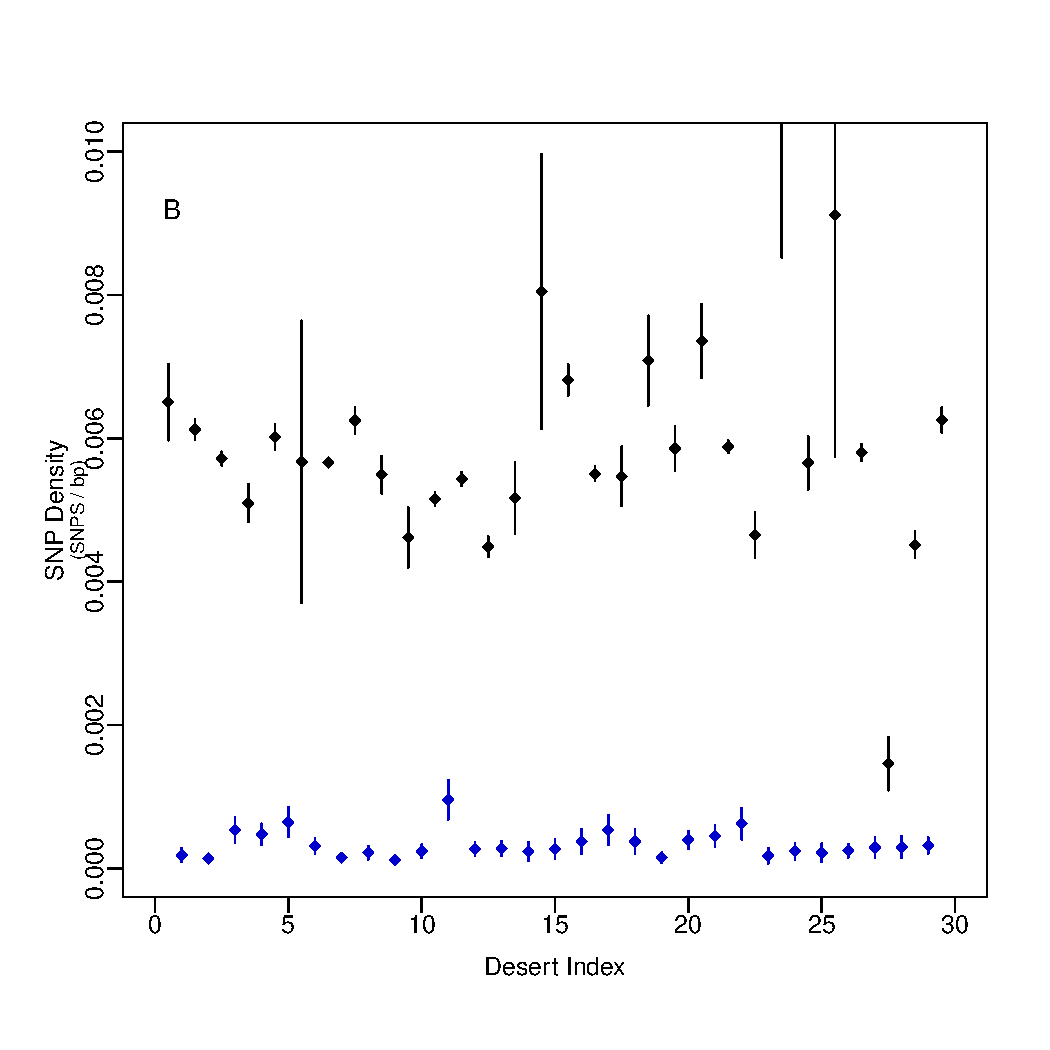
\includegraphics[width=\maxwidth]{figs-knitr/unnamed-chunk-9-1} 
\begin{kframe}\begin{verbatim}
# $desert.stats
#        Chr   Start     End   iStart     iEnd  sn          snr         snsig  Length Len.eff
# 1     Chr1   91986  173030    91986   173030  15 0.0001852973 0.00004783912   81045   80951
# 2     Chr1 1376223 1696216  1376223  1696216  44 0.0001375550 0.00002073577  319994  319872
# 3     Chr2 1058459 1124520  4101044  4167105  35 0.0005298134 0.00008953108   66062   66061
# 4     Chr2 1413685 1502034  4456270  4544619  42 0.0004753820 0.00007333560   88350   88350
# 5     Chr2 2239502 2298498  5282087  5341083  38 0.0006441005 0.00010445325   58997   58997
# 6     Chr2 2304333 2577672  5346918  5620257  31 0.0003128090 0.00005617337  273340   99102
# 7     Chr5  798329  952250 11390484 11544405  23 0.0001494263 0.00003115522  153922  153922
# 8     Chr5 1703538 1799863 12295693 12392018  21 0.0002180097 0.00004756843   96326   96326
# 9     Chr5 2119568 2226979 12711723 12819134  13 0.0001210361 0.00003356733  107412  107406
# 10    Chr6  350354  462579 13248481 13360706  27 0.0002406031 0.00004629852  112226  112218
# 11    Chr7  693486  743651 15663093 15713258  48 0.0009568233 0.00013803947   50166   50166
# 12    Chr8 1060717 1196574 18022758 18158615  37 0.0002723953 0.00004477541  135858  135832
# 13    Chr9  808017  912395 19037256 19141634  29 0.0002778496 0.00005158821  104379  104373
# 14    Chr9  995586 1051263 19224825 19280502  13 0.0002334854 0.00006474964   55678   55678
# 15    Chr9 1059962 1123239 19289201 19352478  17 0.0002686643 0.00006515190   63278   63276
# 16   Chr10  510493  561194 19930792 19981493  19 0.0003748200 0.00008597349   50702   50691
# 17   Chr12  947336 1001290 22362288 22416242  27 0.0005354062 0.00010301139   53955   50429
# 18   Chr13       1   53387 22543335 22596721  20 0.0003747143 0.00008377296   53387   53374
# 19   Chr13  125227  238904 22668561 22782238  17 0.0001495742 0.00003627435  113678  113656
# 20   Chr13  488706  589518 23032040 23132852  40 0.0003968884 0.00006274111  100813  100784
# 21   Chr13  698665  778452 23241999 23321786  36 0.0004512239 0.00007518702   79788   79783
# 22   Chr17  264204  315473 26418797 26470066  32 0.0006242075 0.00011031090   51270   51265
# 23   Chr17  499611  562767 26654204 26717360  11 0.0001742353 0.00005252936   63157   63133
# 24   Chr17  563803  631374 26718396 26785967  16 0.0002368090 0.00005919524   67572   67565
# 25   Chr18  135701  186642 26950218 27001159  11 0.0002163778 0.00006523331   50942   50837
# 26   Chr18  189825  303730 27004342 27118247  28 0.0002458318 0.00004645214  113906  113899
# 27   Chr22       1  114623 29491915 29606537  18 0.0002905710 0.00006847828  114623   61947
# 28   Chr22  157075  207909 29648989 29699823  15 0.0002950723 0.00007617610   50835   50835
# 29   Chr22  797909  901475 30289823 30393389  33 0.0003187451 0.00005547756  103567  103531
# 30 Overall      NA      NA       NA       NA 756 0.0002902937            NA 2835228 2604259
# 
# $nondesert.stats
#      usnlen    usn        usnr        usnsig
# 1     90682    590 0.006506253 0.00026698538
# 2   1189188   7282 0.006123506 0.00007153870
# 3   2403965  13742 0.005716389 0.00004862414
# 4    289135   1473 0.005094506 0.00013240111
# 5    737390   4440 0.006021237 0.00009009129
# 6      5818     33 0.005672052 0.00098457335
# 7   5657400  32032 0.005661965 0.00003154585
# 8    751220   4694 0.006248502 0.00009091662
# 9    318373   1749 0.005493556 0.00013099734
# 10   105050    485 0.004616849 0.00020915582
# 11  2297937  11854 0.005158540 0.00004725756
# 12  2304222  12517 0.005432202 0.00004842203
# 13   878430   3942 0.004487552 0.00007131395
# 14    83163    430 0.005170569 0.00024870149
# 15     8698     70 0.008047827 0.00095802090
# 16   577907   3938 0.006814245 0.00010821691
# 17  2342395  12900 0.005507184 0.00004835435
# 18   125590    687 0.005470181 0.00020812882
# 19    71838    509 0.007085387 0.00031293966
# 20   249791   1463 0.005856896 0.00015267567
# 21   109140    803 0.007357522 0.00025868441
# 22  3065504  18033 0.005882556 0.00004367681
# 23   184095    857 0.004655205 0.00015864822
# 24     1035     17 0.016425121 0.00395082529
# 25   164228    929 0.005656770 0.00018506693
# 26     3182     29 0.009113765 0.00168465402
# 27  1671450   9694 0.005799755 0.00005873474
# 28    42451     62 0.001460507 0.00018534913
# 29   555092   2507 0.004516368 0.00008999725
# 30   810677   5071 0.006255266 0.00008756617
# 31 27095046 152832 0.005640588            NA
# 
# $merged.desert.stats
# NULL
\end{verbatim}
\end{kframe}
\end{knitrout}

Show fig juxtaposed with Fig2a for comparison as Fig~\ref{fig:2a2b}.  (Surrounding boxes just to make marginal space obvious; change fbox to mbox to remove.)
\begin{figure}
  \begin{center}
    \fbox{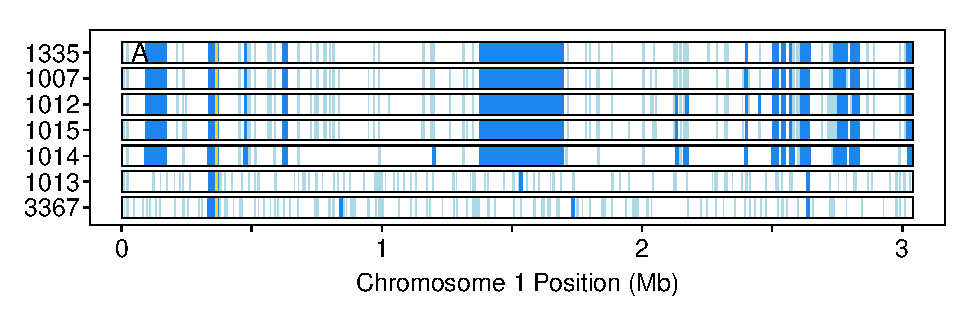
\includegraphics{../paperfigs/Fig2A-desert-distribution-figs-mine/Fig2A-desert-distribution-figq.pdf}}\\
    \fbox{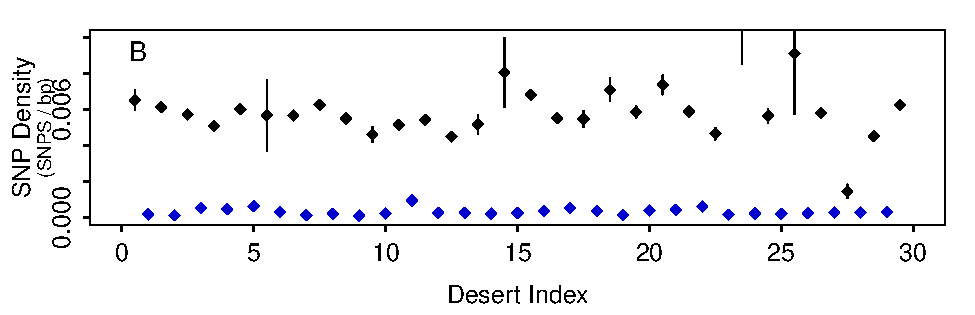
\includegraphics{figs-mine/bigdes-snpdens-ny--Fig2Bproto.pdf}}
  \end{center}
  \caption{Proposed caption: Attributes of SNP deserts for {\it T. pseudonana\/} isolates. A) SNP distributions across the 3 Mb of Chromosome 1 for the seven {\it T. pseudonana\/} isolates. Regions in blue have significantly low SNP density (``SNP deserts'') based on a negative binomial model (Methods). Pink(???) region is a gap of known size in the reference sequence. The large region centered near 1.5Mb is a 320Kb SNP desert present in all L-isolates but neither H-isolate. B) SNP densities (SNP per base-pair---$\mu\pm2\sigma$) in the 29 deserts that span at least 50Kb of the CCMP 1335 genome (blue) and the thirty regions surrounding these deserts (including deserts smaller than 50Kb; black).  }
  \label{fig:2a2b}
\end{figure}

For comparison, here's an analogous plot for Italy (except needed to lower thresh to find any deserts; code breaks if none) :

\begin{knitrout}\footnotesize
\definecolor{shadecolor}{rgb}{0.969, 0.969, 0.969}\color{fgcolor}\begin{kframe}
\begin{alltt}
\hlkwa{if}\hlstd{(}\hlkwd{exists}\hlstd{(}\hlstr{'snp.tables.full'}\hlstd{))\{}
  \hlstd{xx} \hlkwb{<-} \hlkwd{des.vs.non}\hlstd{(}\hlstr{'figs-mine/bigdes-snpdens-it.pdf'}\hlstd{,} \hlkwc{strain}\hlstd{=}\hlnum{6}\hlstd{,}
                   \hlkwc{length.thresh}\hlstd{=}\hlnum{25000}\hlstd{,} \hlkwc{length.thresh.eff}\hlstd{=T,} \hlkwc{nc}\hlstd{=F,} \hlkwc{yclip}\hlstd{=}\hlnum{0.01}\hlstd{)}
  \hlkwd{print}\hlstd{(xx)}
\hlstd{\}}
\end{alltt}
\begin{verbatim}
# snp.rates:
#                                   Type SNP.count Total.Positions    SNP.Rate
# 1                          total snps:    246773        32610006 0.007567401
# 2           after removing NAs in ref:    246757        32381187 0.007620382
# 3 after (also) removing CNVnator dels:    244530        31976174 0.007647256
# $desert.stats
#       Chr   Start     End   iStart     iEnd  sn          snr         snsig Length Len.eff
# 1    Chr1  330737  371707   330737   371707  17 0.0005758808 0.00013963138  40971   29520
# 2    Chr8   15586   40800 16977627 17002841  27 0.0010707912 0.00020596350  25215   25215
# 3    Chr9  570855  596077 18800094 18825316  47 0.0018635264 0.00027156987  25223   25221
# 4    Chr9 1002413 1046992 19231652 19276231  23 0.0005159264 0.00010755034  44580   44580
# 5   Chr12  642125  668994 22057077 22083946  31 0.0011673445 0.00020953885  26870   26556
# 6   Chr12  966724  996062 22381676 22411014  31 0.0012004802 0.00021548315  29339   25823
# 7   Chr17  589849  631267 26744442 26785860  12 0.0002897851 0.00008364162  41419   41410
# 8 Overall      NA      NA       NA       NA 188 0.0008611016            NA 233617  218325
# 
# $nondesert.stats
#     usnlen    usn        usnr        usnsig
# 1   300917   2548 0.008467451 0.00016703461
# 2 16485058 123688 0.007503037 0.00002125386
# 3  1787629  15685 0.008774192 0.00006975112
# 4   406279   2995 0.007371781 0.00013420458
# 5  2699187  20858 0.007727512 0.00005329897
# 6   287730   2162 0.007513989 0.00016099222
# 7  4253468  34101 0.008017223 0.00004324067
# 8  4299631  35946 0.008360252 0.00004391077
# 9 30519899 237983 0.007797634            NA
# 
# $merged.desert.stats
# NULL
\end{verbatim}
\end{kframe}
\end{knitrout}

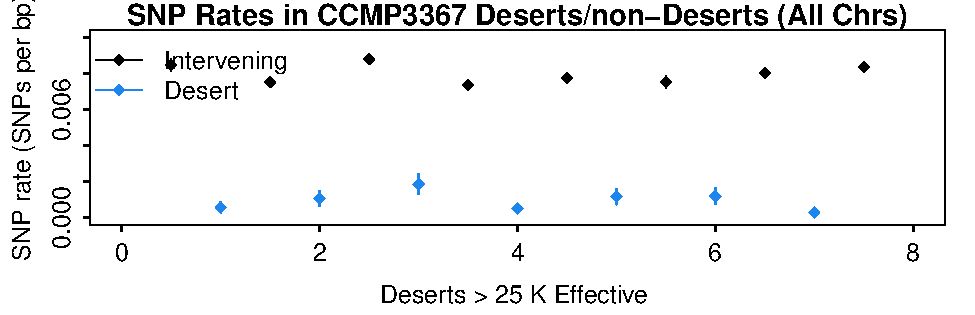
\includegraphics{figs-mine/bigdes-snpdens-it.pdf}

In the NY plot, inter-desert region \#28 had unusually low SNP rate.  Fig below is that region ($\pm5$K).  Seems to be a SNP-free region of normal coverage with 2--4 interspersed regions of 2x -- 4x coverage, probably assembly errors (collapsed repeats), with ``SNPs'' that are actually copy-to-copy differences.  CNVnator calls 2--4 high-coverage patches there, and we call two shorter deserts in that interval, spanning approximately 36Kb of the 45Kb region.  This doesn't fundamentally challenge our story that the big deserts are much younger than nondeserts.  Here are CNVnator and desert calls in the vicinity:

\begin{knitrout}\footnotesize
\definecolor{shadecolor}{rgb}{0.969, 0.969, 0.969}\color{fgcolor}\begin{kframe}
\begin{alltt}
\hlstd{cnv.chronly[cnv.chronly}\hlopt{$}\hlstd{strain}\hlopt{==}\hlstr{'tp1335'} \hlopt{&} \hlstd{cnv.chronly}\hlopt{$}\hlstd{chr}\hlopt{==}\hlstr{'Chr22'} \hlopt{&} \hlstd{cnv.chronly}\hlopt{$}\hlstd{start} \hlopt{<} \hlnum{211000}\hlstd{,]}
\end{alltt}
\begin{verbatim}
#      strain   chr  start    end length filtered     type cov_ratio   dup_frac   iStart     iEnd
# 1931 tp1335 Chr22      1  55800  55800     TRUE CNVnator  0.545751 0.99414600 29491915 29547714
# 1932 tp1335 Chr22 112601 115500   2900    FALSE CNVnator  1.682160 0.45551500 29604515 29607414
# 1933 tp1335 Chr22 123701 130800   7100    FALSE CNVnator  2.343170 0.55210400 29615615 29622714
# 1934 tp1335 Chr22 152501 159200   6700    FALSE CNVnator  2.166130 0.00682793 29644415 29651114
# 1935 tp1335 Chr22 210101 217100   7000    FALSE CNVnator  4.942700 0.25746200 29702015 29709014
\end{verbatim}
\begin{alltt}
\hlstd{des.df[[}\hlnum{7}\hlstd{]][des.df[[}\hlnum{7}\hlstd{]]}\hlopt{$}\hlstd{Chr}\hlopt{==}\hlstr{'Chr22'} \hlopt{&} \hlstd{des.df[[}\hlnum{7}\hlstd{]]}\hlopt{$}\hlstd{Start} \hlopt{<} \hlnum{211000}\hlstd{,]}
\end{alltt}
\begin{verbatim}
#        Chr  Start    End Length   iStart     iEnd
# 1102 Chr22      1 114623 114623 29491915 29606537
# 2102 Chr22 115060 125973  10914 29606974 29617887
# 3102 Chr22 128188 153417  25230 29620102 29645331
# 4102 Chr22 157075 207909  50835 29648989 29699823
\end{verbatim}
\end{kframe}
\end{knitrout}

\begin{knitrout}\scriptsize
\definecolor{shadecolor}{rgb}{0.969, 0.969, 0.969}\color{fgcolor}\begin{kframe}
\begin{alltt}
\hlstd{iBeg} \hlkwb{<-} \hlnum{29606538}
\hlstd{iEnd} \hlkwb{<-} \hlnum{29648988}
\hlkwd{seechunk}\hlstd{(}\hlnum{7}\hlstd{,(iBeg}\hlopt{+}\hlstd{iEnd)}\hlopt{/}\hlnum{2}\hlstd{,(iEnd}\hlopt{-}\hlstd{iBeg)}\hlopt{/}\hlnum{2}\hlopt{+}\hlnum{5000}\hlstd{,}\hlkwc{snp.tables}\hlstd{=snp.tables.full,}\hlkwc{ymax}\hlstd{=}\hlnum{400}\hlstd{)}
\end{alltt}
\end{kframe}

{\centering 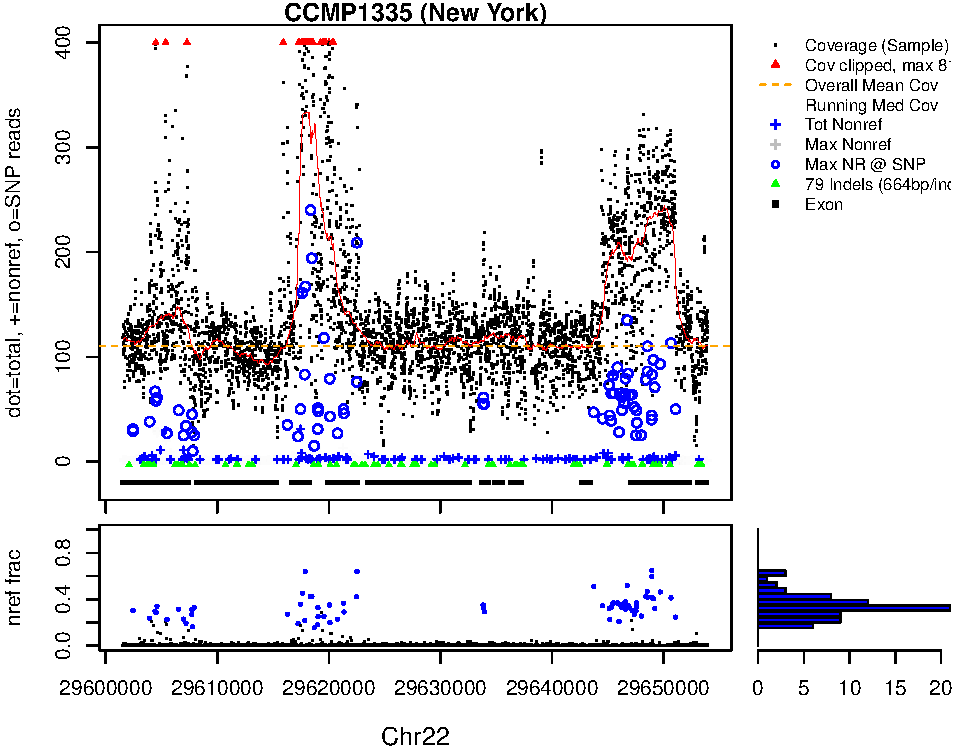
\includegraphics[width=\maxwidth]{figs-knitr/ch22-undes-1} 

}



\end{knitrout}

For comparison, here are all 1335 deserts with $>25$Kb non-exonic.  Advantages: (A) point 28 goes away, (B) $2\sigma$ error bars are slightly more visible so there is (somewhat) better evidence that these have concordant snp rates.  Disadvantages: (A) slightly harder to explain, (B) intervening rates at 8, 12 drop,  (C) fewer points, (D) need to look at H-clade, too, to pick an nc-length threshold that is clearly above theirs; 25k is probably in the ballpark, but I have not checked.

\begin{knitrout}\footnotesize
\definecolor{shadecolor}{rgb}{0.969, 0.969, 0.969}\color{fgcolor}\begin{kframe}
\begin{alltt}
\hlkwa{if}\hlstd{(}\hlkwd{exists}\hlstd{(}\hlstr{'snp.tables.full'}\hlstd{))\{}
  \hlstd{xx} \hlkwb{<-} \hlkwd{des.vs.non}\hlstd{(}\hlstr{'figs-mine/bigdes-snpdens-nc-ny.pdf'}\hlstd{,} \hlkwc{strain}\hlstd{=}\hlnum{7}\hlstd{,}
                   \hlkwc{length.thresh}\hlstd{=}\hlnum{25000}\hlstd{,} \hlkwc{length.thresh.eff}\hlstd{=T,} \hlkwc{nc}\hlstd{=T)}
  \hlkwd{print}\hlstd{(xx)}
\hlstd{\}}
\end{alltt}
\begin{verbatim}
# snp.rates:
#                                   Type SNP.count Total.Positions    SNP.Rate
# 1                          total snps:    158343        32610006 0.004855657
# 2           after removing NAs in ref:    158325        32381187 0.004889413
# 3 after (also) removing CNVnator dels:    158029        30940466 0.005107518
# 4         after (also) removing exons:     77081        12970363 0.005942856
# $desert.stats
#        Chr   Start     End   iStart     iEnd  sn           snr         snsig  Length Len.eff
# 1     Chr1   91986  173030    91986   173030   7 0.00020186873 0.00007629151   81045   34676
# 2     Chr1 1376223 1696216  1376223  1696216  20 0.00015547626 0.00003476285  319994  128637
# 3     Chr2 1413685 1502034  4456270  4544619  23 0.00071852546 0.00014976908   88350   32010
# 4     Chr2 2304333 2577672  5346918  5620257  15 0.00038308305 0.00009889267  273340   39156
# 5     Chr5  798329  952250 11390484 11544405   8 0.00013922002 0.00004921828  153922   57463
# 6     Chr5 1703538 1799863 12295693 12392018   9 0.00028246814 0.00009414275   96326   31862
# 7     Chr5 2119568 2226979 12711723 12819134   9 0.00022042616 0.00007346729  107412   40830
# 8     Chr6  350354  462579 13248481 13360706   9 0.00022624434 0.00007540625  112226   39780
# 9     Chr6 2033123 2066734 14931250 14964861  26 0.00087289331 0.00017111373   33612   29786
# 10    Chr8 1060717 1196574 18022758 18158615  16 0.00029198679 0.00007298604  135858   54797
# 11    Chr9  808017  912395 19037256 19141634  15 0.00037852024 0.00009771501  104379   39628
# 12    Chr9 1059962 1123239 19289201 19352478  10 0.00039785160 0.00012578669   63278   25135
# 13   Chr12  947336 1001290 22362288 22416242  17 0.00060055817 0.00014561301   53955   28307
# 14   Chr13       1   53387 22543335 22596721  15 0.00049136830 0.00012683957   53387   30527
# 15   Chr13  125227  238904 22668561 22782238   4 0.00009781147 0.00004890334  113678   40895
# 16   Chr13  488706  589518 23032040 23132852  17 0.00043936731 0.00010653881  100813   38692
# 17   Chr13  698665  778452 23241999 23321786  11 0.00027473214 0.00008282348   79788   40039
# 18   Chr17  563803  631374 26718396 26785967  11 0.00031713997 0.00009560614   67572   34685
# 19   Chr18  135701  186642 26950218 27001159   2 0.00007949442 0.00005620881   50942   25159
# 20   Chr18  189825  303730 27004342 27118247  19 0.00037386120 0.00008575361  113906   50821
# 21   Chr22       1  114623 29491915 29606537  14 0.00044574631 0.00011910416  114623   31408
# 22   Chr22  797909  901475 30289823 30393389  25 0.00066521207 0.00013299816  103567   37582
# 23 Overall      NA      NA       NA       NA 302 0.00033118574            NA 2421973  911875
# 
# $nondesert.stats
#      usnlen   usn        usnr        usnsig
# 1     46701   337 0.007216120 0.00039166623
# 2    427797  3160 0.007386681 0.00013091694
# 3   1018670  6695 0.006572295 0.00008005895
# 4    318463  2239 0.007030644 0.00014805940
# 5   2129498 15121 0.007100735 0.00005753944
# 6    266626  1936 0.007261107 0.00016442494
# 7    109786   745 0.006785929 0.00024777222
# 8     57193   212 0.003706747 0.00025410818
# 9    566026  3629 0.006411366 0.00010608657
# 10  1158839  7592 0.006551385 0.00007494242
# 11   352181  1900 0.005394953 0.00012343440
# 12    69050   276 0.003997104 0.00024011603
# 13  1253524  8185 0.006529592 0.00007193730
# 14    51540   322 0.006247575 0.00034707443
# 15    37812   308 0.008145562 0.00046224229
# 16    86093   638 0.007410591 0.00029229899
# 17    31554   351 0.011123788 0.00059043229
# 18  1359491  9254 0.006806959 0.00007051885
# 19    92523   487 0.005263556 0.00023788595
# 20     1098    11 0.010018215 0.00300543683
# 21   701458  4834 0.006891361 0.00009877568
# 22   296564  1333 0.004494814 0.00012283395
# 23   384840  2773 0.007205592 0.00013634035
# 24 10817327 72338 0.006687234            NA
# 
# $merged.desert.stats
# NULL
\end{verbatim}
\end{kframe}
\end{knitrout}

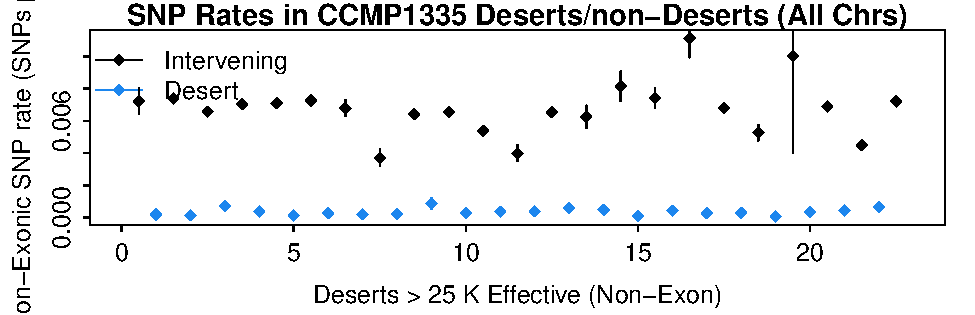
\includegraphics{figs-mine/bigdes-snpdens-nc-ny.pdf}

And comparable data for Italy, based on 10Kb non-exonic (a wild guess at a comparable threshold):

\begin{knitrout}\footnotesize
\definecolor{shadecolor}{rgb}{0.969, 0.969, 0.969}\color{fgcolor}\begin{kframe}
\begin{alltt}
\hlkwa{if}\hlstd{(}\hlkwd{exists}\hlstd{(}\hlstr{'snp.tables.full'}\hlstd{))\{}
  \hlstd{xx} \hlkwb{<-} \hlkwd{des.vs.non}\hlstd{(}\hlstr{'figs-mine/bigdes-snpdens-nc-it.pdf'}\hlstd{,} \hlkwc{strain}\hlstd{=}\hlnum{6}\hlstd{,}
                   \hlkwc{length.thresh}\hlstd{=}\hlnum{10000}\hlstd{,} \hlkwc{length.thresh.eff}\hlstd{=T,} \hlkwc{nc}\hlstd{=T)}
  \hlkwd{print}\hlstd{(xx)}
\hlstd{\}}
\end{alltt}
\begin{verbatim}
# snp.rates:
#                                   Type SNP.count Total.Positions    SNP.Rate
# 1                          total snps:    246773        32610006 0.007567401
# 2           after removing NAs in ref:    246757        32381187 0.007620382
# 3 after (also) removing CNVnator dels:    244530        31976174 0.007647256
# 4         after (also) removing exons:    124010        13291348 0.009330130
# $desert.stats
#        Chr   Start     End   iStart     iEnd  sn          snr        snsig Length Len.eff
# 1     Chr1  330737  371707   330737   371707  10 0.0007224911 0.0002283892  40971   13841
# 2     Chr2 2661656 2681507  5704241  5724092  15 0.0013321492 0.0003437303  19852   11260
# 3     Chr4   20687   36526  8210519  8226358  33 0.0025965851 0.0004514202  15840   12709
# 4     Chr4   94053  109134  8283885  8298966  30 0.0023257617 0.0004241300  15082   12899
# 5     Chr7       1   11920 14969608 14981527  16 0.0014265335 0.0003563789  11920   11216
# 6     Chr9 1002413 1046992 19231652 19276231  14 0.0007194245 0.0001922051  44580   19460
# 7    Chr10 1090040 1103502 20510339 20523801  12 0.0009079216 0.0002619754  13463   13217
# 8    Chr12  679161  691915 22094113 22106867  21 0.0020072644 0.0004375812  12755   10462
# 9    Chr12  755258  770584 22170210 22185536  12 0.0008773854 0.0002531682  15327   13677
# 10   Chr12  948542  965316 22363494 22380268  22 0.0021995601 0.0004684318  16775   10002
# 11   Chr12  966724  996062 22381676 22411014  22 0.0014510916 0.0003091492  29339   15161
# 12   Chr17  589849  631267 26744442 26785860  10 0.0004183225 0.0001322575  41419   23905
# 13   Chr17  631536  650570 26786129 26805163  31 0.0017828387 0.0003199217  19035   17388
# 14 Overall      NA      NA       NA       NA 248 0.0013391146           NA 296358  185197
# 
# $nondesert.stats
#      usnlen    usn        usnr        usnsig
# 1    124920   1364 0.010918988 0.00029402966
# 2   1959846  19848 0.010127326 0.00007151977
# 3    922688   8458 0.009166696 0.00009921544
# 4     32133    340 0.010581023 0.00057079256
# 5   2442814  22636 0.009266362 0.00006130387
# 6   1630801  16839 0.010325601 0.00007915956
# 7    448646   4525 0.010085903 0.00014917782
# 8    658232   5973 0.009074308 0.00011687936
# 9     20179    196 0.009713068 0.00069041294
# 10    76900    827 0.010754226 0.00037194482
# 11      473      2 0.004228330 0.00298355288
# 12  1706777  17372 0.010178248 0.00007682926
# 13      268      8 0.029850746 0.01039511927
# 14  1843524  19015 0.010314485 0.00007441286
# 15 11868201 117403 0.009892232            NA
# 
# $merged.desert.stats
# NULL
\end{verbatim}
\end{kframe}
\end{knitrout}

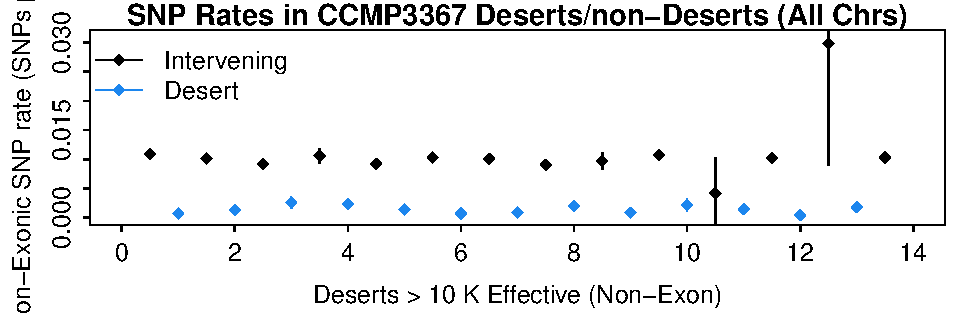
\includegraphics{figs-mine/bigdes-snpdens-nc-it.pdf}


\section{Small Deserts}
\label{sec:small-deserts}

A few disorganized thoughts on why I think the uniformity of the snp rate in the small deserts is potentially artifactual.  Avg snp rates, and avg distance to 5th snp are: 

\begin{knitrout}\footnotesize
\definecolor{shadecolor}{rgb}{0.969, 0.969, 0.969}\color{fgcolor}\begin{kframe}
\begin{alltt}
\hlstd{bppersnp} \hlkwb{<-} \hlkwd{genome.length.constants}\hlstd{()}\hlopt{$}\hlstd{genome.length.trunc}\hlopt{/}\hlstd{ddb.full}\hlopt{$}\hlstd{snp.tot}
\hlkwd{names}\hlstd{(bppersnp)} \hlkwb{<-} \hlkwd{names}\hlstd{(snp.tables.chr1)}
\hlkwd{rbind}\hlstd{(bppersnp,} \hlkwc{fifth}\hlstd{=}\hlnum{5}\hlopt{*}\hlstd{bppersnp)}
\end{alltt}
\begin{verbatim}
#              1007     1012     1013      1014     1015     3367     1335
# bppersnp 188.6638 182.9807 122.9541  340.4995 173.4747 126.8444 197.6834
# fifth    943.3191 914.9037 614.7706 1702.4977 867.3737 634.2222 988.4170
\end{verbatim}
\end{kframe}
\end{knitrout}
\noindent And so deserts aren't called until the 5th snp is about: 
\begin{knitrout}\footnotesize
\definecolor{shadecolor}{rgb}{0.969, 0.969, 0.969}\color{fgcolor}\begin{kframe}
\begin{alltt}
\hlstd{des.threshold} \hlkwb{<-} \hlkwd{qnbinom}\hlstd{(}\hlnum{1e-4}\hlstd{,}\hlnum{5}\hlstd{,}\hlnum{1}\hlopt{/}\hlstd{bppersnp,}\hlkwc{lower.tail}\hlstd{=F); des.threshold}
\end{alltt}
\begin{verbatim}
# 1007 1012 1013 1014 1015 3367 1335 
# 3343 3242 2175 6043 3073 2244 3504
\end{verbatim}
\end{kframe}
\end{knitrout}
\noindent base pairs away, which is about comparable to both the expected distance to the 5th and to the median desert lengths:
\begin{knitrout}\footnotesize
\definecolor{shadecolor}{rgb}{0.969, 0.969, 0.969}\color{fgcolor}\begin{kframe}
\begin{alltt}
\hlkwd{print}\hlstd{(}\hlkwd{rbind}\hlstd{(des.threshold,}
            \hlkwc{des.median}\hlstd{=dsum.df[,}\hlstr{'Median'}\hlstd{],}
            \hlkwc{des.thresh.over.expect}\hlstd{=des.threshold}\hlopt{/}\hlstd{(}\hlnum{5}\hlopt{*}\hlstd{bppersnp),}
            \hlkwc{des.median.over.des.thresh}\hlstd{=dsum.df[,}\hlstr{'Median'}\hlstd{]}\hlopt{/}\hlstd{des.threshold),}
      \hlkwc{digits}\hlstd{=}\hlnum{3}
\hlstd{)}
\end{alltt}
\begin{verbatim}
#                               1007    1012    1013     1014    1015    3367    1335
# des.threshold              3343.00 3242.00 2175.00  6043.00 3073.00 2244.00 3504.00
# des.median                 6515.00 6244.00 3500.50 10745.50 5859.00 3615.50 6484.00
# des.thresh.over.expect        3.54    3.54    3.54     3.55    3.54    3.54    3.55
# des.median.over.des.thresh    1.95    1.93    1.61     1.78    1.91    1.61    1.85
\end{verbatim}
\end{kframe}
\end{knitrout}

\noindent i.e., the threshold of desertness is about 3.5 times the expected distance to the 5th snp, and the median desert length is only about twice the threshold.  The later means that we can't pack very many snps into a short desert, and likewise it is hard to arrange for there to be very few, meaning the snp rate for short deserts can't vary too much.  Example: in 1335, with threshold $\approx 3500$, having zero snps in a span of $L+3500$, followed by a cluster of 5 creates a desert of length $L$, say for $L\approx7000$;  seemingly a more likely configuration is to have 5--10 snps sprinkled over a similar distance, but packing more in will greatly shorten or destroy the desert, unless they are all packed at the ends. 

Sprinkling SNPs at random, of course we would expect to see some patches where fewer snps land than expected, AND genomes tend to be more heterogeneous than simple random models predict, so occasional patches with low snp rates aren't entirely unexpected.

We might be able to formalize this somehow, but probably not a priority.

\section{What's a Desert?}
\label{sec:desert-definition}

In Wales, des.threshold is 2175, which is close to the min length of a desert, and shorter ones are at chromosome ends (e.g. 1105 below), while others look longer than they should be, e.g. 10 below:

\begin{knitrout}\footnotesize
\definecolor{shadecolor}{rgb}{0.969, 0.969, 0.969}\color{fgcolor}\begin{kframe}
\begin{alltt}
\hlstd{des.threshold}
\end{alltt}
\begin{verbatim}
# 1007 1012 1013 1014 1015 3367 1335 
# 3343 3242 2175 6043 3073 2244 3504
\end{verbatim}
\begin{alltt}
\hlstd{des.df[[}\hlnum{3}\hlstd{]][des.df[[}\hlnum{3}\hlstd{]]}\hlopt{$}\hlstd{Length} \hlopt{<=} \hlnum{2175}\hlstd{,]}
\end{alltt}
\begin{verbatim}
#        Chr   Start     End Length   iStart     iEnd
# 108   Chr1 3040478 3042584   2107  3040478  3042584
# 508   Chr5 2304425 2305971   1547 12896580 12898126
# 1040 Chr15  929446  931267   1822 25523619 25525440
# 1105 Chr18  825014  827052   2039 27639531 27641569
\end{verbatim}
\begin{alltt}
\hlkwd{seedesert}\hlstd{(}\hlnum{3}\hlstd{,}\hlnum{1105}\hlstd{,} \hlnum{100}\hlstd{)} \hlcom{# desert /- 100 bp}
\end{alltt}
\end{kframe}
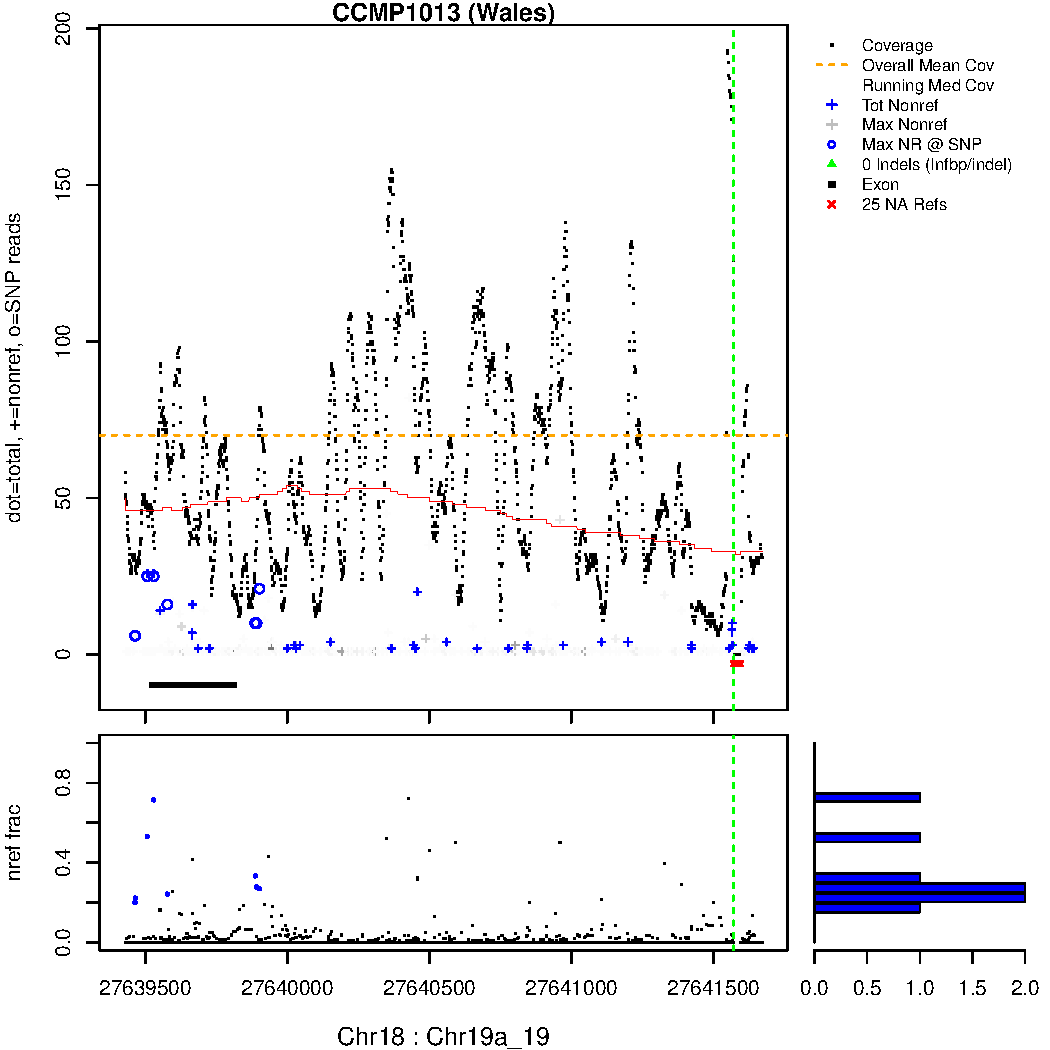
\includegraphics[width=\maxwidth]{figs-knitr/unnamed-chunk-17-1} 
\begin{kframe}\begin{alltt}
\hlstd{des.df[[}\hlnum{3}\hlstd{]][}\hlnum{10}\hlstd{,]}
\end{alltt}
\begin{verbatim}
#     Chr  Start    End Length iStart   iEnd
# 10 Chr1 222626 224906   2281 222626 224906
\end{verbatim}
\begin{alltt}
\hlkwd{seedesert}\hlstd{(}\hlnum{3}\hlstd{,}\hlnum{10}\hlstd{,} \hlnum{300}\hlstd{)}   \hlcom{# desert +/-300 bp}
\end{alltt}
\end{kframe}
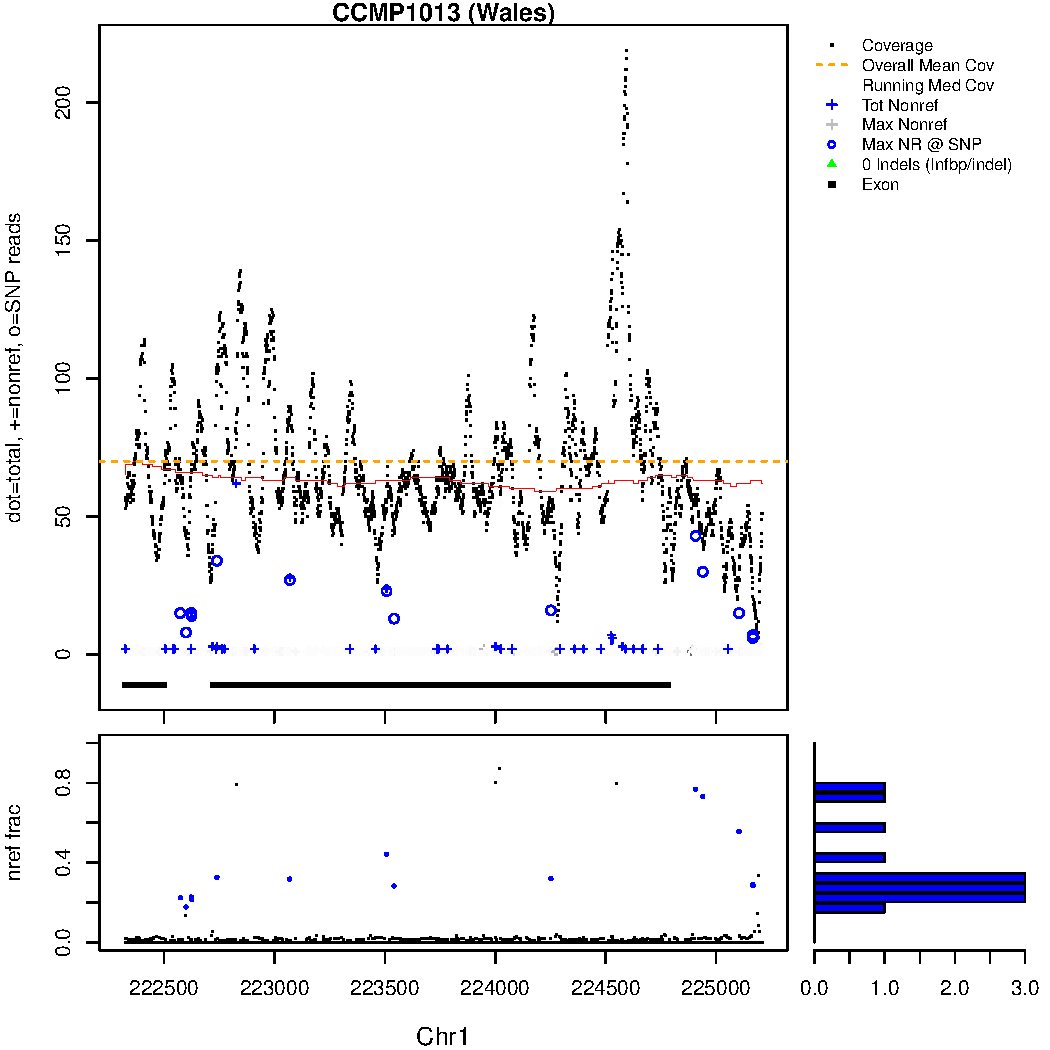
\includegraphics[width=\maxwidth]{figs-knitr/unnamed-chunk-17-2} 
\begin{kframe}\begin{alltt}
\hlkwd{seecounts}\hlstd{(}\hlnum{222626}\hlopt{+}\hlkwd{c}\hlstd{(}\hlopt{-}\hlnum{2}\hlstd{,}\hlopt{-}\hlnum{1}\hlstd{,}\hlnum{0}\hlstd{),}\hlnum{3}\hlstd{,snp.tables.full)}
\end{alltt}
\begin{verbatim}
#    chr    pos Ref Strain  A  G  C  T SNP  exon indel nrf rat
# 1 Chr1 222624   A                                           
# 2                   1013 51 15  0  0   1 FALSE FALSE        
# 3 Chr1 222625   T                                           
# 4                   1013  1  0 14 51   1 FALSE FALSE        
# 5 Chr1 222626   A                                           
# 6                   1013 66  1  0  0   0 FALSE FALSE
\end{verbatim}
\begin{alltt}
\hlkwd{seecounts}\hlstd{(}\hlnum{224906}\hlopt{+}\hlstd{(}\hlopt{-}\hlnum{2}\hlopt{:}\hlnum{2}\hlstd{),}\hlnum{3}\hlstd{,snp.tables.full)}
\end{alltt}
\begin{verbatim}
#     chr    pos Ref Strain  A  G C  T SNP  exon indel nrf rat
# 1  Chr1 224904   G                                          
# 2                    1013  0 56 0  0   0 FALSE FALSE        
# 3  Chr1 224905   A                                          
# 4                    1013 58  0 0  0   0 FALSE FALSE        
# 5  Chr1 224906   G                                          
# 6                    1013  0 58 0  0   0 FALSE FALSE        
# 7  Chr1 224907   A                                          
# 8                    1013 13 43 0  0   1 FALSE FALSE        
# 9  Chr1 224908   T                                          
# 10                   1013  0  0 0 57   0 FALSE FALSE
\end{verbatim}
\begin{alltt}
\hlstd{snp.tables.full[[}\hlnum{3}\hlstd{]]}\hlopt{$}\hlstd{snp[}\hlnum{224901}\hlopt{:}\hlnum{225200}\hlstd{]}
\end{alltt}
\begin{verbatim}
#   [1] 0 0 0 0 0 0 1 0 0 0 0 0 0 0 0 0 0 0 0 0 0 0 0 0 0 0 0 0 0 0 0 0 0 0 0 0 0 0 0 1 0 0 0 0 0 0
#  [47] 0 0 0 0 0 0 0 0 0 0 0 0 0 0 0 0 0 0 0 0 0 0 0 0 0 0 0 0 0 0 0 0 0 0 0 0 0 0 0 0 0 0 0 0 0 0
#  [93] 0 0 0 0 0 0 0 0 0 0 0 0 0 0 0 0 0 0 0 0 0 0 0 0 0 0 0 0 0 0 0 0 0 0 0 0 0 0 0 0 0 0 0 0 0 0
# [139] 0 0 0 0 0 0 0 0 0 0 0 0 0 0 0 0 0 0 0 0 0 0 0 0 0 0 0 0 0 0 0 0 0 0 0 0 0 0 0 0 0 0 0 0 0 0
# [185] 0 0 0 0 0 0 0 0 0 0 0 0 0 0 0 0 0 0 0 1 0 0 0 0 0 0 0 0 0 0 0 0 0 0 0 0 0 0 0 0 0 0 0 0 0 0
# [231] 0 0 0 0 0 0 0 0 0 0 0 0 0 0 0 0 0 0 0 0 0 0 0 0 0 0 0 0 0 0 0 0 0 0 0 1 1 0 0 0 0 0 0 0 0 0
# [277] 0 0 0 0 0 0 0 0 0 0 0 0 0 0 0 0 0 0 0 0 0 0 0 0
\end{verbatim}
\end{kframe}
\end{knitrout}

Desert at row 10 starts immediately after the adjacent pair of snps at 222624:222625 (in the cluster of snps in the non-exonic region at left in the plot), and extends up to but not including 224907, the 6th SNP following the start (the first in the cluster of 5 following the exon).  That cluster of 5 spans less than 300 bp, so position 222906, e.g., is definitely NOT sufficiently far from 5th snp to be $10^{-4}$ in neg bin model.  \emph{So}, I presume we have \emph{not} yet correctly described how deserts are defined... Aha, START at a position $<10^{-4}$, then include up to but not including 5th snp.  

\section{Deserts-by-Chance}
\label{sec:sim}

What would we expect by chance?  Simple theoretical model: let $x_i$ be an indicator variable, 1 if genome pos $i$ has its 5th SNP so far away that prob is $<10^{-4}$, else 0.  Expected number of such positions is genome len times $10^{-4}\approx3200$.  Ignoring merging (which I expect to be rare with random snp placement), the first of every run of such positions starts a desert, and since P(desert length == $x$) declines rapidly with $x$, I would expect most such runs to be short, say ballpark 100 when des.threshold is 2-3K, so the NUMBER of deserts should be small (ballpark 3200/100=32?), and their total LENGTH should be ballpark 3200 plus des.threshold per desert, which should be less than about 100Kb (3.2Kb + 32 x 3000).

\subsection{Simple Simulation}
It's probably tractable to calculate the parameters above analytically, but the following simple simulation roughly replicates this.  Drop SNPs at random at rate $p$ (approx NY rate) on genome of length $n=32$ Mb, using corresponding des.threshold $L$.  Find all ``gap lengths'' (= distance from start of genome/a snp to (but excluding) 5th subsequent snp). Any snp where $gaps > L$ starts a desert; length of that gap minus $L$ approximates ``sum of $x_i$'' above, and sum of all gaps longer than $L$ approximates total desert length.  Repeat 20 times and output summary stats. 

\begin{knitrout}\footnotesize
\definecolor{shadecolor}{rgb}{0.969, 0.969, 0.969}\color{fgcolor}\begin{kframe}
\begin{alltt}
\hlstd{des.sim} \hlkwb{<-} \hlkwa{function}\hlstd{(}\hlkwc{p}\hlstd{=}\hlnum{1}\hlopt{/}\hlnum{200}\hlstd{,}
                    \hlkwc{n}\hlstd{=}\hlkwd{genome.length.constants}\hlstd{()}\hlopt{$}\hlstd{genome.length.trunc,}
                    \hlkwc{L}\hlstd{=}\hlkwd{qnbinom}\hlstd{(}\hlnum{1e-4}\hlstd{,}\hlnum{5}\hlstd{,p,}\hlkwc{lower.tail}\hlstd{=F))\{}
  \hlstd{out.df} \hlkwb{<-} \hlkwa{NULL}
  \hlkwa{for}\hlstd{(i} \hlkwa{in} \hlnum{1}\hlopt{:}\hlnum{20}\hlstd{)\{}
    \hlstd{faux.snps}   \hlkwb{<-} \hlkwd{sample}\hlstd{(n,p}\hlopt{*}\hlstd{n)}
    \hlstd{sorted.faux} \hlkwb{<-} \hlkwd{sort}\hlstd{(faux.snps)}
    \hlstd{n.faux} \hlkwb{<-} \hlkwd{length}\hlstd{(sorted.faux)}
    \hlstd{gaps}   \hlkwb{<-} \hlkwd{c}\hlstd{(sorted.faux[}\hlnum{5}\hlopt{:}\hlstd{n.faux],n}\hlopt{+}\hlnum{1}\hlstd{)}\hlopt{-}\hlkwd{c}\hlstd{(}\hlnum{0}\hlstd{,sorted.faux[}\hlnum{1}\hlopt{:}\hlstd{(n.faux}\hlopt{-}\hlnum{4}\hlstd{)])}\hlopt{-}\hlnum{1}
    \hlstd{out.df} \hlkwb{<-} \hlkwd{rbind}\hlstd{(out.df,} \hlkwd{data.frame}\hlstd{(}\hlkwc{number.of.deserts}\hlstd{=}\hlkwd{sum}\hlstd{(gaps} \hlopt{>} \hlstd{L),}
                                       \hlkwc{des.len.minus.L}  \hlstd{=}\hlkwd{sum}\hlstd{(}\hlkwd{pmax}\hlstd{(}\hlnum{0}\hlstd{, gaps} \hlopt{-} \hlstd{L)),}
                                       \hlkwc{des.len}          \hlstd{=}\hlkwd{sum}\hlstd{(gaps[gaps} \hlopt{>} \hlstd{L]),}
                                       \hlkwc{max.len}          \hlstd{=}\hlkwd{max}\hlstd{(gaps)))}
  \hlstd{\}}
  \hlstd{out.df} \hlkwb{<-} \hlkwd{rbind}\hlstd{(out.df,} \hlkwc{mu}\hlstd{=}\hlkwd{data.frame}\hlstd{(}\hlkwc{number.of.deserts}\hlstd{=}\hlkwd{round}\hlstd{(}\hlkwd{mean}\hlstd{(out.df[,}\hlnum{1}\hlstd{])),}
                                        \hlkwc{des.len.minus.L}  \hlstd{=}\hlkwd{round}\hlstd{(}\hlkwd{mean}\hlstd{(out.df[,}\hlnum{2}\hlstd{])),}
                                        \hlkwc{des.len}          \hlstd{=}\hlkwd{round}\hlstd{(}\hlkwd{mean}\hlstd{(out.df[,}\hlnum{3}\hlstd{])),}
                                        \hlkwc{max.len}          \hlstd{=}\hlkwd{round}\hlstd{(}\hlkwd{mean}\hlstd{(out.df[,}\hlnum{4}\hlstd{]))))}
  \hlkwd{return}\hlstd{(out.df)}
\hlstd{\}}

\hlkwd{des.sim}\hlstd{()}
\end{alltt}
\begin{verbatim}
#    number.of.deserts des.len.minus.L des.len max.len
# 1                 16            3348   60068    4210
# 2                 26            6506   98676    4186
# 3                 14            3977   53607    4557
# 4                  4             982   15162    4167
# 5                 26           10734  102904    4571
# 6                 14            3721   53351    4246
# 7                 13            3097   49182    4159
# 8                 31            7182  117077    4345
# 9                 14            4174   53804    4570
# 10                23            5464   86999    4413
# 11                23            6011   87546    4660
# 12                21            5805   80250    4558
# 13                17            3036   63301    4188
# 14                19            7000   74355    4885
# 15                18            4177   67987    4007
# 16                21            4158   78603    4154
# 17                10            1158   36608    3840
# 18                 9            1546   33451    4020
# 19                14            2931   52561    4039
# 20                31            8436  118331    4156
# mu                18            4672   69191    4297
\end{verbatim}
\end{kframe}
\end{knitrout}

Averages are in line with ``ballpark numbers'' above: $<$20 deserts, $<$4Kb total of ``excess desert'' (length in excess of $L$), and $<$100Kb total desert. 

Repeat with Wales param; similar results:

\begin{knitrout}\footnotesize
\definecolor{shadecolor}{rgb}{0.969, 0.969, 0.969}\color{fgcolor}\begin{kframe}
\begin{alltt}
\hlkwd{des.sim}\hlstd{(}\hlkwc{p}\hlstd{=}\hlnum{1}\hlopt{/}\hlnum{122.9541}\hlstd{)}
\end{alltt}
\begin{verbatim}
#    number.of.deserts des.len.minus.L des.len max.len
# 1                 19            3715   45040    2819
# 2                 16            2722   37522    2559
# 3                 30            4491   69741    2688
# 4                 17            1180   38155    2466
# 5                 15            1890   34515    2727
# 6                 24            4078   56278    2912
# 7                 17            1704   38679    2432
# 8                 33            4975   76750    2706
# 9                 18            2073   41223    2610
# 10                26            3113   59663    2501
# 11                20            2913   46413    2716
# 12                54           10206  127656    2864
# 13                35            6689   82814    2940
# 14                18            3758   42908    2768
# 15                39            5624   90449    2698
# 16                27            3462   62187    2672
# 17                19            1550   42875    2432
# 18                26            3937   60487    2631
# 19                26            2750   59300    2651
# 20                27            4984   63709    2680
# mu                25            3791   58818    2674
\end{verbatim}
\end{kframe}
\end{knitrout}

In short, all way lower than observed in Thaps. \emph{I suspect} that this difference is partially due to the fact that our global snp rate estimates lump together coding and noncoding; even though they differ by only about 1.5x, the cummulative effect of the lower exonic rate over a long exon frequently reaches our statistical significance threshold.  Modeling that would probably generate a number of small deserts.  

\subsection{One-Giant-Exon Simulation}
\label{sec:giant-exon}
To test the above suggestion, look at simulation like above, but using the same (genome-wide) $L$ threshold with the lower exonic SNP rate, on a ``genome'' of length equal to the total exonic content.

\begin{knitrout}\footnotesize
\definecolor{shadecolor}{rgb}{0.969, 0.969, 0.969}\color{fgcolor}\begin{kframe}
\begin{alltt}
\hlkwd{nrow}\hlstd{(snp.tables.full[[}\hlnum{1}\hlstd{]])}                     \hlcom{# these tables have full genome}
\end{alltt}
\begin{verbatim}
# [1] 32610006
\end{verbatim}
\begin{alltt}
\hlkwd{genome.length.constants}\hlstd{()}\hlopt{$}\hlstd{genome.length.full}
\end{alltt}
\begin{verbatim}
# [1] 32610006
\end{verbatim}
\begin{alltt}
\hlkwd{genome.length.constants}\hlstd{()}\hlopt{$}\hlstd{genome.length.trunc}  \hlcom{# but I only want Chr's (no organelles, BD_)}
\end{alltt}
\begin{verbatim}
# [1] 31301782
\end{verbatim}
\begin{alltt}
\hlstd{exonic} \hlkwb{<-} \hlkwd{sum}\hlstd{(snp.tables.full[[}\hlnum{1}\hlstd{]]}\hlopt{$}\hlstd{exon[}\hlnum{1}\hlopt{:}\hlkwd{genome.length.constants}\hlstd{()}\hlopt{$}\hlstd{genome.length.trunc])}
\hlstd{exonic}
\end{alltt}
\begin{verbatim}
# [1] 18862325
\end{verbatim}
\end{kframe}
\end{knitrout}
\begin{knitrout}\footnotesize
\definecolor{shadecolor}{rgb}{0.969, 0.969, 0.969}\color{fgcolor}\begin{kframe}
\begin{alltt}
\hlstd{des.sim2} \hlkwb{<-} \hlkwa{function}\hlstd{(}\hlkwc{p} \hlstd{=} \hlnum{1}\hlopt{/}\hlnum{200}\hlstd{,} \hlkwc{n} \hlstd{=} \hlkwd{genome.length.constants}\hlstd{()}\hlopt{$}\hlstd{genome.length.trunc)\{}
  \hlstd{L} \hlkwb{<-} \hlkwd{qnbinom}\hlstd{(}\hlnum{1e-4}\hlstd{,}\hlnum{5}\hlstd{,p,}\hlkwc{lower.tail}\hlstd{=F)}
  \hlstd{p2} \hlkwb{<-} \hlstd{p}\hlopt{/}\hlnum{1.5}                                  \hlcom{# p2 is approx exonic SNP rate}
  \hlkwd{cat}\hlstd{(}\hlstr{'Ditto, but ~exonic p2 ='}\hlstd{, p2,} \hlstr{'exonic ='}\hlstd{, exonic,} \hlstr{'L ='}\hlstd{, L,} \hlstr{':\textbackslash{}n'}\hlstd{)}
  \hlstd{out2.df} \hlkwb{<-} \hlkwd{des.sim}\hlstd{(p2,exonic,L)}
  \hlkwd{print}\hlstd{(out2.df)}
\hlstd{\}}
\end{alltt}
\end{kframe}
\end{knitrout}
\begin{knitrout}\footnotesize
\definecolor{shadecolor}{rgb}{0.969, 0.969, 0.969}\color{fgcolor}\begin{kframe}
\begin{alltt}
\hlkwd{des.sim2}\hlstd{(}\hlkwc{p}\hlstd{=}\hlnum{1}\hlopt{/}\hlnum{200}\hlstd{)}       \hlcom{# ~ NY SNP rate}
\end{alltt}
\begin{verbatim}
# Ditto, but ~exonic p2 = 0.003333333 exonic = 18862325 L = 3545 :
#    number.of.deserts des.len.minus.L des.len max.len
# 1                522          189327 2039817    5317
# 2                511          233580 2045075    6192
# 3                512          195260 2010300    5532
# 4                569          244005 2261110    6791
# 5                563          250553 2246388    7419
# 6                517          185020 2017785    5275
# 7                526          206692 2071362    5870
# 8                500          207244 1979744    6504
# 9                523          244271 2098306    6072
# 10               616          268617 2452337    5706
# 11               497          194843 1956708    5709
# 12               558          204602 2182712    5323
# 13               633          268031 2512016    5716
# 14               548          235667 2178327    5882
# 15               498          203535 1968945    5842
# 16               562          250833 2243123    5988
# 17               564          238438 2237818    6866
# 18               517          208806 2041571    5611
# 19               552          225441 2182281    5784
# 20               490          189028 1926078    5673
# mu               539          222190 2132590    5954
\end{verbatim}
\begin{alltt}
\hlkwd{des.sim2}\hlstd{(}\hlkwc{p}\hlstd{=}\hlnum{1}\hlopt{/}\hlnum{122.9541}\hlstd{)}  \hlcom{# ~ Wales SNP rate}
\end{alltt}
\begin{verbatim}
# Ditto, but ~exonic p2 = 0.005422078 exonic = 18862325 L = 2175 :
#    number.of.deserts des.len.minus.L des.len max.len
# 1                848          191305 2035705    3627
# 2                913          232634 2218409    3614
# 3                828          204315 2005215    4129
# 4                791          211439 1931864    3742
# 5                896          236854 2185654    3716
# 6                840          217236 2044236    3634
# 7                886          238365 2165415    4251
# 8                778          186605 1878755    3632
# 9                850          214977 2063727    4645
# 10               831          210242 2017667    3984
# 11               816          210534 1985334    3648
# 12               995          270335 2434460    3858
# 13               731          177523 1767448    3372
# 14               978          250682 2377832    3457
# 15               791          207807 1928232    4482
# 16               900          227793 2185293    3501
# 17               799          208771 1946596    3660
# 18               873          213779 2112554    3792
# 19               919          231637 2230462    3916
# 20               890          215402 2151152    3978
# mu               858          217912 2083300    3832
\end{verbatim}
\end{kframe}
\end{knitrout}

This is a significant overestimate of ``false positives'' since the real genome is a mix of exon/non-exon and few exons have length $>L$.  Furthermore, stats given elsewhere showed that deserts are not sharply enriched for exonic content, but overall it does suggest that \textit{small} desert predictions include many false positives from our simple model, but our \textit{big} deserts are extremely unlikely to be false positives; the largest deserts seen in these simulations ($\approx7$Kb) are only about twice as long as the min desert.  But of course the model could be made more realistic.

\subsection{A Permutation Test}
Here's an alternate tack:  permute SNP positions in exons seperately from permuted SNP positions in non-exons, then look at gaps/desert predictions.

\begin{knitrout}\footnotesize
\definecolor{shadecolor}{rgb}{0.969, 0.969, 0.969}\color{fgcolor}\begin{kframe}
\begin{alltt}
\hlstd{des.perm} \hlkwb{<-} \hlkwa{function}\hlstd{(} \hlkwc{st}\hlstd{=}\hlnum{7}\hlstd{,} \hlkwc{p}\hlstd{=}\hlkwa{NULL}\hlstd{,} \hlkwc{times}\hlstd{=}\hlnum{20}\hlstd{)\{}
  \hlstd{nn} \hlkwb{<-} \hlkwd{genome.length.constants}\hlstd{()}\hlopt{$}\hlstd{genome.length.trunc}
  \hlstd{sim.ex}  \hlkwb{<-} \hlstd{snp.tables.full[[st]]}\hlopt{$}\hlstd{exon[}\hlnum{1}\hlopt{:}\hlstd{nn]}
  \hlstd{sim.snp} \hlkwb{<-} \hlstd{snp.tables.full[[st]]}\hlopt{$}\hlstd{snp [}\hlnum{1}\hlopt{:}\hlstd{nn]}
  \hlkwa{if}\hlstd{(}\hlkwd{is.null}\hlstd{(p))\{}
    \hlstd{p} \hlkwb{<-} \hlkwd{sum}\hlstd{(sim.snp)}\hlopt{/}\hlstd{nn}
  \hlstd{\}}
  \hlstd{L} \hlkwb{<-} \hlkwd{qnbinom}\hlstd{(}\hlnum{1e-4}\hlstd{,}\hlnum{5}\hlstd{,p,}\hlkwc{lower.tail}\hlstd{=F)}
  \hlstd{sim.nex} \hlkwb{<-} \hlkwd{sum}\hlstd{(sim.ex)}
  \hlkwd{cat}\hlstd{(}\hlstr{'Permuted Desert Test: strain'}\hlstd{, st,} \hlstr{', p ='}\hlstd{, p,} \hlstr{', L ='}\hlstd{, L,} \hlstr{'\textbackslash{}n'}\hlstd{)}
  \hlstd{out.df} \hlkwb{<-} \hlkwa{NULL}
  \hlstd{gapl} \hlkwb{<-} \hlkwa{NULL}
  \hlkwa{for} \hlstd{(i} \hlkwa{in} \hlnum{1}\hlopt{:}\hlstd{times)\{}
    \hlstd{sim.snp[ sim.ex]} \hlkwb{<-} \hlkwd{sample}\hlstd{(sim.snp[ sim.ex],    sim.nex,} \hlkwc{replace}\hlstd{=}\hlnum{FALSE}\hlstd{)}
    \hlstd{sim.snp[}\hlopt{!}\hlstd{sim.ex]} \hlkwb{<-} \hlkwd{sample}\hlstd{(sim.snp[}\hlopt{!}\hlstd{sim.ex], nn}\hlopt{-}\hlstd{sim.nex,} \hlkwc{replace}\hlstd{=}\hlnum{FALSE}\hlstd{)}
    \hlstd{sorted.faux} \hlkwb{<-} \hlkwd{which}\hlstd{(sim.snp}\hlopt{==}\hlnum{1}\hlstd{)}

    \hlstd{n.faux} \hlkwb{<-} \hlkwd{length}\hlstd{(sorted.faux)}
    \hlstd{gaps}   \hlkwb{<-} \hlkwd{c}\hlstd{(sorted.faux[}\hlnum{5}\hlopt{:}\hlstd{n.faux],n}\hlopt{+}\hlnum{1}\hlstd{)}\hlopt{-}\hlkwd{c}\hlstd{(}\hlnum{0}\hlstd{,sorted.faux[}\hlnum{1}\hlopt{:}\hlstd{(n.faux}\hlopt{-}\hlnum{4}\hlstd{)])}\hlopt{-}\hlnum{1}
    \hlstd{out.df} \hlkwb{<-} \hlkwd{rbind}\hlstd{(out.df,} \hlkwd{data.frame}\hlstd{(}\hlkwc{number.of.deserts}\hlstd{=}\hlkwd{sum}\hlstd{(gaps} \hlopt{>} \hlstd{L),}
                                       \hlkwc{des.len.minus.L}  \hlstd{=}\hlkwd{sum}\hlstd{(}\hlkwd{pmax}\hlstd{(}\hlnum{0}\hlstd{, gaps} \hlopt{-} \hlstd{L)),}
                                       \hlkwc{des.len}          \hlstd{=}\hlkwd{sum}\hlstd{(gaps[gaps} \hlopt{>} \hlstd{L]),}
                                       \hlkwc{max.len}          \hlstd{=}\hlkwd{max}\hlstd{(gaps)))}
    \hlstd{gapl} \hlkwb{<-} \hlkwd{c}\hlstd{(gapl, gaps[gaps} \hlopt{>} \hlstd{L])}
  \hlstd{\}}
  \hlstd{out.df} \hlkwb{<-} \hlkwd{rbind}\hlstd{(out.df,} \hlkwc{mu}\hlstd{=}\hlkwd{data.frame}\hlstd{(}\hlkwc{number.of.deserts}\hlstd{=}\hlkwd{round}\hlstd{(}\hlkwd{mean}\hlstd{(out.df[,}\hlnum{1}\hlstd{])),}
                                        \hlkwc{des.len.minus.L}  \hlstd{=}\hlkwd{round}\hlstd{(}\hlkwd{mean}\hlstd{(out.df[,}\hlnum{2}\hlstd{])),}
                                        \hlkwc{des.len}          \hlstd{=}\hlkwd{round}\hlstd{(}\hlkwd{mean}\hlstd{(out.df[,}\hlnum{3}\hlstd{])),}
                                        \hlkwc{max.len}          \hlstd{=}\hlkwd{round}\hlstd{(}\hlkwd{mean}\hlstd{(out.df[,}\hlnum{4}\hlstd{]))))}
  \hlkwd{cat}\hlstd{(}\hlstr{'Number of deserts in'}\hlstd{, times,} \hlstr{'trials:'}\hlstd{,} \hlkwd{length}\hlstd{(gapl),} \hlstr{', length distribution:\textbackslash{}n'}\hlstd{)}
  \hlkwd{print}\hlstd{(}\hlkwd{c}\hlstd{(}\hlkwd{summary}\hlstd{(gapl),}\hlkwc{SD}\hlstd{=}\hlkwd{sd}\hlstd{(gapl)))}
  \hlkwd{return}\hlstd{(}\hlkwd{list}\hlstd{(}\hlkwc{des.lengths}\hlstd{=gapl,} \hlkwc{twenty}\hlstd{=out.df))}
\hlstd{\}}
\end{alltt}
\end{kframe}
\end{knitrout}
\begin{knitrout}\footnotesize
\definecolor{shadecolor}{rgb}{0.969, 0.969, 0.969}\color{fgcolor}\begin{kframe}
\begin{alltt}
\hlstd{dp7} \hlkwb{<-} \hlkwd{des.perm}\hlstd{(}\hlnum{7}\hlstd{)}
\end{alltt}
\begin{verbatim}
# Permuted Desert Test: strain 7 , p = 0.004916685 , L = 3605 
# Number of deserts in 20 trials: 439 , length distribution:
#      Min.   1st Qu.    Median      Mean   3rd Qu.      Max.        SD 
# 3606.0000 3673.0000 3785.0000 3879.2551 3987.5000 5617.0000  285.5675
\end{verbatim}
\begin{alltt}
\hlstd{dp7}\hlopt{$}\hlstd{twenty}
\end{alltt}
\begin{verbatim}
#    number.of.deserts des.len.minus.L des.len max.len
# 1                 22            4401   83711    4144
# 2                 17            3336   64621    4133
# 3                  8            3777   32617    4681
# 4                 27            5590  102925    4389
# 5                 35           11671  137846    4864
# 6                 27           10408  107743    4509
# 7                 18            3445   68335    4245
# 8                 16            4541   62221    4647
# 9                 18            3982   68872    4207
# 10                26            7491  101221    4674
# 11                18            5007   69897    4495
# 12                23            5284   88199    4611
# 13                23            7315   90230    4749
# 14                19            4892   73387    4534
# 15                38           11456  148446    5043
# 16                18            3679   68569    4475
# 17                25           10937  101062    5617
# 18                10            1273   37323    3903
# 19                27            5987  103322    4312
# 20                24            5926   92446    4624
# mu                22            6020   85150    4543
\end{verbatim}
\end{kframe}
\end{knitrout}
\begin{knitrout}\footnotesize
\definecolor{shadecolor}{rgb}{0.969, 0.969, 0.969}\color{fgcolor}\begin{kframe}
\begin{alltt}
\hlstd{dp3} \hlkwb{<-} \hlkwd{des.perm}\hlstd{(}\hlnum{3}\hlstd{)}
\end{alltt}
\begin{verbatim}
# Permuted Desert Test: strain 3 , p = 0.00791447 , L = 2235 
# Number of deserts in 20 trials: 1046 , length distribution:
#      Min.   1st Qu.    Median      Mean   3rd Qu.      Max.        SD 
# 2236.0000 2289.0000 2357.0000 2410.7438 2475.5000 3262.0000  169.0779
\end{verbatim}
\begin{alltt}
\hlstd{dp3}\hlopt{$}\hlstd{twenty}
\end{alltt}
\begin{verbatim}
#    number.of.deserts des.len.minus.L des.len max.len
# 1                 54           10390  131080    3115
# 2                 41            6213   97848    2865
# 3                 43            5591  101696    2705
# 4                 57           11815  139210    2921
# 5                 33            6056   79811    3230
# 6                 61            9311  145646    2764
# 7                 42            7294  101164    2799
# 8                 57           10356  137751    2923
# 9                 55           10679  133604    3204
# 10                62            9482  148052    3245
# 11                64           11655  154695    3192
# 12                50            8855  120605    2735
# 13                63           13445  154250    3254
# 14                46            6527  109337    2694
# 15                63           10149  150954    2843
# 16                66           11906  159416    2869
# 17                49           11499  121014    3262
# 18                39            5656   92821    2824
# 19                48            7590  114870    2790
# 20                53            9359  127814    3247
# mu                52            9191  126082    2974
\end{verbatim}
\begin{alltt}
\hlstd{opar} \hlkwb{<-} \hlkwd{par}\hlstd{(}\hlkwc{mfrow}\hlstd{=}\hlkwd{c}\hlstd{(}\hlnum{1}\hlstd{,}\hlnum{2}\hlstd{),} \hlkwc{no.readonly}\hlstd{=}\hlnum{TRUE}\hlstd{)}
\hlkwd{hist}\hlstd{(dp7}\hlopt{$}\hlstd{des.lengths)}
\hlkwd{hist}\hlstd{(dp3}\hlopt{$}\hlstd{des.lengths)}
\end{alltt}
\end{kframe}
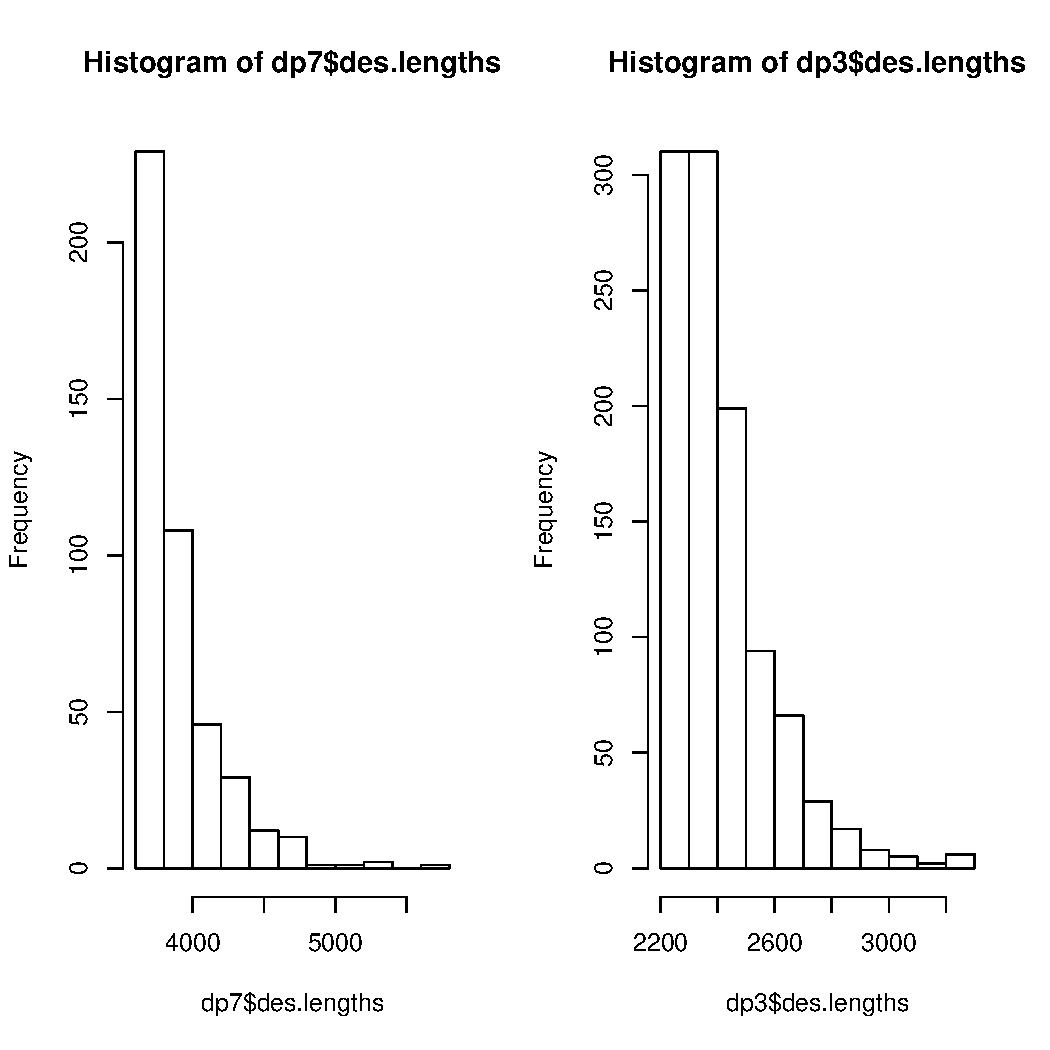
\includegraphics[width=\maxwidth]{figs-knitr/unnamed-chunk-25-1} 
\begin{kframe}\begin{alltt}
\hlkwd{par}\hlstd{(opar)}
\end{alltt}
\end{kframe}
\end{knitrout}

So, treating exons/non-exons separately does increase the number and size of deserts a bit, but not nearly as drastically as the giant exon model in \ref{sec:giant-exon}.  This permutation test is probably a bit anti-conservative, since lumping SNP rates into just two classes underestimates the heterogeneity of the genome.  However, based on all of the simulation results, even one desert of 50Kb or longer (let alone the $\approx29$ seen in L-clade) is very improbable---50Kb is roughly 10x longer than the longest desert seen in any of our random trials and more than 100$\sigma$ above the mean seen in the permutations tests.

\textbf{Bottom Line:}
The big deserts are so large and so strongly depleted of SNPs that they will not arise from our simple null model, even after accounting for differential SNP rates in exons.  Deserts on the scale of genes, however, are likely to reflect purifying selection in at least some cases.

% remember to do this to enable Id keyword substution: svn propset svn:keywords Id nc-snps.rnw 
\vfill\footnotesize\flushright SVN ID I miss you. $ $Id: nc-snps 2017-07-19 or later.$ $
\end{document}
